\documentclass[a4paper]{article}
\usepackage{a4wide,amssymb,epsfig,latexsym,multicol,array,hhline,fancyhdr,amsthm}
\usepackage{vntex}
\usepackage{amsmath}
\usepackage{lastpage}
\usepackage{longtable}
\usepackage{booktabs}
\usepackage{tabularx, caption}
\usepackage{multirow}
\usepackage{multicol}
\usepackage[lined,boxed,commentsnumbered]{algorithm2e}
\usepackage{enumerate}
\usepackage{color}
\usepackage{graphicx}							% Standard graphics package
\usepackage{array}
\usepackage{tabularx, caption}
\usepackage{multirow}
\usepackage{listings}
\usepackage{color} % tô màu cho code
\usepackage{multicol}
\usepackage{rotating}
\usepackage{graphics}
\usepackage{float}
\usepackage{geometry}
\usepackage{setspace}
\usepackage{indentfirst} 
\usepackage{epsfig}
\usepackage{tikz}
\usetikzlibrary{arrows,snakes,backgrounds}
\usepackage{hyperref}
\hypersetup{urlcolor=blue,linkcolor=black,citecolor=black,colorlinks=true} 
\usepackage[most]{tcolorbox}
\newtcolorbox{tcbdoublebox}[1][]{
  enhanced jigsaw,
  sharp corners,
  colback=white,
  colframe=teal,
  borderline={1pt}{-2pt}{teal},
  fontupper={\setlength{\parindent}{20pt}},
  #1
}
%\usepackage{pstcol} 								% PSTricks with the standard color package
\newtheorem*{solution}{Cách giải}
\newtheorem{example}{Ví dụ}
\newtheorem{step}{Bước}
\newtheorem*{nhanxet}{Nhận xét}
\newtheorem{case}{Trường hợp}
\newtheorem{definition}{Định nghĩa}
\newtheorem{theorem}{{\bf Theorem}}
\newtheorem{property}{{\bf Property}}
\newtheorem{proposition}{{\bf Proposition}}
\newtheorem{corollary}[proposition]{{\bf Corollary}}
\newtheorem{lemma}[proposition]{{\bf Lemma}}
\newtheorem*{problem}{Problem}
\newtheorem*{sol}{Solution}
\AtBeginDocument{\renewcommand*\contentsname{Contents}}
\AtBeginDocument{\renewcommand*\refname{References}}
%\usepackage{fancyhdr}
\setlength{\headheight}{40pt}
\pagestyle{fancy}
\fancyhead{} % clear all header fields
\fancyhead[L]{
 \begin{tabular}{rl}
    \begin{picture}(25,15)(0,0)
    \put(0,-8){
\includegraphics[width=8mm, height=8mm]{hcmut.png}}
    %\put(0,-8){\epsfig{width=10mm,figure=hcmut.eps}}
   \end{picture}&
	%
\includegraphics[width=8mm, height=8mm]{hcmut.png} & %
	\begin{tabular}{l}
		\textbf{\bf \ttfamily University of Technology, Ho Chi Minh City}\\
		\textbf{\bf \ttfamily Faculty of Computer Science and Engineering}
	\end{tabular} 	
 \end{tabular}
}
\fancyhead[R]{
	\begin{tabular}{l}
		\tiny \bf \\
		\tiny \bf 
	\end{tabular}  }
\fancyfoot{} % clear all footer fields
\fancyfoot[L]{\scriptsize \ttfamily Assignment for Mathematical Modeling - Academic year 2021 - 2022}
\fancyfoot[R]{\scriptsize \ttfamily Page {\thepage}/\pageref{LastPage}}
\renewcommand{\headrulewidth}{0.3pt}
\renewcommand{\footrulewidth}{0.3pt}


%%%
\setcounter{secnumdepth}{4}
\setcounter{tocdepth}{3}
\makeatletter
\newcounter {subsubsubsection}[subsubsection]
\renewcommand\thesubsubsubsection{\thesubsubsection .\@alph\c@subsubsubsection}
\newcommand\subsubsubsection{\@startsection{subsubsubsection}{4}{\z@}%
                                     {-3.25ex\@plus -1ex \@minus -.2ex}%
                                     {1.5ex \@plus .2ex}%
                                     {\normalfont\normalsize\bfseries}}
\newcommand*\l@subsubsubsection{\@dottedtocline{3}{10.0em}{4.1em}}
\newcommand*{\subsubsubsectionmark}[1]{}
\makeatother

\usepackage{indentfirst}
\setlength{\parindent}{0pt}
\definecolor{dkgreen}{rgb}{0,0.6,0}
\definecolor{gray}{rgb}{0.5,0.5,0.5}
\definecolor{mauve}{rgb}{0.58,0,0.82}
\lstset{frame=tb,
  language=Python,
 numbers=left, numberstyle=\tiny,
  stepnumber = 5, numbersep=5pt, keywordstyle=\color{blue}
  }


\begin{document}

\begin{titlepage}
\begin{center}
VIETNAM NATIONAL UNIVERSITY, HO CHI MINH CITY \\
UNIVERSITY OF TECHNOLOGY \\
FACULTY OF COMPUTER SCIENCE AND ENGINEERING
\end{center}

\vspace{1cm}

\begin{figure}[h!]
\begin{center}

\includegraphics[width=3cm]{hcmut.png}
\end{center}
\end{figure}

\vspace{1cm}


\begin{center}
\begin{tabular}{c}
\multicolumn{1}{l}{\textbf{{\Large MÔ HÌNH HÓA TOÁN HỌC (CO2011)}}}\\
~~\\
\hline
\\
\multicolumn{1}{l}{\textbf{{\Large Assignment}}}\\
\\
\\
\textbf{\textit{{\Huge "Dynamics of Love"}}}\\
\\
\\
\hline
\end{tabular}
\end{center}

\vspace{2cm}

\begin{table}[h]
\begin{tabular}{rrlrr}
\hspace{3 cm} & \textbf{Advisors}: & Mai Xuân Toàn&\\
& & Trần Hồng Tài&\\
& & Nguyễn An Khương& \\
& & Nguyễn Tiến Thịnh& \\
& & Nguyễn Văn Minh Mẫn& \\
& & & & \\
& \textbf{Students}: & Nguyễn Tuấn Minh  - 2110359 \textit{(Group L05 - Team 38, Leader)} \\
& & Trần Nguyễn Thái Bình - 2110051 \textit{(Group L05 - Team 38)}\\
& & Huỳnh Thái Học - 2113443 \textit{(Group L01 - Team 38)} \\
& & Nguyễn Minh Điềm - 2111056 \textit{(Group L01 - Team 38)} \\
\end{tabular}
\end{table}

\begin{center}
{\footnotesize HO CHI MINH CITY, SEPTEMBER 2020}
\end{center}
\end{titlepage}


%\thispagestyle{empty}

\newpage
\tableofcontents
\newpage


%%%%%%%%%%%%%%%%%%%%%%%%%%%%%%%%%
\section{Danh sách thành viên \& công việc}

\begin{center}
\begin{tabular}{|c|c|c|l|c|}
\hline
\textbf{No.} & \textbf{Fullname} & \textbf{Student ID} & \textbf{Problems} & \textbf{Percentage of work}\\
\hline 
%%%%%Student 1%%%%%%%%%%
\multirow{2}{*}{1} & \multirow{2}{*}{Nguyễn Tuấn Minh} & \multirow{2}{*}{2110359} & - Code Exercise 4& \multirow{2}{*}{100\%}\\
 & &  & - LateX Exercise 4 &\\
\hline 
%%%%%Student 2%%%%%%%%%%%
\multirow{3}{*}{2} & \multirow{3}{*}{Trần Nguyễn Thái Bình} & \multirow{3}{*}{2110051} & - Exercise 3 & \multirow{3}{*}{100\%}\\
 & &  & - Code Exercise 5 &\\
 & &  & - LateX Exercise 3 &\\
\hline
%%%%%Student 3%%%%%%%%%%%
\multirow{3}{*}{3} & \multirow{3}{*}{Huỳnh Thái Học} & \multirow{3}{*}{2113443} & - Code and LateX Exercise 2, & \multirow{3}{*}{100\%}\\
 & &  & - LateX Exercise 2  &\\
 & &  & - LateX Exercise 5 &\\
\hline
%%%%%%%Student 4%%%%%%%%
\multirow{2}{*}{4} & \multirow{2}{*}{Nguyễn Minh Điềm} & \multirow{2}{*}{2111056} & - Exercise 1 & \multirow{2}{*}{100\%} \\
 & &  & - LateX Exercise 1\\
\hline
\end{tabular}
\end{center}

%%%%%%%%%%%%%%%%%%%%%%%%%%%%%%%%%


%%%%%%%%%%%%%%%%%%%%%%%%%%%%%%%%%
\section{Exercises}
	\subsection{Bài tập 1}
 \subsubsection{Giới thiệu về hệ phương trình vi phân tuyến tính thuần nhất và cách giải tổng quát}
	\begin{problem}
	    Trong cuộc sống hằng ngày, ta có thể thấy có rất nhiều sự kiện xảy ra ở những thời điểm nhất định. Những sự kiện này có thể diễn ra trong phạm vi toàn xã hội hay chỉ đối với một cá thể cụ thể. \\
Tất cả mọi người đều mong muốn có thể dự đoán kết quả của các sự kiện cùng loại có thể diễn ra vì nó đem lại một ý nghĩa rất lớn. Chẳng hạn như trong thời kì dịch bệnh Covid 19, trước dự chuyển biến phức tạp của số lượng người mắc bệnh, việc dự đoán được trước số lượng người mắc bệnh sẽ giúp mọi người chủ động hơn trong việc đối phó với dịch bệnh. Đến với một ví dụ có quy mô nhỏ hơn, nếu chúng ta có thể dựa vào đặc điểm thời tiết hiện tại để dự đoán khoảng thời gian ngắn tiếp theo thì ta có thể lựa chọn đem theo dù hoặc không… Có thể nói, việc dự đoán kết quả các sự kiện đem lại nhiều lợi ích cho con người.\\
Đối với những vấn đề nhỏ nhặt, đơn giản thì chúng ta có thể dễ dàng dự đoán trước kết quả dựa vào kinh nghiệm của bản thân. Nhưng đối với những sự kiện có quy mô lớn, chịu sự chi phối của nhiều yếu tố phức tạp thì việc dự đoán phù hợp phải dựa vào một mô hình đã được nghiên cứu.\\
Hiện nay chúng ta đã nghiên cứu được nhiều mô hình toán học dựa trên những số liệu, những công thức đã được tập hợp, kiểm chứng trong thời gian dài có thể kể đến như mô hình dự báo thời tiết, mô hình dự báo chuỗi thời gian …\\
Để dễ tiếp cận hơn, chúng ta sẽ lấy một vấn đề rất gần gũi nhưng cũng rất phức tạp để có thể dự đoán được, đó là tình yêu.\\
Tháng 2, năm 1988, Steven H.Strogatz đã đưa ra một mô hình thể hiện tình yêu giữa hai người theo thời gian. Đây là một hệ phương trình vi phân tuyến tính có dạng tổng quát như sau:
     \textcolor{blue}{
    \begin{align}\label{model}
        \begin{cases}
        \dot{R} = aR + bJ,\\
        \dot{J}=cR+dJ,\\
        R(0)=R_0,J(0)=J_0
        \end{cases}\tag{*}
    \end{align}
    }
   Ở đây, ta xem đây là mô hình thể hiện tình yêu giữa Romeo và Juliet. Trong đó, $R(t)$ thể hiện tình yêu hoặc ghét của Romeo giành cho Juliet, ngược lại $J(t)$thể hiện tình yêu hoặc ghét của Juliet giành cho Romeo. Nếu $R(t),J(t) > 0$ là tích cực (yêu), còn nếu $R(t), J(t) <0$  là tiêu cực (ghét). Bên cạnh đó $a,b$ là đặc điểm khi yêu của Romeo còn $c,d$ là đặc điểm khi yêu của Juliet, chúng ta sẽ đánh giá sơ qua ý nghĩa cụ thể của các hệ số này. Cụ thể, $a$ chính là sự khuyến khích của tình yêu mà Romeo giành cho Juliet bởi chính tình cảm hiện tại của mình và $b$ là sự khuyến khích của tình yêu mà Romeo giành cho Juliet bởi tình yêu mà chàng nhận được từ Juliet. Còn $c$ là sự khuyến khích của tình yêu mà Juliet giành cho Romeo bởi tình yêu mà nàng nhận được từ Romeo và $d$ chính là sự khuyến khích của tình yêu mà Juliet giành cho Romeo bởi chính tình cảm hiện tại giành cho đối phương của nàng.\\
Có thể kết luận mô hình trên bị chi phối bởi điều kiện ban đầu và bốn tham số. Chúng ta đi vào nắm bắt các đặc điểm của mô hình trên cũng như cách giải của nó để có một góc nhìn khác thú vị hơn về tình yêu.\\
      
    Đặt: 
    
    \textcolor{blue}{$$A=\begin{pmatrix}
   a &b\\
   c &d
\end{pmatrix},  A \ne 0 , u=\begin{pmatrix}
R \\
J
\end{pmatrix}  $$ }
Khi đó (\ref{model}) sẽ trở thành:
\begin{equation} \label{equation1}
    Au=\dot{u} 
\end{equation}
Có thể thấy $u$ là một đại lượng mà tốc độ gia tăng trưởng của nó phụ thuộc vào giá trị hiện tại.Trong thực tế cũng có những đại lượng tuân theo quy luật này, ví dụ như nếu đại lượng $y=f(t)$ biểu diễn cho dân số ở một khu vực, số vi khuẩn trong một bể chứa ở thời điểm t, khi đó có thể xem như tốc độ tăng trưởng {(f(t))}' tỉ lệ với giá trị hiện tại của đại lượng  $y=f(t)$.Đây cũng chính là đặc điểm mà ta đang quan tâm tới của tình yêu. Khi đó ta biểu diễn ${(f(t))}'=kf(t)$ với $k$ là hằng số. Đây cũng chính là phương trình (\ref{equation1}). \\
\end{problem}
\begin{sol}
Trước khi giải phương trình (\ref{equation1}), ta cần làm rõ khái niệm giá trị riêng và véc tơ riêng. \\
Nếu một véc tơ $V_{0} \neq \vec{0} $  khi nhân với ma trận $A$, ta thu được một véc tơ cùng phương với véc tơ ban đầu thì ta nói  $V_{0}$ là véc tơ riêng của ma trận $A$, được biểu diễn bởi phương trình sau: 
\begin{equation}
    AV_0=\lambda.V_0 \label{equation2}
\end{equation}
Trong đó : $V_0$ là vecto riêng của ma trận $A$, $\lambda$ là trị riêng ứng với vecto riêng $V_0$.\\
Ta gọi “điểm thăng bằng” là những điểm là nghiệm của (\ref{equation1}) mà tại đó tốc độ biến đổi của $u(t)$   bằng 0. Ta có: \\
\begin{equation}  \label {equation3}
    {u(t)}'=Au=0
\end{equation}
Nói cách khác, “điểm thăng bằng” là những điểm mà tại đó vecto $u$ chính là vecto riêng của $A$ ứng với giá trị riêng $\lambda=0$ .
Vậy những thời điểm mà $u$ thỏa phương trình (\ref{equation3}) là những lúc $u$ đạt tới "điểm thăng bằng".\\
Theo kiến thức đã học thì:
\begin{itemize}
    \item Nếu $det(A)\neq 0$ thì phương trình có nghiệm duy nhất $u=(0,0)$ mô hình có một "điểm thăng bằng" duy nhất nằm tại gốc tọa độ.
    \item Nếu $det(A) = 0$ thì phương trình có tập hợp nghiệm thuộc một đường thẳng đi qua gốc tọa độ. Khi đó tất cả những điểm nằm trên đường thẳng này đều là “điểm cân bằng” của mô hình.
\end{itemize}
Bây giờ, nhiệm vụ của chúng ta là đi tìm những nghiệm còn lại của (\ref{equation1}) (không phải là “điểm thăng bằng”).\\
Giả sử nếu chúng ra đã tìm ra vecto riêng $V_0$ của ma trận A và trị riêng $\lambda$ tương ứng với nó thì khi đó nghiệm của (\ref{equation1}) có dạng như sau như sau:
\begin{equation} \label{equation4}
    u(t)=e^{\lambda t} V_{0} 
\end{equation}
Thật vậy, kết hợp với phương trình (2): 
\begin{align*}
    {u(t))}' &=\lambda e^{\lambda t}V_{0}\\
    &=(\lambda V_{0}) e^{\lambda t}\\
    &=A (V_{0} e^{\lambda t}) \\
    &= A u(t)  \hspace{1cm} \square
\end{align*}
Vậy hoàn toàn có thể tìm ra $u(t)$ nếu ta tìm được $V_0$ tương ứng của $A$ và $\lambda$ tương ứng của $V_0$.   \\
Ta thấy được $u(t) \in \mathbb{R}^{2}$ vậy nếu ta tìm được một cặp véc tơ độc lập tuyến tính $ u_1(t)$ và $u_2(t) \in \mathbb{R}^{2}$ thì có thể biểu diễn: $u(t)=\alpha . u_1(t) + \beta . u_2(t)$\\
Với từng cặp $\alpha$ và $\beta$ thì ta có thể thu được $u(t)$ tương ứng.\\
Ta có:
\begin{itemize}
    \item với $\alpha = 1$ và $\beta = 0$ thì $u(t) = u_1(t)$
    \item với $\alpha = 0$ và $\beta=1$ thì $u(t)=u_2(t)$
\end{itemize}
Vậy chính $u_1(t)$ và $u_2(t)$ cũng phải là nghiệm của (\ref{equation1}).\\
Khi đó ta nói :

\begin{align} \label{model1}
    U= \begin{pmatrix}
        u_1(t)  & u_2(t)
    \end{pmatrix} \tag{**}
\end{align}
Bây giờ chúng ta sẽ đi vào cách tìm ma trận $U$ với từng trường hợp của ma trận $A= \begin{pmatrix}
    a & b \\
    c & d
\end{pmatrix}$ ban đầu. \\
Từ (\ref{equation2}):
\begin {equation} \label {equation5}
 (A-I.\lambda) V_0=0
\end{equation}
Với điều kiện là $V_0 \neq 0$ ta thấy rằng phương trình trên chỉ có nghiệm khi:
\begin{align*}
    &det(A-I \lambda) =0 \\
    &\Leftrightarrow \begin{vmatrix}
    a- \lambda  & b\\ 
    c & d - \lambda 
    \end{vmatrix} = 0 \\
    &\Leftrightarrow (a- \lambda) (d- \lambda)-bc=0 \\
    &\Leftrightarrow \lambda^{2} - (a+d) \lambda +ad-bc=0 \\
    &\Rightarrow \Delta = (a+d)^{2} - 4 (ad-bc)
\end{align*}
Đặt $T=a+d \hspace{0.2cm} ; \hspace{0.2cm} D=ad-bc$ \\ 

\textbf{Trường hợp 1: $ \Delta > 0 \Leftrightarrow T^2 - 4D > 0$}\\
Phương trình có hai nghiệm thực phân biệt là $\lambda_{1,2}=\dfrac{T\pm \sqrt{T^2-4D}}{2}$\\
Xét $\lambda=\lambda_1$, từ phương trình (5):\\
\begin{align*}
    &\Rightarrow  \begin{pmatrix}
    a- \lambda_1 & b\\ 
    c & d- \lambda_1 
    &\end{pmatrix}\binom{V_{0_1}}{V_{0_2}} = 0  \\
    &\Leftrightarrow \begin{pmatrix}
    a- \lambda_1 & b\\ 
    0 & 0 
    \end{pmatrix}\binom{V_{0_1}}{V_{0_2}} = 0 \hspace{0.5cm} det(A-I \lambda) =0\\
    &\Leftrightarrow (a- \lambda_1) V_{0_1}+b V_{0_2}=0\\
    &\Leftrightarrow V_0=\binom{-b}{a-\lambda_1}m 
\end{align*}
với m là tham số tùy ý thuộc $\mathbb{R}$.
\newline
Tương tự với $\lambda = \lambda_2: V_0= \begin{pmatrix}
     -b \\ a- \lambda_2
 \end{pmatrix}t$ \\
 Vì $\lambda_1, \lambda_2$ là các trị riêng phân biệt nên các vecto riêng tương ứng với chúng cũng độc lập tuyến tính với nhau.\\
 Từ (\ref{equation4}) ta có: $u_1(t)=e^{\lambda_1t} \begin{pmatrix}
     -b \\ a- \lambda_1
 \end{pmatrix}, u_2(t)=e^{\lambda_2t}\begin{pmatrix}
     -b \\ a-\lambda_2
 \end{pmatrix}$ \\
 Vì các véc tơ trong $u_1(t)$ và $u_2(t)$ độc lập tuyến tính với nhau nên $u_1(t)$ và $u_2(t)$ cũng độp lập tuyến tính.\\
 Từ (\ref{model1}), thu được ma trận cơ sở của $u(t): U= \begin{pmatrix}
     e^{\lambda_1t} \begin{pmatrix}
         -b \\ a- \lambda_1
     \end{pmatrix}&
     e^{\lambda_2t} \begin{pmatrix}
         -b \\ a- \lambda_2
     \end{pmatrix}
 \end{pmatrix}$\\
 Xét $u(0)= \begin{pmatrix}
     R_0 \\ J_0
 \end{pmatrix}$\\
 \begin{align*}
     &\Rightarrow \alpha\begin{pmatrix}
         -b \\ a- \lambda_1
     \end{pmatrix} + \beta \begin{pmatrix}
         -b \\ a-\lambda_2 \end{pmatrix}
         = \begin{pmatrix}
             R_0 \\ J_0
         \end{pmatrix}\\
    &\Leftrightarrow \left\{\begin{matrix}
\alpha(-b)+ \beta (-b) =R_0\\ 
\alpha (a- \lambda_1) + \beta (a- \lambda_2)=J_0
\end{matrix}\right.  
 \end{align*}
Giải hệ 2 phương trình hai ẩn $\alpha$ và $\beta$ rồi thay lại vào $u(t)=\alpha .u_1(t) + \beta .u_2 (t)$ ta sẽ thu được nghiệm tổng quát của hệ phương trình vi phân tuyến tính trong trường hợp này là :
\begin{center}
    $\left\{\begin{matrix}
R(t)= \alpha. e^{\lambda_1t}(-b)+\beta. e^{\lambda_2t}(-b)\\ 
J(t)= \alpha. e^{\lambda_1t}(a-\lambda_1) + \beta. e^{\lambda_2t}(a-\lambda_2)
\end{matrix}\right.$
\end{center}

\textbf{Trường hợp 2: $ \Delta < 0 \Leftrightarrow T^2 - 4D < 0$}\\
Phương trình có nghiệm phức dạng: $\lambda= m+ i.n\, ;\, m=\dfrac{T}{2}\, ;\, n=\dfrac{\sqrt{4D- T^{2}}}{2}$ \\
\begin{align*}
    &\Rightarrow \begin{pmatrix}
    a- (m+i.n) &b \\ 
    c& d-(m+i.n)
    \end{pmatrix} \begin{pmatrix}
    V_{0_1}\\ V_{0_2} 
    \end{pmatrix}=0 \hspace{0.5cm} from (\ref{equation5})\\
    &\Leftrightarrow \begin{pmatrix}
    a- (m+i.n)&b \\
    0& 0
    \end{pmatrix}\begin{pmatrix}
    V_{0_1}\\ V_{0_2} 
    \end{pmatrix}= 0 \hspace{0.5cm} (det(A - I \lambda)=0)\\
    &\Leftrightarrow (a-m-i.n)V_{0_1}+b V_{0_2}=0\\
    &\Leftrightarrow V_0 = \begin{pmatrix}
    -b\\a-m-i.n 
    \end{pmatrix}k=\begin{bmatrix}
    \begin{pmatrix}
    -b\\ a-m 
    \end{pmatrix} + \begin{pmatrix}
    0\\-n 
    \end{pmatrix}i
    \end{bmatrix}k
\end{align*}
k là tham số thực tùy ý thuộc $\mathbb{R}$
Đặt $V_{0_r}=\begin{pmatrix}
    -b \\ a-m
\end{pmatrix} ; V_{0_r}=\begin{pmatrix}
    0 \\-n
\end{pmatrix}$\\
Từ (\ref{equation4}) suy ra $e^{m+i.n}t(V_{0_r}+iV_{0_i})$ là một nghiệm của hệ phương trình vi phân tuyến tính.
\begin{align*}
    &\Rightarrow \frac{d}{dt}(e^{(m+i.n)t}(V_{0_r}  + iV_{0_i} ))=A\left [e^{(m+i.n)t}(V_{0_r}  + iV_{0_i})\right]\\
&\Rightarrow \frac{d}{dt}(e^{mt}(\cos(nt)+i.\sin(nt))(V_{0_r}  + iV_{0_i} ))=A \left[ e^{mt}(\cos(nt)+i.\sin(nt))(V_{0_r}  + iV_{0_i} )\right ]
\end{align*}
Cho phần thực và phần ảo của hai vế bằng nhau ta được hệ phương trình:
\begin{center}
    $\Rightarrow \left\{\begin{matrix}
\frac{d}{dt}(e^{mt}(V_{0_r} \cos(nt)-V_{0_i} \sin(nt)))=A\left [e^{mt}(V_{0_r} \cos(nt)-V_{0_i} \sin(nt))\right ]\\ 
\frac{d}{dt}(e^{mt}(V_{0_i} \cos(nt)+V_{0_r} \sin(nt)))=A\left [e^{mt}(V_{0_i} \cos(nt)+V_{0_r} \sin(nt))\right ]
\end{matrix}\right.$
\end{center}
Từ đây ta có thể thấy cả hai véc tơ: $e^{mt}(V_{0_r} \cos(nt)-V_{0_i} \sin(nt))$ và $e^{mt}(V_{0_i} \cos(nt)+V_{0_r} \sin(nt))$ đều là nghiệm của (\ref{equation1}). Bên cạnh đó hai nghiệm này độc lập tuyến tính nên từ (\ref{model1}) ta có thể suy ra ma trận cơ sở của $u(t):$ \\
\begin{center}
    $U=\begin{pmatrix}
     e^{mt}(V_{0_r} \cos(nt)-V_{0_i} \sin(nt)) &  e^{mt}(V_{0_i} \cos(nt)+V_{0_r} \sin(nt))  
    \end{pmatrix}$
\end{center}
Xét $u(0)= \begin{pmatrix}
    R_0 \\ J_0
\end{pmatrix}$
\begin{align*}
    &\Rightarrow \alpha V_{0_r} + \beta V_{0_i} = \begin{pmatrix} R_0 \\ J_0 \end{pmatrix} \\
&\Leftrightarrow \left\{\begin{matrix}
\alpha. (-b)+ \beta.0=R_0\\ 
\alpha. (a-m) +\beta .(-n)=J_0
\end{matrix}\right.
\end{align*}
Giải hệ 2 phương trình hai ẩn $\alpha$ và $\beta$ rồi thay lại vào $u(t)=\alpha. u_1 (t)+ \beta .u_2 (t)$ ta sẽ thu được nghiệm tổng quát của hệ phương trình vi phân tuyến tính trong trường hợp này là : \\
\begin{center}
    $\left\{\begin{matrix}
R(t)=e^{mt}(\alpha.(-b)\cos(nt)+ \beta(-b)\sin(nt)))\\
J(t)=e^{mt}((\alpha n+\beta (a-m)).\sin(nt)+(\alpha (a-m)+\beta n).\cos(nt)) 
\end{matrix}\right.$
\end{center}
\textbf{Trường hợp 3: $\Delta=0 \Leftrightarrow T ^2- 4D=0\Leftrightarrow \left\{\begin{matrix}
(a-d)^2 + 4bc=0\\ 
\lambda =\dfrac{a + d}{2}
\end{matrix}\right.$}\\
Ta có: $(A-I \lambda)^2=\begin{pmatrix}
a- \lambda &b \\ 
 c&d-\lambda 
\end{pmatrix}^{2} =\begin{pmatrix}
(a-\lambda)^2+bc &b(d-\lambda)+b(a-\lambda) \\ 
 c(a-\lambda)+c(a-\lambda)&(d-\lambda)^2+bc 
\end{pmatrix}=0$ \\
Với $\lambda= \dfrac{a + d}{2}$, từ phương trình (3): \\
\begin{align*}
    &\Rightarrow \begin{pmatrix}
    a- \dfrac{a+d}{2} &b \\ 
     c& d-\dfrac{a+d}{2} 
    \end{pmatrix}\begin{pmatrix}
    V_{0_1}\\ V_{0_2} 
    \end{pmatrix}=0
\end{align*}
Mặt khác do $det(A - \lambda I) = 0$ nên hai hàng của ma trận tỷ lệ với nhau: 
\begin{align*}
    &\Leftrightarrow \begin{pmatrix}
    \dfrac{a-d}{2} &b \\ 
     0& 0
    \end{pmatrix}\begin{pmatrix}
    V_{0_1}\\ V_{0_2} 
    \end{pmatrix}=0\\
    &\Leftrightarrow \dfrac{a-d}{2}.V_{0_1}+bV_{0_2}=0 \\
    &\Leftrightarrow V_{0}=\begin{pmatrix}
    -b\\ \dfrac{a-d}{2}
    \end{pmatrix}k
\end{align*}
với k là tham số tùy ý thuộc $\mathbb{R}$. Bởi vì $V_0$ là véc tơ riêng duy nhất ứng với trị riêng $\lambda$ nên sẽ có véc tơ $V_1$ thỏa:\hspace{0.25cm}$(A-I\lambda)V_1 \neq 0$\\
Nhưng ta lại có $(A-I\lambda)^2V_1=0$ vì $(A-I \lambda)^2=0$, ngoài ra $(A-I\lambda) V_0=0$
\begin{align*}
    &\Rightarrow (A- I \lambda)V_1=V_0\\
    &\Rightarrow \begin{pmatrix}
    a- \dfrac{a+d}{2} & b\\ 
    c & d- \dfrac{a+d}{2}
    \end{pmatrix}\begin{pmatrix}
    V_{1_0}\\ V_{1_1} 
    \end{pmatrix} =\begin{pmatrix}
    -b\\ \dfrac{a-d}{2}
    \end{pmatrix}\\
    &\Rightarrow \left\{\begin{matrix}
    \dfrac{a-d}{2}. V_{1_0} + bV_{1_1} = -b\\ 
    c. V_{1_0} +\dfrac{d-a}{2}.V_{1_1}=\dfrac{a-d}{2}
    \end{matrix}\right.
\end{align*}
Chú ý rằng $det(A-\lambda I) = 0$ nên hệ số của hai phương trình của hệ tỉ lệ với nhau, vì vậy ta có thể bỏ đi một phương trình: 
\begin{align*}
    &\Leftrightarrow \dfrac{a-d}{2}.V_{1_0}+b.V_{1_1}=-b\\
    &\Leftrightarrow V_1=\begin{pmatrix}
    0\\-1 
    \end{pmatrix}+\begin{pmatrix}
    1\\ \dfrac{a-d}{2b}
    \end{pmatrix}k
\end{align*}
với k là tham số tùy ý thuộc $\mathbb{R}$.
\newline
Vậy ở trường hợp này, ta chắc chắn sẽ tìm được một véc tơ $V_1$ thỏa $(A-I\lambda)V_1=V_0$\\
Ta đã biết $e^{\lambda t}V_0$ là một nghiệm của hệ phương trình vi phân tuyến tính.\\
Xét $te^{\lambda t} V_0 + e^{\lambda t} V_1$: \\
\begin{align*}
    \Rightarrow \frac{d}{dt}(te^{\lambda t} V_0 + e^{\lambda t} V_1)&=e^{\lambda t}V_0+\lambda t e^{\lambda t}V_0+ \lambda e^{\lambda t}V_1\\
&= t e^{\lambda t} \lambda V_0+ e^{\lambda t}(V_0+\lambda V_1)\\
&= t e^{\lambda t}AV_0+e^{\lambda t}AV_1\; (AV_1-\lambda V_1=V_0)\\
&= A(t e^{\lambda t}V_0+e^{\lambda t}V_1)
\end{align*}
Vậy $te^{\lambda t} V_0 + e^{\lambda t} V_1$ cũng là một nghiệm của hệ phương trình vi phân tuyến tính.\\
Có thể chứng minh $V_0$ và $V_1$ độc lập tuyến tính với nhau nếu chọn $k \neq 0$ cho $V_1$ nên $e^{\lambda t} V_0$ và $te^{\lambda t} V_0 + e^{\lambda t} V_1$ độc lập tuyến tính.
Từ (\ref{model1}) ta có thể suy ra ma trận cơ sở của $u(t)$:\\
\begin{center}
    $U=\begin{pmatrix}
        e^{\lambda t}V_0 & te^{\lambda t}V_0+e^{\lambda t}V_1
    \end{pmatrix}$
\end{center}
Chọn $k=1$ , xét $u(0)= \begin{pmatrix}
    R_0 \\ J_0
\end{pmatrix}$ \\
\begin{center}
    $\Rightarrow \alpha e^{\lambda t} V_0 + \beta (te^{\lambda t}V_0+e^{\lambda t}V_1)= \begin{pmatrix}
R_0\\ J_0 
\end{pmatrix}$
\end{center}
Tương tự như trường hợp 1 và trường hợp 2, ta sẽ giải ra được $\alpha$ và $\beta$.\\
Vậy nghiệm tổng quát của hệ phương trình vi phân tuyến tính trên là:
\begin{center}
    $\left\{\begin{matrix}
R(t)=\alpha. e^{\lambda t}(-b)+e^{\lambda t}(\beta t(-b)+1)\\ 
J(t)=\alpha.e^{\lambda t}\dfrac{a-d}{2}+e^{\lambda t}\left(\dfrac{a - d}{2}\beta t+\dfrac{a-d-2b}{2}\right)
\end{matrix}\right.$
\end{center}
\subsubsection{Các dạng Phase Portrait của mô hình hệ phương trình vi phân tuyến tính thuần nhất}
Trước khi biết về phase portrait, ta cần hiểu khái niệm vector field hay còn gọi là trường vector.\\
Trường vector là một lưới hai chiều lần lượt thể hiện giá trị của $R$ và $J$. Tại mỗi điểm có tọa độ $(R,J)$ ta vẽ một vector có tọa độ $(\dot{R},\dot{J})$. Trường vector giúp ta hiểu thêm về quỹ đạo của một đối tượng xuất hiện trong nó cũng như hướng đến của quỹ đạo  nhờ vào hướng đi biểu diễn dưới dạng vector tại mỗi điểm. Trong trường vector sẽ có những điểm tại đó không có vecto chỉ hướng đi, đó là gọi “điểm thăng bằng”, điểm thăng bằng là những điểm thỏa mãn  $Au=0$ tức là $\dot{R}=\dot{J}=0$. Đây là những điểm mà nếu đối tượng đạt đến thì giá trị của nó sẽ không thay đổi theo thời gian. Điểm thăng bằng có hai loại chính là điểm hấp dẫn và điểm đẩy lùi.\\
\begin{itemize}
    \item Điểm hấp dẫn là những điểm hấp dẫn những đối tượng tới gần nó. Trong đó điểm hấp dẫn cục bộ là điểm chỉ hấp dẫn những đối tượng ở gần nó, còn điểm hấp dẫn toàn cục sẽ hấp dẫn mọi đối tượng xuất hiện trong trường vector.
    \item Điểm đẩy lùi là những điểm đẩy lùi mọi đối tượng tới gần nó.
\end{itemize}
Điểm $(0,0)$ chính là một điểm hấp dẫn toàn cục khi nó hấp dẫn mọi đối tượng tới gần nó nếu thời gian đủ lớn (sẽ được trình bày rõ ràng hơn ở các hình minh họa phía dưới) đối với mô hình hệ phương trình vi phân tuyến tính thuần nhất.\\
Phase portrait là một lưới hai chiều thể hiện các quỹ đạo có trong vector field. Ở trong phase portrait, sẽ không còn xuất hiện các vector mà thay vào đó sẽ có có đường thẳng nối các vector này theo hướng được thể hiện bởi chính vector đó để tạo nên một đường quỹ đạo cụ thể.\\
Sau đây là các loại phase portrait ứng với tất cả các trường hợp của hệ số $a,b,c,d$ của ma trận $A$ trong mô hình hệ phương trình vi phân tuyến tính thuần nhất.\\
Vì phần I đã trình bày chi tiết cách giải nghiệm của hệ phương trình vi phân tuyến tính ứng với mỗi trường hợp của ma trận $A$ nên phần này chỉ trình bày các dạng phaseportrait ứng với mỗi trường hợp nghiệm.\\
\textbf{Trường hợp 1:} phương trình $det(A - I\lambda) = 0$ có hai nghiệm thực phân biệt khác 0.
\begin{enumerate} 
    \item $\lambda_1<0< \lambda _2$\\
    Loại phase portrait: Saddle\\
    \begin{center}
        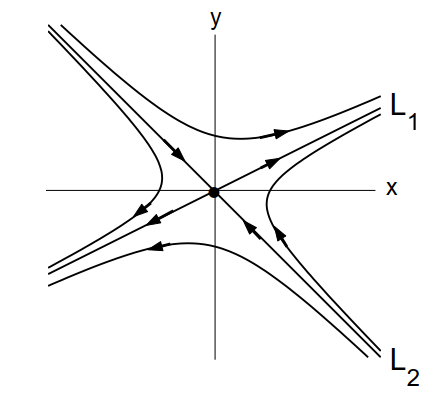
\includegraphics[width=100mm]{image/BT1/saddle.png}
    \end{center}
    
    
    \item $\lambda_1< \lambda _2<0$\\
    Loại phase portrait: Nodal Sink\\
   \begin{center}
        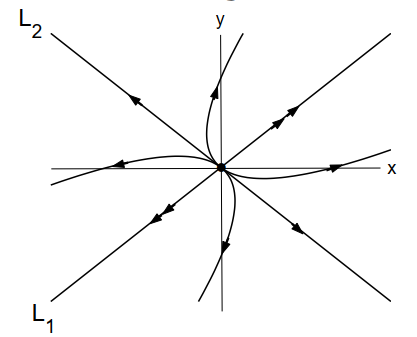
\includegraphics[width=100mm]{image/BT1/Nodal Sink.png}
   \end{center}
   
    
    \item $0<\lambda_1< \lambda _2$\\
    Loại phaseportrait: Nodal Source\\
    \begin{center}
        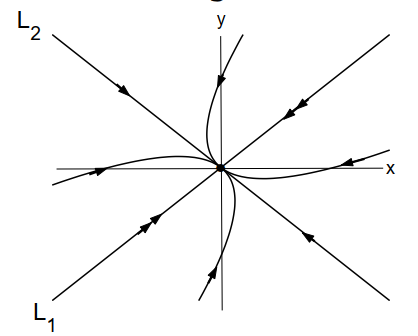
\includegraphics[width=100mm]{image/BT1/Nodal Source.png}
   \end{center}
\end{enumerate}
\textbf{Trường hợp 2:} phương trình $det(A-I \lambda)= 0$ có nghiệm phức có dạng $\lambda= m+i.n$.
\begin{enumerate}
    \item $m=0$\\
    Loại phaseportrait: Center
    \begin{center}
        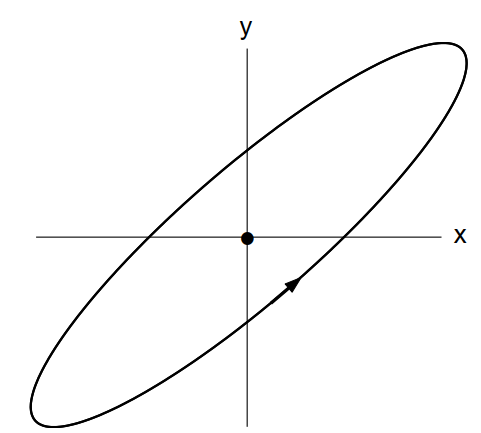
\includegraphics[width=100mm]{image/BT1/Center.png}
   \end{center}
    \item $m>0$\\
    Loại phaseportrait:  Spiral Source
    \begin{center}
        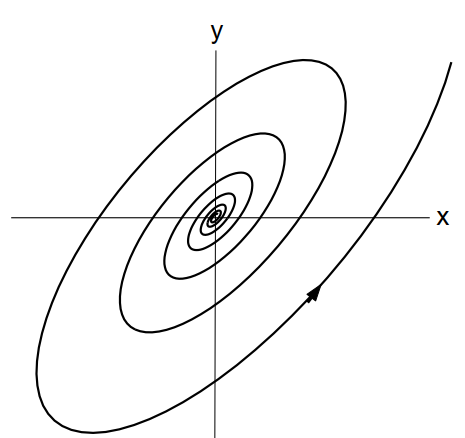
\includegraphics[width=100mm]{image/BT1/Spiral Source .png}
   \end{center}
    \item $m<0$\\
    Loại phaseportrait: Spiral Sink
    \begin{center}
        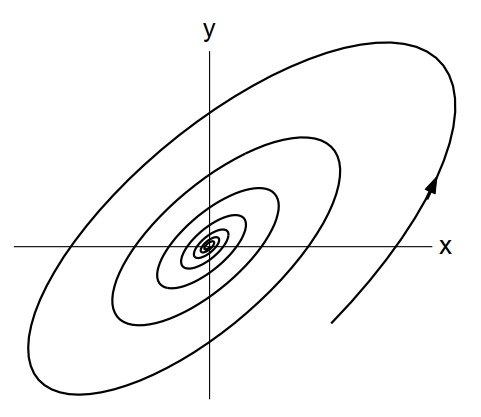
\includegraphics[width=100mm]{image/BT1/Spiral Sink.png}
   \end{center}
\end{enumerate}
\textbf{Trường hợp 3:} phương trình $det(A - I \lambda)=0$ có nghiệm kép $\lambda$.
\begin{enumerate}
    \item $\lambda >0$\\
    Loại phase portrait: Degenerate Nodal Source
    \begin{center}
        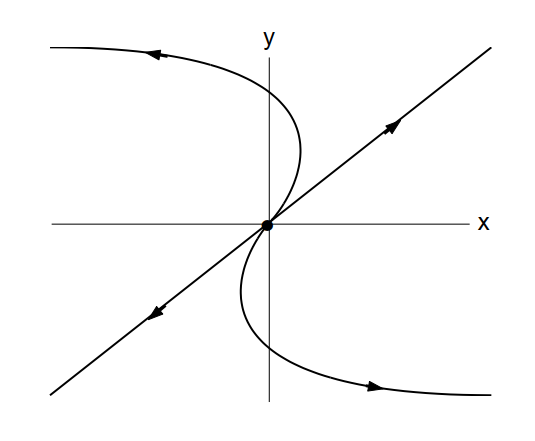
\includegraphics[width=100mm]{image/BT1/Degenerate Nodal Source.png}
   \end{center}
    \item $\lambda < 0$ \\
    Loại phase portrait: Degenerate Nodal Sink
    \begin{center}
        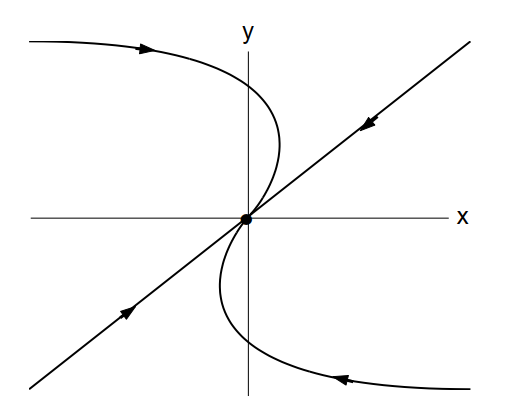
\includegraphics[width=100mm]{image/BT1/Degenerate Nodal Sink.png}
   \end{center}
    \item $\lambda = 0$ \\
    Loại phase portrait: Pure Shear
    \begin{center}
        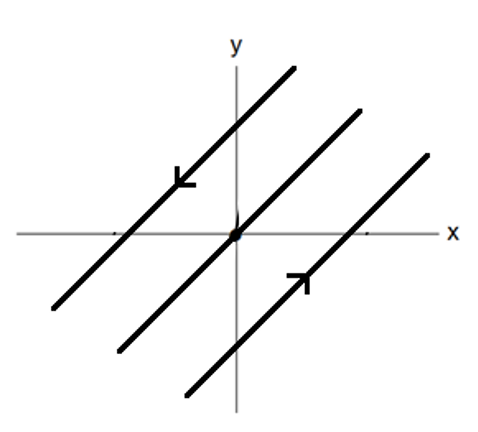
\includegraphics[width=100mm]{image/BT1/Pure Shear.png}
   \end{center}
\end{enumerate}
\textbf{Trường hợp 4:} phương trình $det(A - I \lambda)=0$ có hai nghiệm trong đó có một nghiệm bằng 0, một nghiệm khác 0. Đặt $\lambda$ là nghiệm khác 0  trong phương trình trên.
\begin{enumerate}
    \item $\lambda > 0$\\
    Loại phase portrait: Unstable Saddle-Node
    \begin{center}
        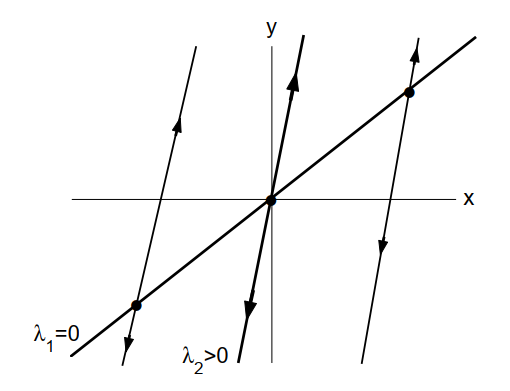
\includegraphics[width=100mm]{image/BT1/Unstable Saddle-Node.png}
   \end{center}
    \item $\lambda < 0$ \\
    Loại phase portrait: Stable Saddle-Node
    \begin{center}
        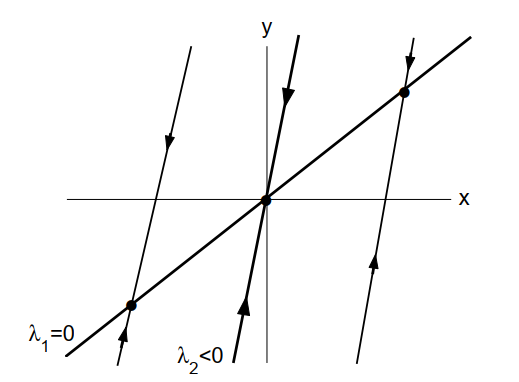
\includegraphics[width=100mm]{image/BT1/Stable Saddle-Node.png}
   \end{center}
\end{enumerate}
\begin{abstract}
    \begin{tabular}{|c|c|c|c|c|c|}
    \hline
       \textcolor{blue}{STT} & \textcolor{blue}{$Re \lambda_1$} &\textcolor{blue}{ $Re \lambda_2$} &  \textcolor{blue}{$\left | Im \lambda_1 \right |$ }& \textcolor{blue}{$\left | Im \lambda_2 \right |$} & \textcolor{blue}{Type}  \\ \hline
         \textcolor{blue}{1} & - & + & 0 & 0 & Saddle \\ \hline
         \textcolor{blue}{2} & - & - & 0 & 0 & Nodal Sink \\ \hline
         \textcolor{blue}{3} & + & + & 0 & 0 & Nodal Source \\ \hline
         \textcolor{blue}{4} & 0 & 0 & + & + & Center \\ \hline
         \textcolor{blue}{5} & + & + & + & + & Spiral Source \\ \hline
         \textcolor{blue}{6} & - & - & + & + & Spiral Sink \\ \hline
         \textcolor{blue}{7} & + & $=Re \lambda _1$ & 0 & 0 & Degenerate Nodal Source \\ \hline
         \textcolor{blue}{8} & - & $=Re \lambda _1$ & 0 & 0 & Degenerate Nodal Sink \\ \hline
         \textcolor{blue}{9} & 0 & 0 & 0 & 0 & Pure Shear \\ \hline
         \textcolor{blue}{10} & 0 & + & 0 & 0 & Unstable Saddle-Node \\ \hline
         \textcolor{blue}{11} & 0 & - & 0 & 0 & Stable Saddle-Node \\ 
         \hline
    \end{tabular}
\end{abstract}
\end{sol}


%%%%%%%%%%%%%%%%%%%%%%%%%%%%%%%%%%%%%%%%%%%%%%%
%%%%%%%%%%%%PROBLEM 2222222222222%%%%%%%%%%%%%%
%%%%%%%%%%%%%%%%%%%%%%%%%%%%%%%%%%%%%%%%%%%%%%%
	\pagebreak
\subsection{Bài tập 2} 

\begin{problem}
    For each combination of romantic styles in Tab. 1, give two concrete examples
of IVPs Sys. (3). Apply the formulae in Ex. 1 to find the exact solutions. Plot all the solutions and
the phase portraits.
\end{problem}
(Đây là link hiện thực bằng code python trên Google Collab của các ví dụ trong Bài tập này
\href{https://drive.google.com/drive/folders/1hVWgUYVexbeCH9ADyVudbC5ZGUV2hFjL?fbclid=IwAR20HoY8ihveweIgeqffKF-8PqHkPHfongm0XEFkxw2uM-Oj549LPzbs0ow}{Excercise 2} )
\begin{sol}

\subsubsection{Các kiểu kết hợp romatic styles và bảng ví dụ}
%%%%%%%%%%BẢNG VÍ DỤ%%%%%%%%%%%%%%%%%
\begin{table}[!htbp]
\begin{tabular}{|l|l|l|l|l|}
\hline
\textbf{TT} &
  \textbf{\begin{tabular}[c]{@{}l@{}}Romantic \\ style 1\end{tabular}} &
  \textbf{\begin{tabular}[c]{@{}l@{}}Romantic \\ style 2\end{tabular}} &
  \textbf{VD1} &
  \textbf{VD2} \\ \hline
1  & Eager Beaver      & Eager Beaver      &$\color{blue}\left\{\begin{matrix}
\dot{R} =  2R +3J \\ 
\dot{J} =  4R+2J\\ 
R(0)= -3, J(0)=-2
\end{matrix}\right.$  & $\color{blue}\left\{\begin{matrix}
\dot{R} =  3R + 2J \\ 
\dot{J} =  1R + 2J\\
R(0)= 3, J(0)=-2
\end{matrix}\right.$ \\ \hline
2  & Narcissistic Nerd & Narcissistic Nerd & $\color{blue}\left\{\begin{matrix}
\dot{R} =  2R -3J \\ 
\dot{J} =  -4R+3J\\ 
R(0)= 3, J(0)=-2
\end{matrix}\right.$ &$\color{blue}\left\{\begin{matrix}
\dot{R} =  4R + -4J \\ 
\dot{J} =  -4R + 4J\\ 
R(0)= \frac{5}{2}, J(0)=5
\end{matrix}\right.$  \\ \hline
3  & Cautious Lover    & Cautious Lover    & $\color{blue}\left\{\begin{matrix}
\dot{R} =  -3R + 4J \\ 
\dot{J} =  2R-5J\\ 
R(0)= - \frac{-3}{4}, J(0)=\frac{5}{4}
\end{matrix}\right.$ &  $\color{blue}\left\{\begin{matrix}
\dot{R} =  -\frac{5}{2}R + \frac{5}{2}J \\ 
\dot{J} =  3R -3J\\ 
R(0)= \frac{4}{5}, J(0)=\frac{9}{5}
\end{matrix}\right.$\\ \hline
4  & Hermit            & Hermit            & $\color{blue}\left\{\begin{matrix}
\dot{R} =  1R +6J \\ 
\dot{J} =  -3R+7J\\ 
R(0)= -3, J(0)=5
\end{matrix}\right.$ & $\color{blue}\left\{\begin{matrix}
\dot{R} =  -7R -9J \\ 
\dot{J} =  -4R -11J\\ 
R(0)= 3, J(0)=5
\end{matrix}\right.$ \\ \hline
5  & Eager Beaver      & Narcissistic Nerd & $\color{blue}\left\{\begin{matrix}
\dot{R} =  -3R -5J \\ 
\dot{J} =  -4R-2J\\ 
R(0)= -\frac{1}{6}, J(0)=\frac{3}{2}
\end{matrix}\right.$ & $\color{blue}\left\{\begin{matrix}
\dot{R} = 5R -2J \\ 
\dot{J} =  2R +1J\\ 
R(0)= \frac{9}{4}, J(0)=\frac{5}{4}
\end{matrix}\right.$ \\ \hline
6  & Eager Beaver      & Cautious Lover    & $\color{blue}\left\{\begin{matrix}
\dot{R} =  3R +J \\ 
\dot{J} =  2R-3J\\ 
R(0)= 2, J(0)=0
\end{matrix}\right.$ & $\color{blue}\left\{\begin{matrix}
\dot{R} = -2R +J \\ 
\dot{J} =  5R +2J\\ 
R(0)= -4, J(0)=2
\end{matrix}\right.$ \\ \hline
7  & Eager Beaver      & Hermit            & $\color{blue}\left\{\begin{matrix}
\dot{R} =  5R +10J \\ 
\dot{J} =  -5R-5J\\ 
R(0)= -\frac{7}{2}, J(0)=\frac{3}{2}
\end{matrix}\right.$ &  $\color{blue}\left\{\begin{matrix}
\dot{R} = -3R -2J \\ 
\dot{J} =  4R +J\\ 
R(0)= -\frac{12}{5}, J(0)=\frac{9}{4}
\end{matrix}\right.$\\ \hline
8  & Narcissistic Nerd & Cautious Lover    & $\color{blue}\left\{\begin{matrix}
\dot{R} =  2R -4J \\ 
\dot{J} =  R-2J\\ 
R(0)= -\frac{9}{2}, J(0)=3
\end{matrix}\right.$ & $\color{blue}\left\{\begin{matrix}
\dot{R} = 3R -4J \\ 
\dot{J} =  5R -J\\ 
R(0)= -2, J(0)=-3
\end{matrix}\right.$ \\ \hline
9  & Narcissistic Nerd & Hermit            & $\color{blue}\left\{\begin{matrix}
\dot{R} =  3R -2J \\ 
\dot{J} =  -3R-2J\\ 
R(0)= 4, J(0)=4
\end{matrix}\right.$ & $\color{blue}\left\{\begin{matrix}
\dot{R} = 2R -1J \\ 
\dot{J} =  -4R -2J\\ 
R(0)= -2, J(0)=1
\end{matrix}\right.$ \\ \hline
10 & Cautious Lover    & Hermit            & $\color{blue}\left\{\begin{matrix}
\dot{R} =  -2R +3J \\ 
\dot{J} =  -R-2J\\ 
R(0)= -\frac{12}{5}, J(0)=-\frac{9}{5}
\end{matrix}\right.$ &  $\color{blue}\left\{\begin{matrix}
\dot{R} = -6R -J \\ 
\dot{J} =  4R -2J\\ 
R(0)= -7, J(0)=4
\end{matrix}\right.$\\ \hline
\end{tabular}
\end{table}
%%%%%%%%%%END BẢNG VÍ DỤ%%%%%%%%%%%%%%%%%
\subsubsection{Giải các ví dụ và vẽ đồ thị}

\begin{tcbdoublebox}[title={1. Eager Beaver and Eager Beaver}]
\mdseries Giả sử với trường hợp cả hai nhân vật Romeo và Juliet đều là Eager Beaver. Theo định nghĩa, Eager Beaver là một người được thúc đẩy bởi cảm xúc của chính mình và bởi tình yêu của đối phương dành cho anh ấy/cô ấy. Nói cách khác, tình yêu của Romeo dành cho Juliet càng tăng khi Juliet cành yêu anh ta và chính anh ta cũng phải yêu Juliet. Đối với Juliet thì cũng tương tự vậy. Ở đây ta xét đến hai ví dụ IVP ODEs Sys:\\
\bfseries Ví dụ 1: \\
\textcolor{blue}{$$\left\{\begin{matrix}
\dot{R} =  2R +3J \\ 
\dot{J} =  4R+2J\\ 
R(0)= -3, J(0)=-2
\end{matrix}\right.$$}\\
\mdseries Ma trận $\color{blue}A=\begin{pmatrix}
2 & 3\\ 
4 & 2
\end{pmatrix}$ có hai trị riêng là 
$\color{blue}\lambda_{1}=2+2\sqrt{3};\ \lambda_{2}=2-2\sqrt{3}$
, lần lượt tương ứng với các vecto riêng:
$\color{blue}v_{1} = (\sqrt{3}; 2)^{T};\ v_{2}=(\sqrt{3}; -2)^{T}$\\Áp dụng công thức bài tập 1, nghiệm của hệ phương trình là:
$$R(t)=-\frac{{\mathrm{e}}^{2\,t\,\left(\sqrt{3}+1\right)}\,\left(\sqrt{3}+3\right)}{2}-\frac{\sqrt{3}\,{\mathrm{e}}^{-2\,t\,\left(\sqrt{3}-1\right)}\,\left(\sqrt{3}-1\right)}{2} $$
$$J(t)={\mathrm{e}}^{-2\,t\,\left(\sqrt{3}-1\right)}\,\left(\sqrt{3}-1\right)-\frac{\sqrt{3}\,{\mathrm{e}}^{2\,t\,\left(\sqrt{3}+1\right)}\,\left(\sqrt{3}+3\right)}{3}$$
\\
\bfseries Ví dụ 2: \\
$$\color{blue}\left\{\begin{matrix}
\dot{R} =  3R + 2J \\ 
\dot{J} =  1R + 2J\\
R(0)= 3, J(0)=-2
\end{matrix}\right.$$
\mdseries Ma trận $\color{blue}A=\begin{pmatrix}
3 & 2\\ 
1 & 2
\end{pmatrix}$ có hai trị riêng lần lượt là $\color{blue}\lambda_{1}=4;\ \lambda_{2}=1$
, lần lượt tương ứng với các vecto riêng:
$\color{blue}v_{1} = (2;\ 1)^{T};\ v_{2}=(-1;\ 1)^{T}$
\\
Áp dụng công thức bài tập 1, nghiệm của hệ phương trình là:
$$R(t)=\frac{2\,{\mathrm{e}}^{4\,t}}{3}+\frac{7\,{\mathrm{e}}^t}{3} $$
$$J(t)=\frac{{\mathrm{e}}^{4\,t}}{3}-\frac{7\,{\mathrm{e}}^t}{3}$$

\textbf{Nhận xét: } Như đã nói, vì cả hai đều là Eager Beaver, nên tình cảm của cả hai sẽ phụ thuộc vào chính họ và đối phương. Thế nên trong \textbf{Ví dụ 1} khi mà thời điểm ban đầu cả hai đều ghét nhau thì theo thời gian tình cảm của họ sẽ ngày càng giảm đi, còn trong \textbf{Ví dụ 2} ban đầu dù có một bên ghét thế nhưng các chỉ số a,b,c,d sẽ kéo tình cảm này lên dương vào một thời điểm nào đó và khi thời gian đủ lớn, tình cảm cả hai cũng ngày càng tăng lên. 

Hai cặp \textbf{đồ thị plot và phase portrait} dưới đây sẽ mô tả cho điều này!
\end{tcbdoublebox}
\pagebreak
\begin{figure}[!htbp]
    \centering
    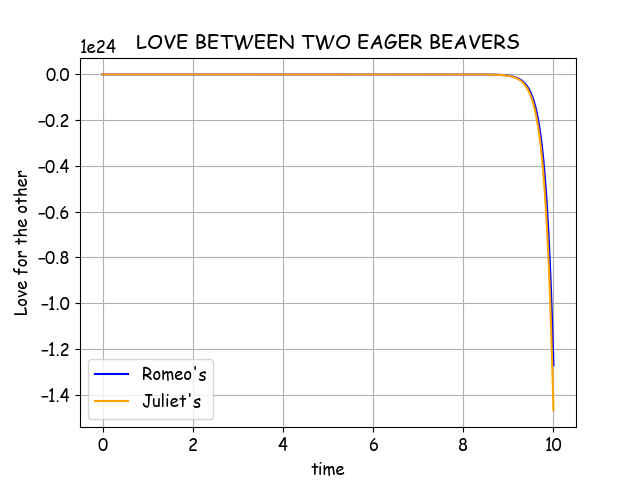
\includegraphics[width=100mm]{image/bt2/plot1.1.png}
    \caption{VD1.1 - The plot of the love between two eager beavers }
\end{figure}
\begin{figure}[!htbp]
    \centering
    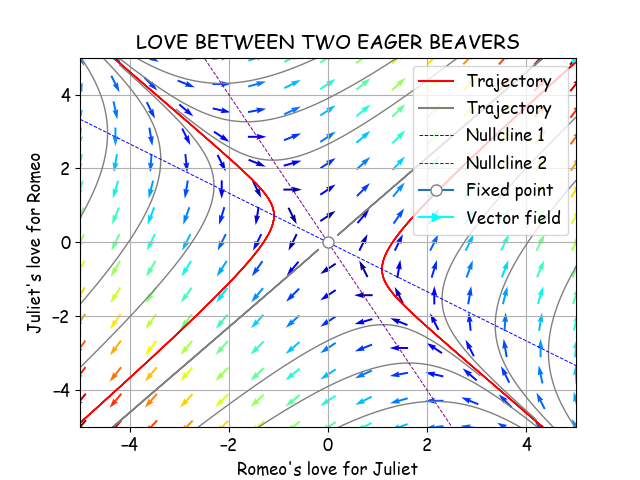
\includegraphics[width=100mm]{image/bt2/pp1.1.png}
    \caption{VD1.1 - The phase portrait of the love between two eager beavers}
\end{figure}

\textbf{Dạng Phase portrait: } Saddle
\pagebreak
\begin{figure}[!htbp]
    \centering
    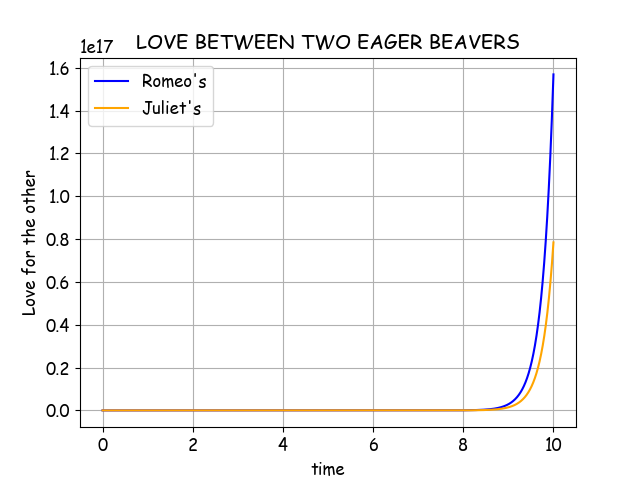
\includegraphics[width=100mm]{image/bt2/plot1.2.png}
    \caption{VD1.2 - The plot of the love between two eager beavers}
\end{figure}
\begin{figure}[!htbp]
    \centering
    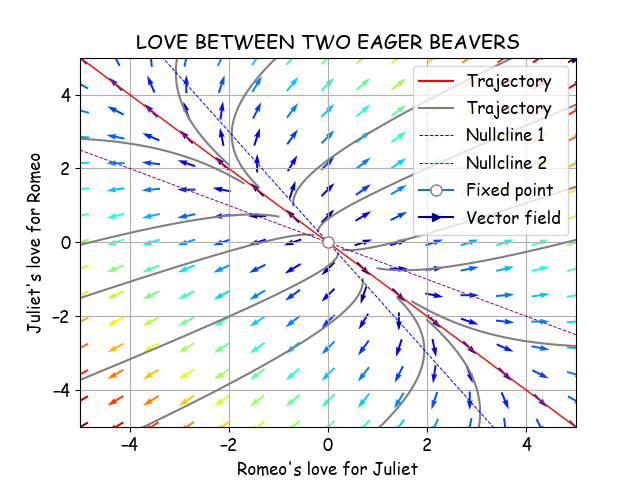
\includegraphics[width=100mm]{image/bt2/pp1.2.png}
    \caption{VD1.2 - The phase portrait of the love between two eager beavers}
\end{figure}

\textbf{Dạng Phase portrait: } Nodal Source
\pagebreak

%%%%%%%%%%%%%%%%%%2222222222%%%%%%%%%%%%%%%%%%%%%%%%
%%%%%%%%%%%%%%%%%%%%%%%%%%%%%%%%%%%%%%%%%%%%%%%%%%%%%
\begin{tcbdoublebox}[title={2. Narcissistic Nerd and Narcissistic Nerd}]
\mdseries .\\
\bfseries Ví dụ 1: \\
\textcolor{blue}{$$\left\{\begin{matrix}
\dot{R} =  2R -3J \\ 
\dot{J} =  -4R+3J\\ 
R(0)= 3, J(0)=-2
\end{matrix}\right.$$}\\
\mdseries Ma trận $\color{blue}A=\begin{pmatrix}
2 & -3\\ 
-4 & 3
\end{pmatrix}$ có hai trị riêng là 
$\color{blue}\lambda_{1}=-1;\ \lambda_{2}=6$
, lần lượt tương ứng với các vecto riêng:
$\color{blue}v_{1} = (1;\ 1)^{T};\ v_{2}=(-3;\ 4)^{T}$\\Áp dụng công thức bài tập 1, nghiệm của hệ phương trình là:
$$R(t)=\frac{6\,{\mathrm{e}}^{-t}}{7}+\frac{15\,{\mathrm{e}}^{6\,t}}{7} $$
$$J(t)=\frac{6\,{\mathrm{e}}^{-t}}{7}-\frac{20\,{\mathrm{e}}^{6\,t}}{7}$$
\\
\bfseries Ví dụ 2:\\
\textcolor{blue}{$$\left\{\begin{matrix}
\dot{R} =  4R + -4J \\ 
\dot{J} =  -4R + 4J\\ 
R(0)= \frac{5}{2}, J(0)=5
\end{matrix}\right.$$}
\mdseries Ma trận $\color{blue}A=\begin{pmatrix}
4 & -4\\ 
-4 & 4
\end{pmatrix}$ có hai trị riêng là 
$\color{blue}\lambda_{1}=0;\ \lambda_{2}=8$
, lần lượt tương ứng với các vecto riêng:
$\color{blue}v_{1} = (1;\ 1)^{T};\ v_{2}=(-1;\ 1)^{T}$\\Áp dụng công thức bài tập 1, nghiệm của hệ phương trình là:
$$R(t)=\frac{15}{4}-\frac{5\,{\mathrm{e}}^{8\,t}}{4}$$
$$J(t)=\frac{5\,{\mathrm{e}}^{8\,t}}{4}+\frac{15}{4}$$

\textbf{Nhận xét: } Trong trường hợp này, cả Romeo và Juliet đều là Narcissistic Nerd. Theo định nghĩa, Narcissistic Nerd là người có xu hướng thể hiện ngược lại tình cảm của phía đối phương dành cho mình và bị khuyến khích bởi tình cảm của mình. Trong \textbf{Ví dụ 1}, ta thấy rằng khi thời gian t đủ lớn, tình cảm của Romeo có xu hướng tăng lên, vì vậy theo như phong cách
của mình thì tình yêu của Juliet sẽ giảm xuống và cô ấy có xu hướng ghét Romeo nhiều hơn, còn trong \textbf{Ví dụ 2} thì ngược lại!

Hai cặp \textbf{đồ thị plot và phase portrait} dưới đây sẽ mô tả cho điều này!
\end{tcbdoublebox}
\pagebreak
\begin{figure}[!htbp]
    \centering
    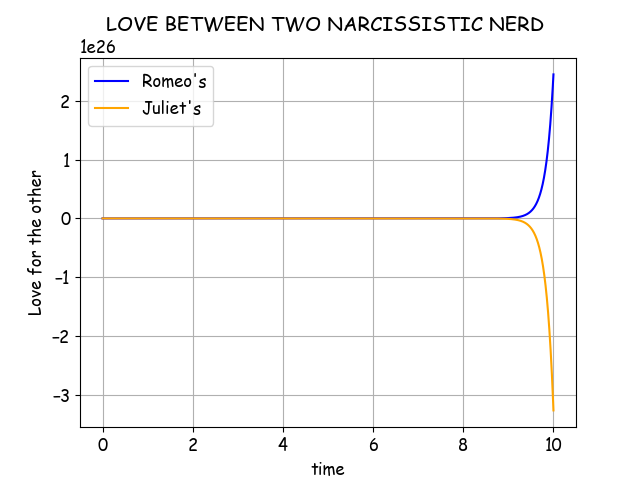
\includegraphics[width=100mm]{image/bt2/plot2.1.png}
    \caption{VD2.1 - The plot of the love between two Narcissistic Nerd }
\end{figure}

\textbf{Dạng Phase portrait: } Saddle
\begin{figure}[!htbp]
    \centering
    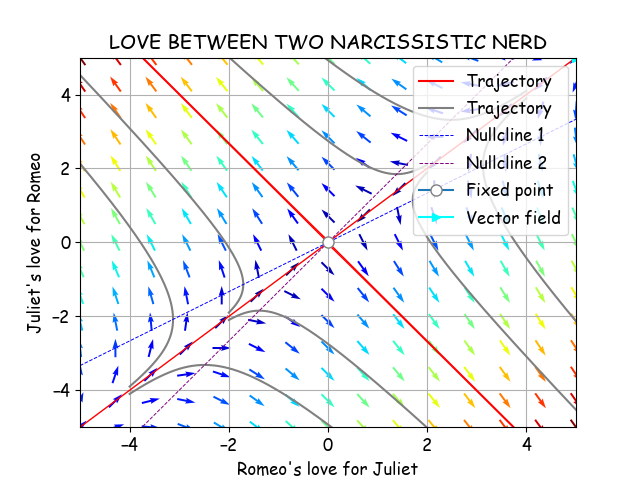
\includegraphics[width=100mm]{image/bt2/pp2.1.png}
    \caption{VD2.1 - The phase portrait of the love between two Narcissistic Nerd}
\end{figure}
\pagebreak
\begin{figure}[!htbp]
    \centering
    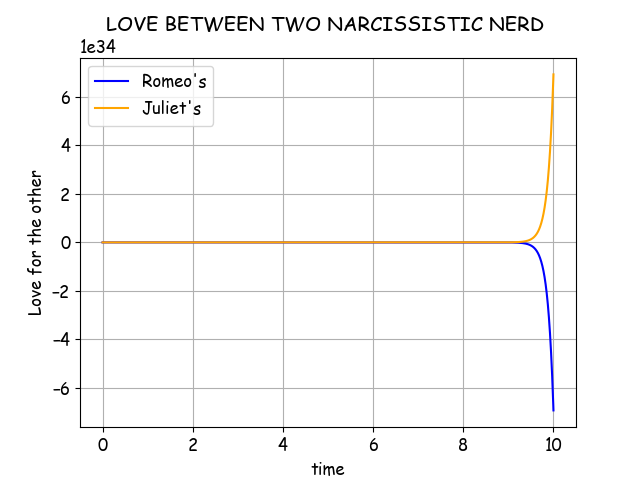
\includegraphics[width=100mm]{image/bt2/plot2.2.png}
    \caption{VD2.2 - The plot of the love between two Narcissistic Nerd}
\end{figure}
\begin{figure}[!htbp]
    \centering
    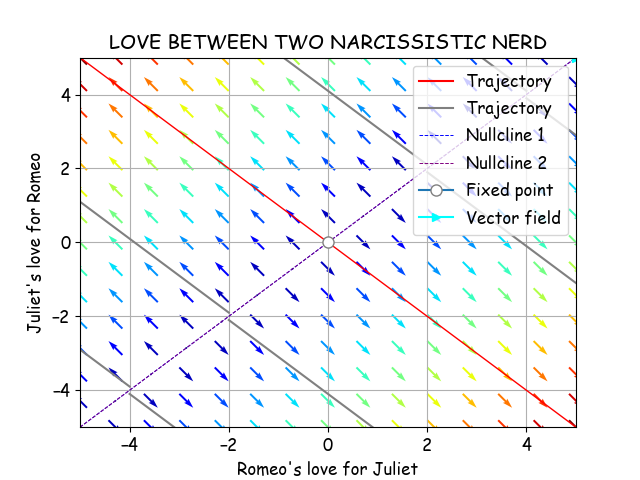
\includegraphics[width=100mm]{image/bt2/pp2.2.png}
    \caption{VD2.2 - The phase portrait of the love between two Narcissistic Nerd}
\end{figure}

\textbf{Dạng Phase portrait: } Unstable Saddle-Node
\pagebreak
%%%%%%%%%%%%%%%%%%33333333333%%%%%%%%%%%%%%%%%%%%%%%%
%%%%%%%%%%%%%%%%%%%%%%%%%%%%%%%%%%%%%%%%%%%%%%%%%%%%%
\begin{tcbdoublebox}[title={3. Cautious Lover and Cautious Lover}]
\mdseries .\\
\bfseries Ví dụ 1: \\
\textcolor{blue}{$$\left\{\begin{matrix}
\dot{R} =  -3R + 4J \\ 
\dot{J} =  2R-5J\\ 
R(0)= - \frac{-3}{4}, J(0)=\frac{5}{4}
\end{matrix}\right.$$}\\
\mdseries Ma trận $\color{blue}A=\begin{pmatrix}
-3 & 4\\ 
2 & -5
\end{pmatrix}$ có hai trị riêng là 
$\color{blue}\lambda_{1}=-1;\ \lambda_{2}=-7$
, lần lượt tương ứng với các vecto riêng:
$\color{blue}v_{1} = (2;\ 1)^{T};\ v_{2}=(-1;\ 1)^{T}$\\Áp dụng công thức bài tập 1, nghiệm của hệ phương trình là:
$$R(t)=\frac{{\mathrm{e}}^{-t}}{3}-\frac{13\,{\mathrm{e}}^{-7\,t}}{12} $$
$$J(t)=\frac{{\mathrm{e}}^{-t}}{6}+\frac{13\,{\mathrm{e}}^{-7\,t}}{12}$$
\\
\bfseries Ví dụ 2:\\
\textcolor{blue}{$$\left\{\begin{matrix}
\dot{R} =  -\frac{5}{2}R + \frac{5}{2}J \\ 
\dot{J} =  3R -3J\\ 
R(0)= \frac{4}{5}, J(0)=\frac{9}{5}
\end{matrix}\right.$$}
\mdseries Ma trận $\color{blue}A=\begin{pmatrix}
-\frac{5}{2} & \frac{5}{2}\\ 
3 & -3
\end{pmatrix}$ có hai trị riêng là 
$\color{blue}\lambda_{1}=0;\ \lambda_{2}=-\frac{11}{2}$
, lần lượt tương ứng với các vecto riêng:
$\color{blue}v_{1} = (1;\ 1)^{T};\ v_{2}=(-\frac{5}{6};\ 1)^{T}$\\Áp dụng công thức bài tập 1, nghiệm của hệ phương trình là:
$$R(t)=\frac{69}{55}-\frac{5\,{\mathrm{e}}^{-\frac{11\,t}{2}}}{11}$$
$$J(t)=\frac{6\,{\mathrm{e}}^{-\frac{11\,t}{2}}}{11}+\frac{69}{55}$$

\textbf{Nhận xét: } Trong trường hợp này, cả Romeo và Juliet đều là Cautious Lover. Theo định nghĩa, Cautious Lover có xu hướng không bị khuyến khích bởi tình cảm của mình và phản ứng với tình cảm của đối phương. Trong \textbf{Ví dụ 1}, ta thấy rằng, ban đầu có người thích có người ghét đối phương, vì vậy theo thời gian thì tình cảm của 2 người sẽ dần tiến tới 0, còn trong \textbf{Ví dụ 2} sẽ tiến tới một hằng số nhất định bởi ban đầu cả hai đều có tình ý với đối phương.

Hai cặp \textbf{đồ thị plot và phase portrait} dưới đây sẽ mô tả cho điều này!
\end{tcbdoublebox}
\pagebreak
\begin{figure}[!htbp]
    \centering
    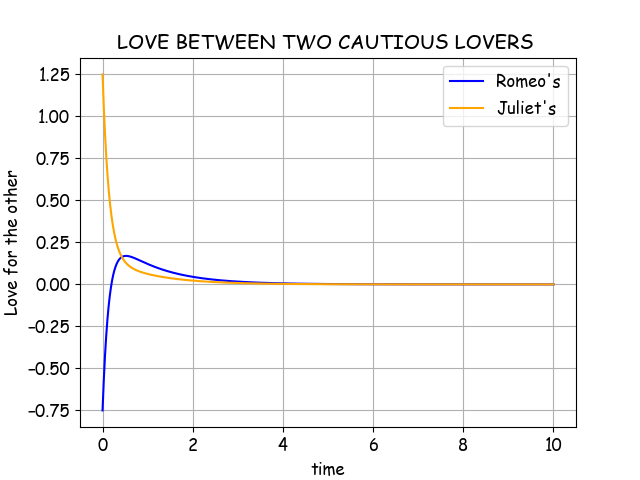
\includegraphics[width=100mm]{image/bt2/plot3.1.png}
    \caption{VD3.1 - The plot of the love between two Cautious Lovers }
\end{figure}
\begin{figure}[!htbp]
    \centering
    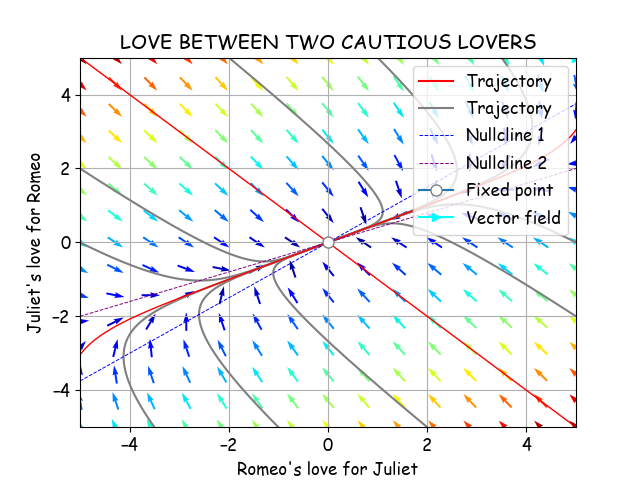
\includegraphics[width=100mm]{image/bt2/pp3.1.png}
    \caption{VD3.1 - The phase portrait of the love between two Cautious Lovers}
\end{figure}

\textbf{Dạng Phase portrait: } Nodal Sink
\pagebreak
\begin{figure}[!htbp]
    \centering
    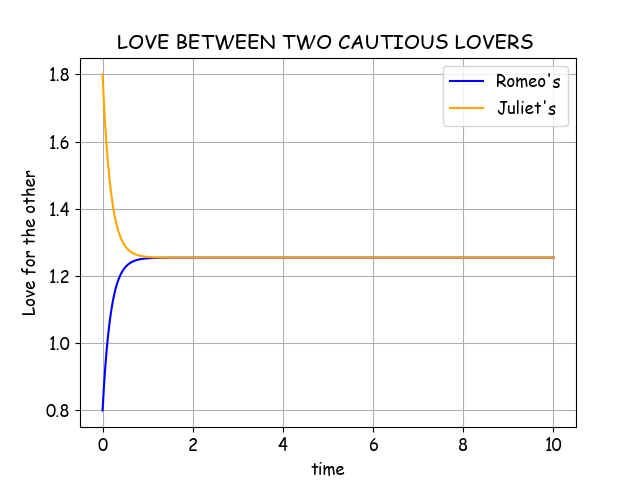
\includegraphics[width=100mm]{image/bt2/plot3.2.png}
    \caption{VD3.2 - The plot of the love between two Cautious Lovers}
\end{figure}
\begin{figure}[!htbp]
    \centering
    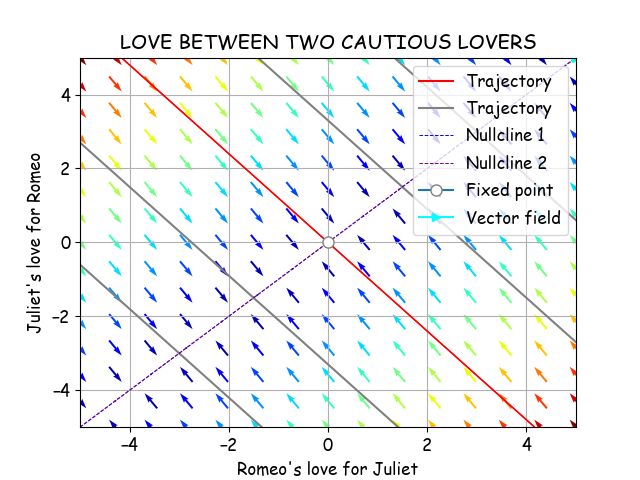
\includegraphics[width=100mm]{image/bt2/pp3.2.png}
    \caption{VD3.2 - The phase portrait of the love between two Cautious Lovers}
\end{figure}

\textbf{Dạng Phase portrait: } Stable Saddle-Node
\pagebreak
%%%%%%%%%%%%%%%%%%44444444444%%%%%%%%%%%%%%%%%%%%%%%%
%%%%%%%%%%%%%%%%%%%%%%%%%%%%%%%%%%%%%%%%%%%%%%%%%%%%%
\begin{tcbdoublebox}[title={4. Hermit and Hermit}]
\mdseries .\\
\bfseries Ví dụ 1: \\
\textcolor{blue}{$$\left\{\begin{matrix}
\dot{R} =  -3R -5J \\ 
\dot{J} =  -4R-2J\\ 
R(0)= -\frac{1}{6}, J(0)=\frac{3}{2}
\end{matrix}\right.$$}\\
\mdseries Ma trận $\color{blue}A=\begin{pmatrix}
-3 & -5\\ 
-4 & -2
\end{pmatrix}$ có hai trị riêng là 
$\color{blue}\lambda_{1}=-7;\ \lambda_{2}=2$
, lần lượt tương ứng với các vecto riêng:
$\color{blue}v_{1} = (5;\ 4)^{T};\ v_{2}=(-1;\ 1)^{T}$\\Áp dụng công thức bài tập 1, nghiệm của hệ phương trình là:
$$R(t)=\frac{20\,{\mathrm{e}}^{-7\,t}}{27}-\frac{49\,{\mathrm{e}}^{2\,t}}{54} $$
$$J(t)=\frac{49\,{\mathrm{e}}^{2\,t}}{54}+\frac{16\,{\mathrm{e}}^{-7\,t}}{27}$$
\\
\bfseries Ví dụ 2:\\
\textcolor{blue}{$$\left\{\begin{matrix}
\dot{R} =  -7R -9J \\ 
\dot{J} =  -4R -11J\\ 
R(0)= 3, J(0)=5
\end{matrix}\right.$$}
\mdseries Ma trận $\color{blue}A=\begin{pmatrix}
-7 & -9\\ 
-4 & -11
\end{pmatrix}$ có hai trị riêng là 
$\color{blue}\lambda_{1}=-9+2\sqrt{10};\ \lambda_{2}=-9-2\sqrt{10}$
, lần lượt tương ứng với các vecto riêng:
$\color{blue}v_{1} = (-1-\sqrt{10};\ 2)^{T};\ v_{2}=(-1+\sqrt{10};\ 2)^{T}$\\Áp dụng công thức bài tập 1, nghiệm của hệ phương trình là:
$$R(t)={\mathrm{e}}^{t\,\left(2\,\sqrt{10}-9\right)}\,\left(\frac{\sqrt{10}}{2}+\frac{1}{2}\right)\,\left(\frac{11\,\sqrt{10}}{20}-\frac{5}{2}\right)+\frac{\sqrt{10}\,{\mathrm{e}}^{-t\,\left(2\,\sqrt{10}+9\right)}\,\left(\frac{\sqrt{10}}{2}-\frac{1}{2}\right)\,\left(5\,\sqrt{10}+11\right)}{20}$$
$$J(t)=\frac{\sqrt{10}\,{\mathrm{e}}^{-t\,\left(2\,\sqrt{10}+9\right)}\,\left(5\,\sqrt{10}+11\right)}{20}-{\mathrm{e}}^{t\,\left(2\,\sqrt{10}-9\right)}\,\left(\frac{11\,\sqrt{10}}{20}-\frac{5}{2}\right)$$

\textbf{Nhận xét: } Trong trường hợp này, cả Romeo và Juliet đều là Hermit. Theo định nghĩa, Hermit sẽ có xu hướng không bị khuyến khích bởi tình cảm của bản thân
cũng như đối phương. Trong \textbf{Ví dụ 1}, , còn trong \textbf{Ví dụ 2} ban đầu ta thấy cả 2 người đều thích nhau, tuy nhiên vì họ là Hermit nên
ban đầu tình cảm của họ giảm dần và giữ nguyên khi thời gian tăng lên.

Hai cặp \textbf{đồ thị plot và phase portrait} dưới đây sẽ mô tả cho điều này!
\end{tcbdoublebox}
\pagebreak
\begin{figure}[!htbp]
    \centering
    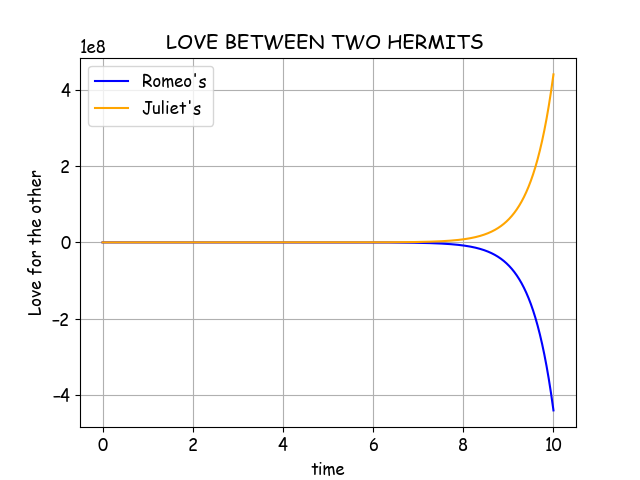
\includegraphics[width=100mm]{image/bt2/plot4.1.png}
    \caption{VD4.1 - The plot of the love between two Hermits }
\end{figure}
\begin{figure}[!htbp]
    \centering
    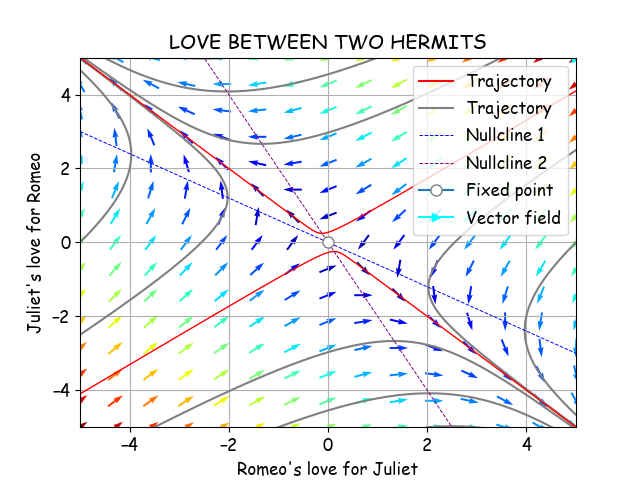
\includegraphics[width=100mm]{image/bt2/pp4.1.png}
    \caption{VD4.1 - The phase portrait of the love between two Hermits}
\end{figure}

\textbf{Dạng Phase portrait: } Saddle
\pagebreak
\begin{figure}[!htbp]
    \centering
    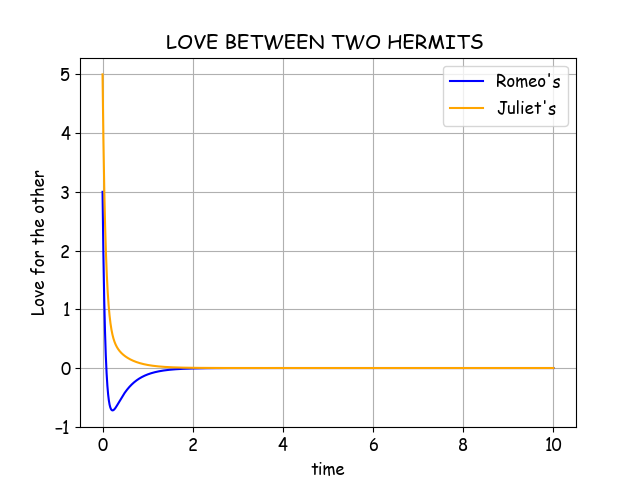
\includegraphics[width=100mm]{image/bt2/plot4.2.png}
    \caption{VD4.2 - The plot of the love between two Hermits}
\end{figure}
\begin{figure}[!htbp]
    \centering
    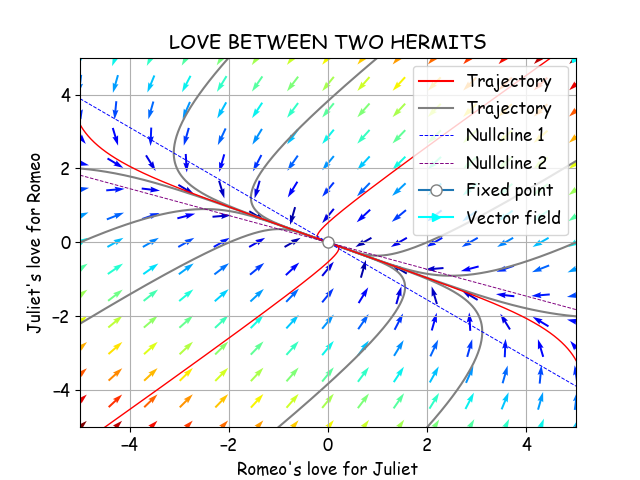
\includegraphics[width=100mm]{image/bt2/pp4.2.png}
    \caption{VD4.2 - The phase portrait of the love between two Hermits}
\end{figure}

\textbf{Dạng Phase portrait: } Spiral Sink
\pagebreak
%%%%%%%%%%%%%%%%%%55555555555%%%%%%%%%%%%%%%%%%%%%%%%
%%%%%%%%%%%%%%%%%%%%%%%%%%%%%%%%%%%%%%%%%%%%%%%%%%%%%
\begin{tcbdoublebox}[title={5. Eager Beaver and Narcissistic Nerd}]
\mdseries .\\
\bfseries Ví dụ 1: \\
\textcolor{blue}{$$\left\{\begin{matrix}
\dot{R} =  1R +6J \\ 
\dot{J} =  -3R+7J\\ 
R(0)= -3, J(0)=5
\end{matrix}\right.$$}\\
\mdseries Ma trận $\color{blue}A=\begin{pmatrix}
1 & 6\\ 
-3 & 7
\end{pmatrix}$ có hai trị riêng là 
$\color{blue}\lambda_{1}=4+3i;\ \lambda_{2}=4-3i$
, lần lượt tương ứng với các vecto riêng:
$\color{blue}v_{1} = (1-i;\ 1)^{T};\ v_{2}=(1+i;\ 1)^{T}$\\Áp dụng công thức bài tập 1, nghiệm của hệ phương trình là:
$$R(t)=3\,\cos\left(3\,t\right)\,{\mathrm{e}}^{4\,t}+7\,\sin\left(3\,t\right)\,{\mathrm{e}}^{4\,t} $$
$$J(t)=5\,\cos\left(3\,t\right)\,{\mathrm{e}}^{4\,t}+2\,\sin\left(3\,t\right)\,{\mathrm{e}}^{4\,t}$$
\\
\bfseries Ví dụ 2:\\
\textcolor{blue}{$$\left\{\begin{matrix}
\dot{R} = 5R -2J \\ 
\dot{J} =  2R +1J\\ 
R(0)= \frac{9}{4}, J(0)=\frac{5}{4}
\end{matrix}\right.$$}
\mdseries Ma trận $\color{blue}A=\begin{pmatrix}
5 & -2\\ 
2 & 1
\end{pmatrix}$ có trị riêng bội 2 là 
$\color{blue}\lambda_{1}=\lambda_{2}=3$ tương ứng với vecto riêng:
$\color{blue}v_{1} = v_{2}=(1;\ 1)^{T}$\\Áp dụng công thức bài tập 1, nghiệm của hệ phương trình là:
$$R(t)=\frac{9\,{\mathrm{e}}^{3\,t}}{4}+2\,t\,{\mathrm{e}}^{3\,t}$$
$$J(t)=\frac{5\,{\mathrm{e}}^{3\,t}}{4}+2\,t\,{\mathrm{e}}^{3\,t}$$

\end{tcbdoublebox}
\pagebreak
\begin{figure}[!htbp]
    \centering
    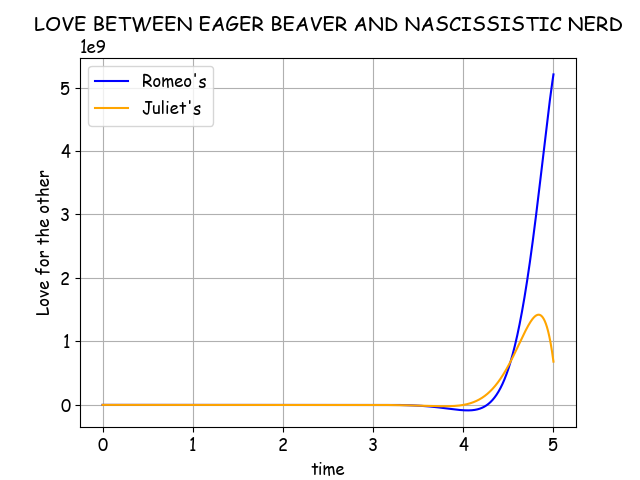
\includegraphics[width=100mm]{image/bt2/plot5.1.png}
    \caption{VD5.1 - The plot of the love between Eager Beaver and Narcissistic Nerd}
\end{figure}
\begin{figure}[!htbp]
    \centering
    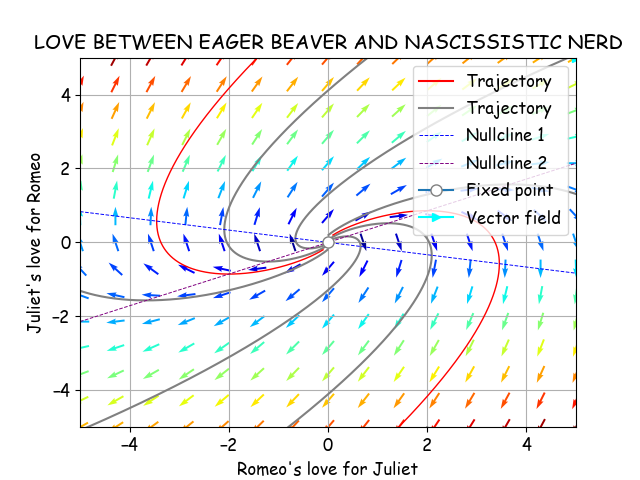
\includegraphics[width=100mm]{image/bt2/pp5.1.png}
    \caption{VD5.1 - The phase portrait of the love between Eager Beaver and Narcissistic Nerd}
\end{figure}

\textbf{Dạng Phase portrait: } Spiral Source
\pagebreak
\begin{figure}[!htbp]
    \centering
    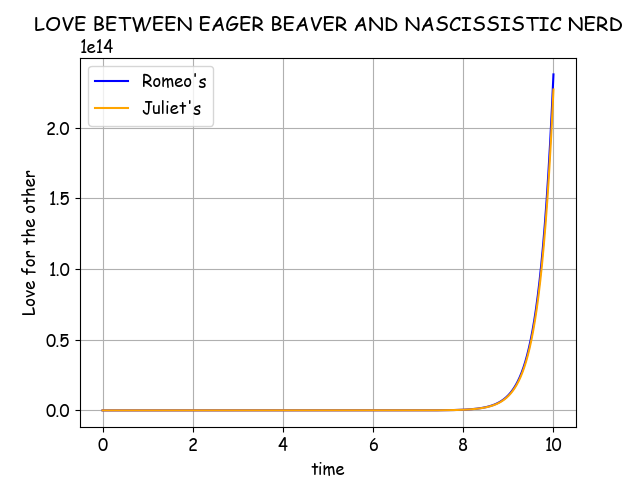
\includegraphics[width=100mm]{image/bt2/plot5.2.png}
    \caption{VD5.2 - The plot of the love between Eager Beaver and Narcissistic Nerd}
\end{figure}
\begin{figure}[!htbp]
    \centering
    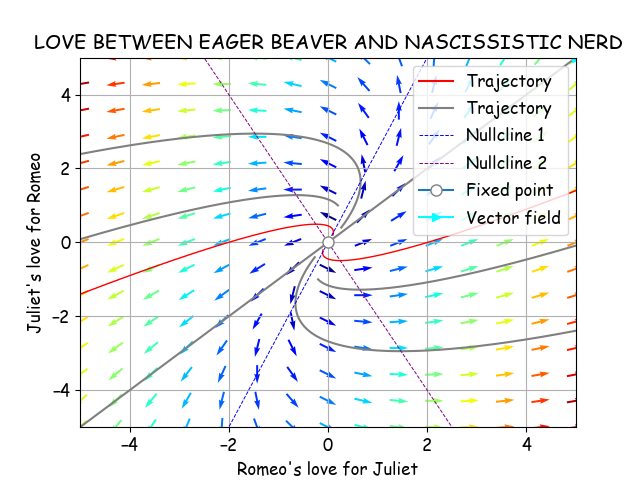
\includegraphics[width=100mm]{image/bt2/pp5.2.png}
    \caption{VD5.2 - The phase portrait of the love between Eager Beaver and Narcissistic Nerd}
\end{figure}

\textbf{Dạng Phase portrait: } Degenerate Nodal Source
\pagebreak
%%%%%%%%%%%%%%%%%%666666666666%%%%%%%%%%%%%%%%%%%%%%%%
%%%%%%%%%%%%%%%%%%%%%%%%%%%%%%%%%%%%%%%%%%%%%%%%%%%%%
\begin{tcbdoublebox}[title={6. Eager Beaver and Cautious Lover}]
\mdseries .\\
\bfseries Ví dụ 1: \\
\textcolor{blue}{$$\left\{\begin{matrix}
\dot{R} =  3R +J \\ 
\dot{J} =  2R-3J\\ 
R(0)= 2, J(0)=0
\end{matrix}\right.$$}\\
\mdseries Ma trận $\color{blue}A=\begin{pmatrix}
-3 & -5\\ 
-4 & -2
\end{pmatrix}$ có hai trị riêng là 
$\color{blue}\lambda_{1}=-\sqrt{11};\ \lambda_{2}=\sqrt{11}$
, lần lượt tương ứng với các vecto riêng:
$\color{blue}v_{1} = (3-\sqrt{11};\ 2)^{T};\ v_{2}=(3+\sqrt{11};\ 2)^{T}$\\Áp dụng công thức bài tập 1, nghiệm của hệ phương trình là:
$$R(t)=\frac{2\,\sqrt{11}\,{\mathrm{e}}^{\sqrt{11}\,t}\,\left(\frac{\sqrt{11}}{2}+\frac{3}{2}\right)}{11}+\frac{2\,\sqrt{11}\,{\mathrm{e}}^{-\sqrt{11}\,t}\,\left(\frac{\sqrt{11}}{2}-\frac{3}{2}\right)}{11}$$
$$J(t)=\frac{2\,\sqrt{11}\,{\mathrm{e}}^{\sqrt{11}\,t}}{11}-\frac{2\,\sqrt{11}\,{\mathrm{e}}^{-\sqrt{11}\,t}}{11}$$
\\
\bfseries Ví dụ 2:\\
\textcolor{blue}{$$\left\{\begin{matrix}
\dot{R} = -2R +J \\ 
\dot{J} =  5R +2J\\ 
R(0)= -4, J(0)=2
\end{matrix}\right.$$}
\mdseries Ma trận $\color{blue}A=\begin{pmatrix}
-2 & 1\\ 
5 & 2
\end{pmatrix}$ có hai trị riêng là 
$\color{blue}\lambda_{1}=3;\ \lambda_{2}=-3$
, lần lượt tương ứng với các vecto riêng:
$\color{blue}v_{1} = (1;\ 5)^{T};\ v_{2}=(-1;\ 1)^{T}$\\Áp dụng công thức bài tập 1, nghiệm của hệ phương trình là:
$$R(t)=-\frac{11\,{\mathrm{e}}^{-3\,t}}{3}-\frac{{\mathrm{e}}^{3\,t}}{3}$$
$$J(t)=\frac{11\,{\mathrm{e}}^{-3\,t}}{3}-\frac{5\,{\mathrm{e}}^{3\,t}}{3}$$

\end{tcbdoublebox}
\pagebreak
\begin{figure}[!htbp]
    \centering
    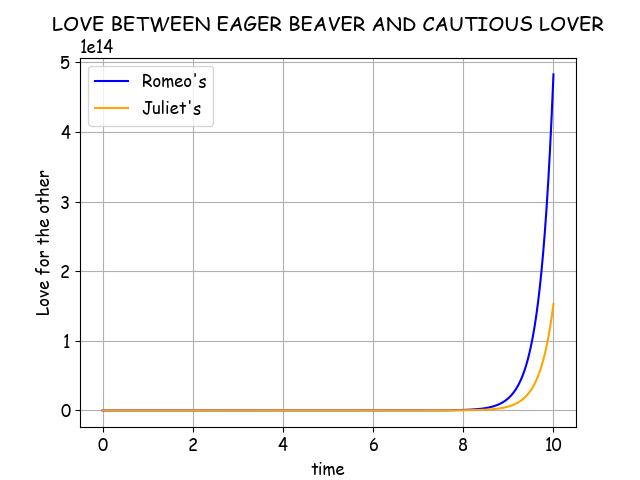
\includegraphics[width=100mm]{image/bt2/plot6.1.png}
    \caption{VD6.1 - The plot of the love between Eager Beaver and Cautious Lover}
\end{figure}
\begin{figure}[!htbp]
    \centering
    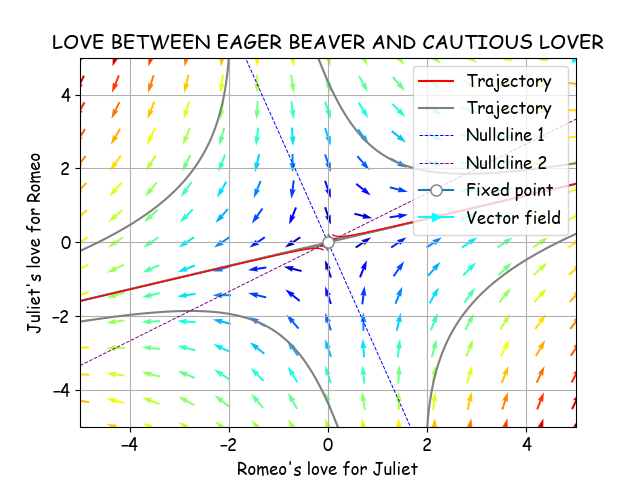
\includegraphics[width=100mm]{image/bt2/pp6.1.png}
    \caption{VD6.1 - The phase portrait of the love between Eager Beaver and Cautious Lover}
\end{figure}

\textbf{Dạng Phase portrait: } Saddle
\pagebreak
\begin{figure}[!htbp]
    \centering
    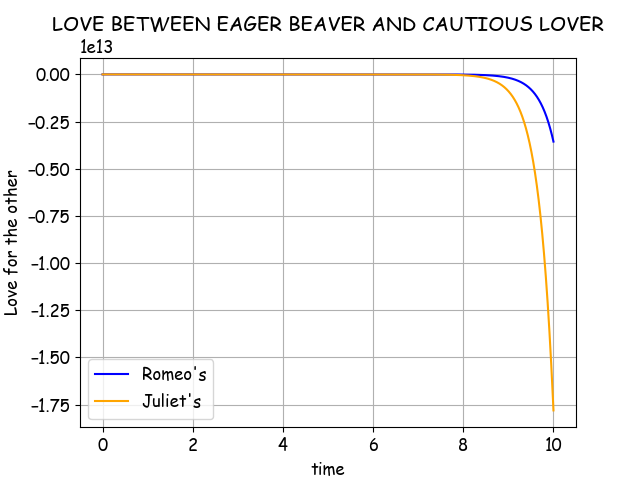
\includegraphics[width=100mm]{image/bt2/plot6.2.png}
    \caption{VD6.2 - The plot of the love between Eager Beaver and Cautious Lover}
\end{figure}
\begin{figure}[!htbp]
    \centering
    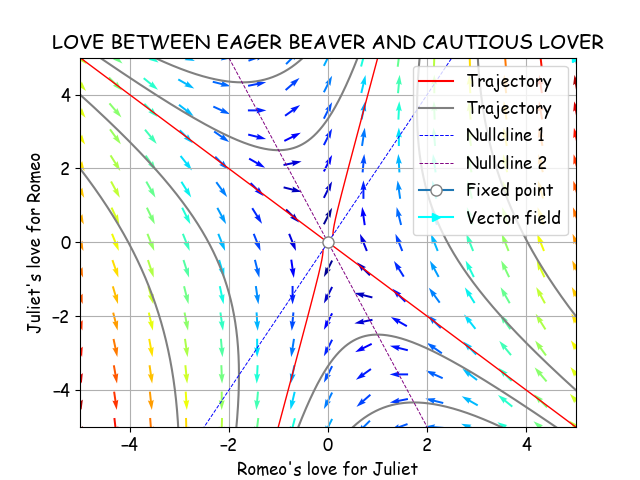
\includegraphics[width=100mm]{image/bt2/pp6.2.png}
    \caption{VD6.2 - The phase portrait of the love between Eager Beaver and Cautious Lover}
\end{figure}

\textbf{Dạng Phase portrait: } Saddle
\pagebreak
%%%%%%%%%%%%%%%%%%77777777777%%%%%%%%%%%%%%%%%%%%%%%%
%%%%%%%%%%%%%%%%%%%%%%%%%%%%%%%%%%%%%%%%%%%%%%%%%%%%%
\begin{tcbdoublebox}[title={7. Eager Beaver and Hermit}]
\mdseries .\\
\bfseries Ví dụ 1: \\
\textcolor{blue}{$$\left\{\begin{matrix}
\dot{R} =  5R +10J \\ 
\dot{J} =  -5R-5J\\ 
R(0)= -\frac{7}{2}, J(0)=\frac{3}{2}
\end{matrix}\right.$$}\\
\mdseries Ma trận $\color{blue}A=\begin{pmatrix}
5 & 10\\ 
-5 & -5
\end{pmatrix}$ có hai trị riêng là 
$\color{blue}\lambda_{1}=5i;\ \lambda_{2}=-5i$
, lần lượt tương ứng với các vecto riêng:
$\color{blue}v_{1} = (-1-i;\ 1)^{T};\ v_{2}=(-1+i;\ 1)^{T}$\\Áp dụng công thức bài tập 1, nghiệm của hệ phương trình là:
$$R(t)=-\frac{7\,\cos\left(5\,t\right)}{2}-\frac{\sin\left(5\,t\right)}{2}$$
$$J(t)=\frac{3\,\cos\left(5\,t\right)}{2}+2\,\sin\left(5\,t\right)$$
\\
\bfseries Ví dụ 2:\\
\textcolor{blue}{$$\left\{\begin{matrix}
\dot{R} = -3R -2J \\ 
\dot{J} =  4R +J\\ 
R(0)= -\frac{12}{5}, J(0)=\frac{9}{4}
\end{matrix}\right.$$}
\mdseries Ma trận $\color{blue}A=\begin{pmatrix}
-3 & -2\\ 
4 & 1
\end{pmatrix}$ có hai trị riêng là 
$\color{blue}\lambda_{1}=-1+2i;\ \lambda_{2}=-1-2i$
, lần lượt tương ứng với các vecto riêng:
$\color{blue}v_{1} = (-1+i;\ 2)^{T};\ v_{2}=(-1-i;\ 2)^{T}$\\Áp dụng công thức bài tập 1, nghiệm của hệ phương trình là:
$$R(t)=\frac{3\,\sin\left(2\,t\right)\,{\mathrm{e}}^{-t}}{20}-\frac{12\,\cos\left(2\,t\right)\,{\mathrm{e}}^{-t}}{5}$$
$$J(t)=\frac{9\,\cos\left(2\,t\right)\,{\mathrm{e}}^{-t}}{4}-\frac{51\,\sin\left(2\,t\right)\,{\mathrm{e}}^{-t}}{20}$$

\end{tcbdoublebox}
\pagebreak
\begin{figure}[!htbp]
    \centering
    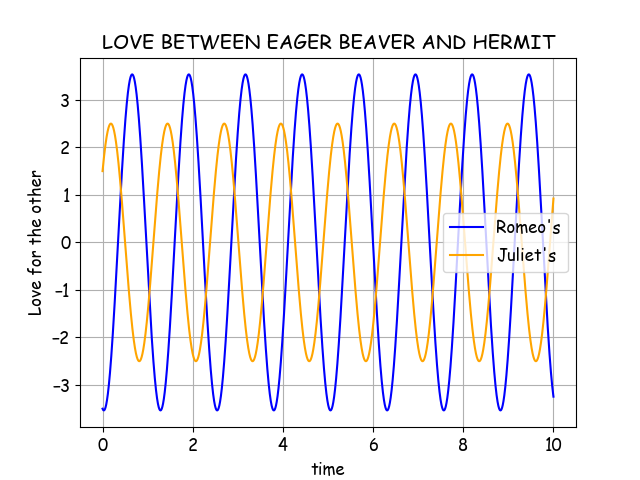
\includegraphics[width=100mm]{image/bt2/plot7.1.png}
    \caption{VD7.1 - The plot of the love between Eager Beaver and Hermit}
\end{figure}
\begin{figure}[!htbp]
    \centering
    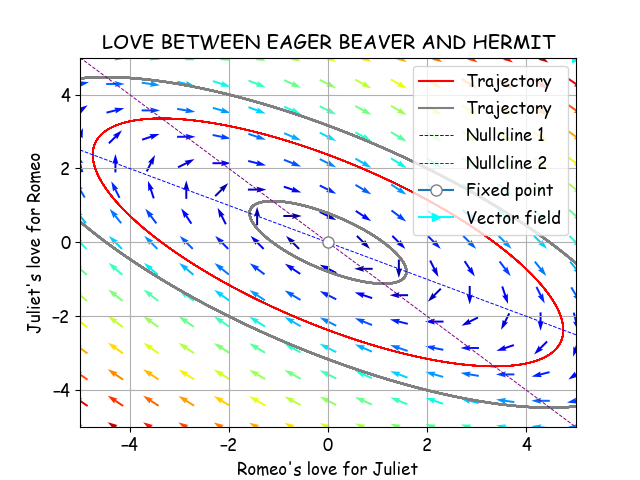
\includegraphics[width=100mm]{image/bt2/pp7.1.png}
    \caption{VD7.1 - The phase portrait of the love between Eager Beaver and Hermit}
\end{figure}

\textbf{Dạng Phase portrait: } Center
\pagebreak
\begin{figure}[!htbp]
    \centering
    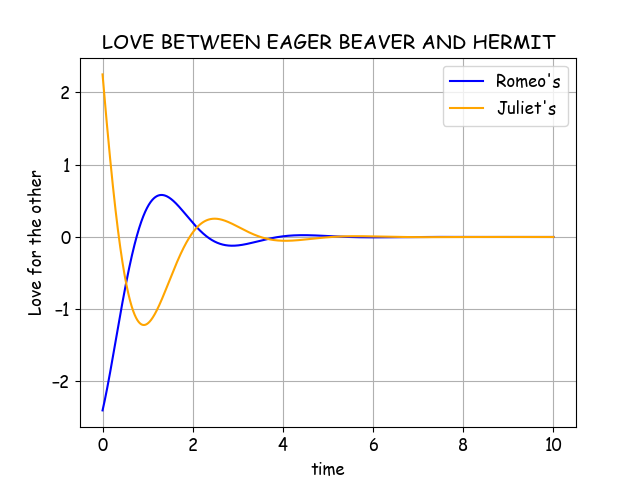
\includegraphics[width=100mm]{image/bt2/plot7.2.png}
    \caption{VD7.2 - The plot of the love between Eager Beaver and Hermit}
\end{figure}
\begin{figure}[!htbp]
    \centering
    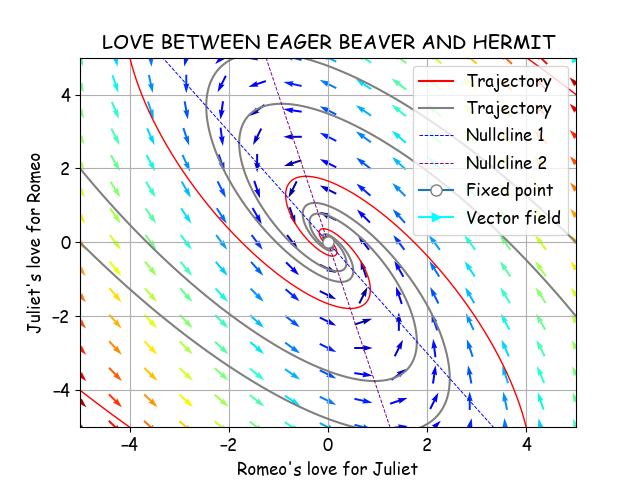
\includegraphics[width=100mm]{image/bt2/pp7.2.png}
    \caption{VD7.2 - The phase portrait of the love between Eager Beaver and Hermit}
\end{figure}

\textbf{Dạng Phase portrait: } Spiral Sink
\pagebreak
%%%%%%%%%%%%%%%%%%888888888888%%%%%%%%%%%%%%%%%%%%%%%%
%%%%%%%%%%%%%%%%%%%%%%%%%%%%%%%%%%%%%%%%%%%%%%%%%%%%%
\begin{tcbdoublebox}[title={8. Narcissistic Nerd and Cautious Lover}]
\mdseries .\\
\bfseries Ví dụ 1: \\
\textcolor{blue}{$$\left\{\begin{matrix}
\dot{R} =  2R -4J \\ 
\dot{J} =  R-2J\\ 
R(0)= -\frac{9}{2}, J(0)=3
\end{matrix}\right.$$}\\
\mdseries Ma trận $\color{blue}A=\begin{pmatrix}
2 & -4\\ 
1 & -2
\end{pmatrix}$ có trị riêng bội 2 là 
$\color{blue}\lambda_{1}=\lambda_{2}=0$ tương ứng với các vecto riêng:
$\color{blue}v = (2;\ 1)^{T};$\\Áp dụng công thức bài tập 1, nghiệm của hệ phương trình là:
$$R(t)=-21\,t-\frac{9}{2}$$
$$J(t)=3-\frac{21\,t}{2}$$
\\
\bfseries Ví dụ 2:\\
\textcolor{blue}{$$\left\{\begin{matrix}
\dot{R} = 3R -4J \\ 
\dot{J} =  5R -J\\ 
R(0)= -2, J(0)=-3
\end{matrix}\right.$$}
\mdseries Ma trận $\color{blue}A=\begin{pmatrix}
3 & -4\\ 
5 & -1
\end{pmatrix}$ có hai trị riêng là 
$\color{blue}\lambda_{1}=1+4i;\ \lambda_{2}=1-4i$
, lần lượt tương ứng với các vecto riêng:
$\color{blue}v_{1} = (2+4i;\ 5)^{T};\ v_{2}=(2-4i;\ 5)^{T}$\\Áp dụng công thức bài tập 1, nghiệm của hệ phương trình là:
$$R(t)=2\,\sin\left(4\,t\right)\,{\mathrm{e}}^t-2\,\cos\left(4\,t\right)\,{\mathrm{e}}^t$$
$$J(t)=-3\,\cos\left(4\,t\right)\,{\mathrm{e}}^t-\sin\left(4\,t\right)\,{\mathrm{e}}^t$$

\end{tcbdoublebox}
\pagebreak
\begin{figure}[!htbp]
    \centering
    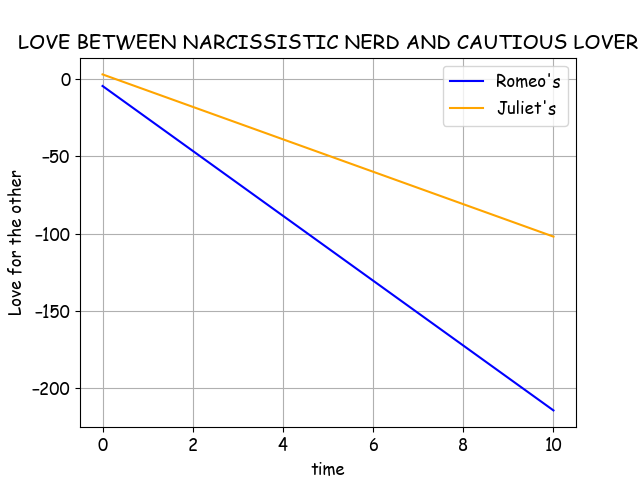
\includegraphics[width=100mm]{image/bt2/plot8.1.png}
    \caption{VD8.1 - The plot of the love between Narcissistic Nerd and Cautious Lover}
\end{figure}
\begin{figure}[!htbp]
    \centering
    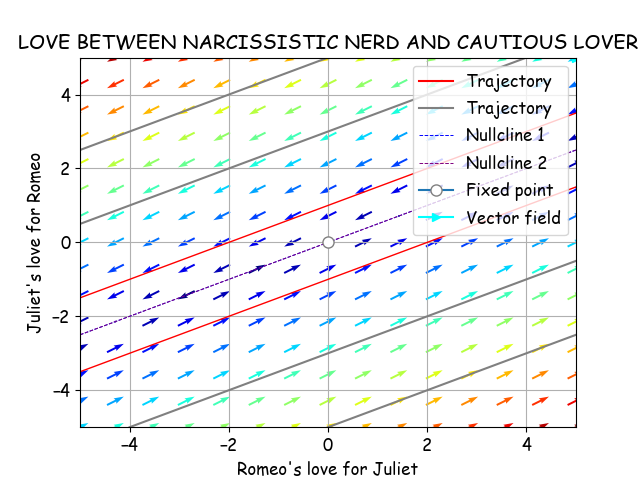
\includegraphics[width=100mm]{image/bt2/pp8.1.png}
    \caption{VD8.1 - The phase portrait of the love between Narcissistic Nerd and Cautious Lover}
\end{figure}

\textbf{Dạng Phase portrait: } Pure Shear
\pagebreak
\begin{figure}[!htbp]
    \centering
    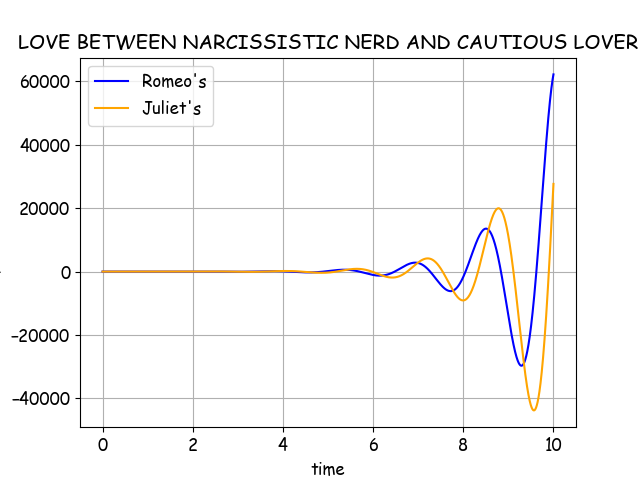
\includegraphics[width=100mm]{image/bt2/plot8.2.png}
    \caption{VD8.2 - The plot of the love between Narcissistic Nerd and Cautious Lover}
\end{figure}
\begin{figure}[!htbp]
    \centering
    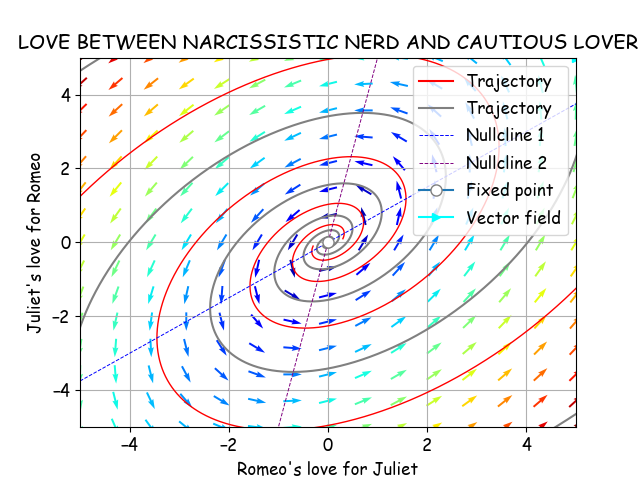
\includegraphics[width=100mm]{image/bt2/pp8.2.png}
    \caption{VD8.2 - The phase portrait of the love between Narcissistic Nerd and Cautious Lover}
\end{figure}

\textbf{Dạng Phase portrait: } Spiral Source
\pagebreak
%%%%%%%%%%%%%%%%%%99999999999%%%%%%%%%%%%%%%%%%%%%%%%
%%%%%%%%%%%%%%%%%%%%%%%%%%%%%%%%%%%%%%%%%%%%%%%%%%%%%
\begin{tcbdoublebox}[title={9. Narcissistic Nerd and Hermit}]
\mdseries .\\
\bfseries Ví dụ 1: \\
\textcolor{blue}{$$\left\{\begin{matrix}
\dot{R} =  3R -2J \\ 
\dot{J} =  -3R-2J\\ 
R(0)= 4, J(0)=4
\end{matrix}\right.$$}\\
\mdseries Ma trận $\color{blue}A=\begin{pmatrix}
3 & -2\\ 
-3 & -2
\end{pmatrix}$ có hai trị riêng là 
$\color{blue}\lambda_{1}=4;\ \lambda_{2}=-3$
, lần lượt tương ứng với các vecto riêng:
$\color{blue}v_{1} = (-2;\ 1)^{T};\ v_{2}=(1;\ 3)^{T}$\\Áp dụng công thức bài tập 1, nghiệm của hệ phương trình là:
$$R(t)=\frac{12\,{\mathrm{e}}^{-3\,t}}{7}+\frac{16\,{\mathrm{e}}^{4\,t}}{7}$$
$$J(t)=\frac{36\,{\mathrm{e}}^{-3\,t}}{7}-\frac{8\,{\mathrm{e}}^{4\,t}}{7}$$
\\
\bfseries Ví dụ 2:\\
\textcolor{blue}{$$\left\{\begin{matrix}
\dot{R} = 2R -1J \\ 
\dot{J} =  -4R -2J\\ 
R(0)= -2, J(0)=1
\end{matrix}\right.$$}
\mdseries Ma trận $\color{blue}A=\begin{pmatrix}
2 & -1\\ 
-4 & -2
\end{pmatrix}$ có hai trị riêng là 
$\color{blue}\lambda_{1}=2\sqrt{2};\ \lambda_{2}=-2\sqrt{2}$
, lần lượt tương ứng với các vecto riêng:
$\color{blue}v_{1} = (-1-\sqrt{2};\ 2)^{T};\ v_{2}=(-1+\sqrt{2};\ 2)^{T}$\\Áp dụng công thức bài tập 1, nghiệm của hệ phương trình là:
$$R(t)=\frac{\sqrt{8}\,{\mathrm{e}}^{-\sqrt{8}\,t}\,\left(\frac{\sqrt{8}}{4}-\frac{1}{2}\right)\,\left(\sqrt{8}-6\right)}{16}-{\mathrm{e}}^{\sqrt{8}\,t}\,\left(\frac{\sqrt{8}}{4}+\frac{1}{2}\right)\,\left(\frac{3\,\sqrt{8}}{8}+\frac{1}{2}\right)$$
$$J(t)={\mathrm{e}}^{\sqrt{8}\,t}\,\left(\frac{3\,\sqrt{8}}{8}+\frac{1}{2}\right)+\frac{\sqrt{8}\,{\mathrm{e}}^{-\sqrt{8}\,t}\,\left(\sqrt{8}-6\right)}{16}$$

\end{tcbdoublebox}
\pagebreak
\begin{figure}[!htbp]
    \centering
    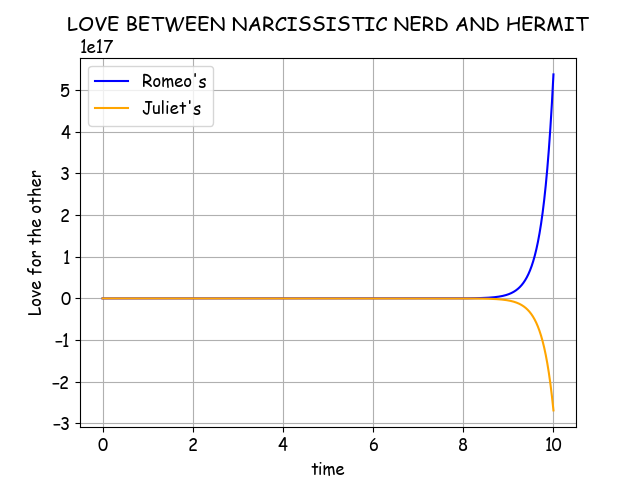
\includegraphics[width=100mm]{image/bt2/plot9.1.png}
    \caption{VD9.1 - The plot of the love between Narcissistic Nerd and Cautious Lover}
\end{figure}
\begin{figure}[!htbp]
    \centering
    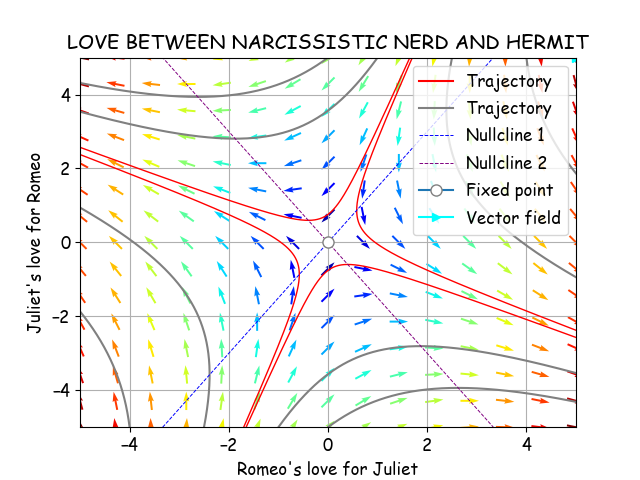
\includegraphics[width=100mm]{image/bt2/pp9.1.png}
    \caption{VD9.1 - The phase portrait of the love between Narcissistic Nerd and Hermit}
\end{figure}

\textbf{Dạng Phase portrait: } Saddle
\pagebreak
\begin{figure}[!htbp]
    \centering
    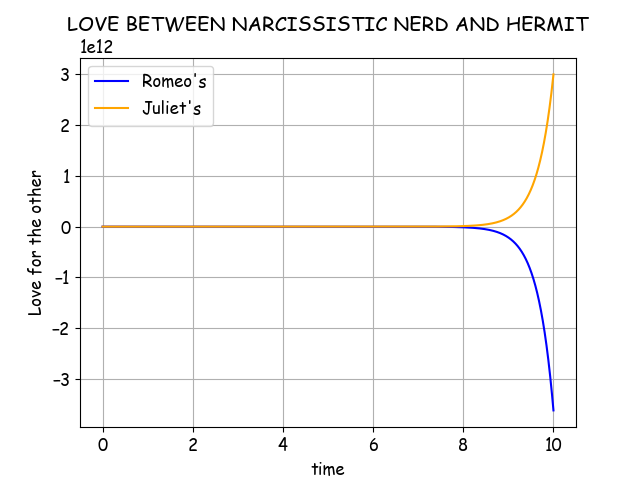
\includegraphics[width=100mm]{image/bt2/plot9.2.png}
    \caption{VD9.2 - The plot of the love between Narcissistic Nerd and Hermit}
\end{figure}
\begin{figure}[!htbp]
    \centering
    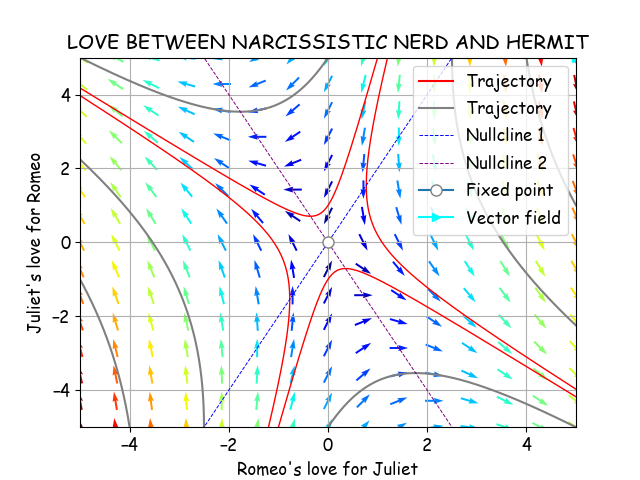
\includegraphics[width=100mm]{image/bt2/pp9.2.png}
    \caption{VD9.2 - The phase portrait of the love between Narcissistic Nerd and Cautious Lover}
\end{figure}

\textbf{Dạng Phase portrait: } Saddle
\pagebreak
%%%%%%%%%%%%%%%%%%101010101010%%%%%%%%%%%%%%%%%%%%%%%%
%%%%%%%%%%%%%%%%%%%%%%%%%%%%%%%%%%%%%%%%%%%%%%%%%%%%%
\begin{tcbdoublebox}[title={10. Cautious Lover and Hermit}]
\mdseries .\\
\bfseries Ví dụ 1: \\
\textcolor{blue}{$$\left\{\begin{matrix}
\dot{R} =  -2R +3J \\ 
\dot{J} =  -R-2J\\ 
R(0)= -\frac{12}{5}, J(0)=-\frac{9}{5}
\end{matrix}\right.$$}\\
\mdseries Ma trận $\color{blue}A=\begin{pmatrix}
-2 & 3\\ 
-1 & -2
\end{pmatrix}$ có hai trị riêng là 
$\color{blue}\lambda_{1}=-2+\sqrt{3}i;\ \lambda_{2}=-2-\sqrt{3}i$
, lần lượt tương ứng với các vecto riêng:
$\color{blue}v_{1} = (-\sqrt{3}i;\ 1)^{T};\ v_{2}=(\sqrt{3}i;\ 1)^{T}$\\Áp dụng công thức bài tập 1, nghiệm của hệ phương trình là:
$$R(t)=-\frac{12\,{\mathrm{e}}^{-2\,t}\,\cos\left(\sqrt{3}\,t\right)}{5}-\frac{9\,\sqrt{3}\,{\mathrm{e}}^{-2\,t}\,\sin\left(\sqrt{3}\,t\right)}{5}$$
$$J(t)=\frac{4\,\sqrt{3}\,{\mathrm{e}}^{-2\,t}\,\sin\left(\sqrt{3}\,t\right)}{5}-\frac{9\,{\mathrm{e}}^{-2\,t}\,\cos\left(\sqrt{3}\,t\right)}{5}$$
\\
\bfseries Ví dụ 2:\\
\textcolor{blue}{$$\left\{\begin{matrix}
\dot{R} = -6R -J \\ 
\dot{J} =  4R -2J\\ 
R(0)= -7, J(0)=4
\end{matrix}\right.$$}
\mdseries Ma trận $\color{blue}A=\begin{pmatrix}
-6 & -1\\ 
4 & -2
\end{pmatrix}$ có trị riêng bội hai là 
$\color{blue}\lambda_{1}=\lambda_{2}=-4$
, tương ứng với vecto riêng:
$\color{blue}v = (-1;\ 2)^{T}$\\Áp dụng công thức bài tập 1, nghiệm của hệ phương trình là:
$$R(0)=10\,t\,{\mathrm{e}}^{-4\,t}-7\,{\mathrm{e}}^{-4\,t}$$
$$J(t)=4\,{\mathrm{e}}^{-4\,t}-20\,t\,{\mathrm{e}}^{-4\,t}$$

\end{tcbdoublebox}
\pagebreak
\begin{figure}[!htbp]
    \centering
    \includegraphics[width=100mm]{image/bt2/plot10.1.png}
    \caption{V10.1 - The plot of the love between Cautious Lover and Hermit}
\end{figure}
\begin{figure}[!htbp]
    \centering
    \includegraphics[width=100mm]{image/bt2/pp10.1.png}
    \caption{VD10.1 - The phase portrait of the love between Cautious Lover and Hermit}
\end{figure}

\textbf{Dạng Phase portrait: } Spiral Sink
\pagebreak
\begin{figure}[!htbp]
    \centering
    \includegraphics[width=100mm]{image/bt2/plot10.2.png}
    \caption{VD10.2 - The plot of the love between Cautious Lover and Hermit}
\end{figure}
\begin{figure}[!htbp]
    \centering
    \includegraphics[width=100mm]{image/bt2/pp10.2.png}
    \caption{VD10.2 - The phase portrait of the love between Cautious Lover and Hermit}
\end{figure}

\textbf{Dạng Phase portrait: } Degenerate Nodal Sink
\pagebreak
\end{sol}
\pagebreak

\subsection{Bài tập 3}
\begin{problem}
   Let’s assume that the love between Romeo and Juliet is perturbed by outer
conditions, E.G. their families and social prejudices. In this case, the love is modeled by the IVP:
\textcolor{blue}{
\begin{align}\label{exercise-3-1}
    \begin{cases}
    \dot{R}=aR+bJ+f(t),\\
    \dot{J}=cR+dJ+g(t),\\
    R(0)=R_0,J(0)=J_0
    \end{cases}\tag{13}
\end{align}
}

Here $f$ and $g$ are two real functions dependent on $t$, e.g., $f(t) = t - 1$ and $g(t) = t^2$. Could we find the exact solution to the general \eqref{exercise-3-1}? If we could, give the formula of the solution and five
specific examples with their exact solutions. Otherwise, find general conditions on f and g so that the
\eqref{exercise-3-1} has a solution and also give five specific examples of such IVPs without finding the
exact solutions.  
\end{problem}

\begin{sol}
    Ta sẽ biến đổi hệ (13) về cấu trúc như sau: 
    \textcolor{blue}{\begin{align}\label{eq13-1}
        \begin{cases}
            \dot{X} = AX(t) + F(t), \\ 
            X(0) = X_0
        \end{cases}\tag{13.1}
    \end{align}}
    trong đó \textcolor{blue}{$$A=\begin{pmatrix}
   a &b\\
   c &d
\end{pmatrix},X(t)=\begin{pmatrix}
   R\\
   J
\end{pmatrix}, F(t)=\begin{pmatrix}
   f(t)\\
   g(t)\\
\end{pmatrix}, X_0 = \begin{pmatrix}
    R_0 \\
    J_0 \\
\end{pmatrix}$$}
Đây chính là \textit{\textcolor{blue}{hệ phương trinh vi phân cấp 1 tuyến tính không thuần nhất có giá trị ban đầu}}. Để giải quyết bài toán này, ta sử dụng một kỹ thuật gọi là \textit{\textbf{phương pháp biến thiên hằng số (Method of Variation of Constant)}} bao gồm các bước cụ thể sau: 

\begin{itemize}
 \item Ta sẽ tìm ma trận cơ bản \textcolor{blue}{$\Phi(t)$} từ nghiệm của hệ phương trình vi phân thuần nhất cấp 1 tương ứng \textcolor{blue}{$X(t) = AX(t), X(0) = X_0$. }
 \newline
 Gọi hai vector riêng trong công thức nghiệm tổng quát là \textcolor{blue}{$v_1 = \begin{pmatrix}
     \alpha_1 \\
     \alpha_2
 \end{pmatrix}$} và \textcolor{blue}{$v_2 = \begin{pmatrix}
     \alpha_3 \\
     \alpha_4
 \end{pmatrix}$}. Khi đó ma trận cơ bản của hệ phương rình vi phân tuyến tính thuần nhất cấp 1 biểu diễn là: 
 \textcolor{blue}{$$\Phi(t) = \begin{pmatrix}
     \alpha_1 e^{\lambda_1 t} & \alpha_2 e^{\lambda_2 t} \\
     \alpha_3 e^{\lambda_1 t} & \alpha_4 e^{\lambda_2 t} \\ 
 \end{pmatrix}$$}

 Vì \textcolor{blue}{$R, J$} là các hàm số phân biên nên $\Phi(t)$ có hai vector độc lập tuyến tính nên ma trận \textcolor{blue}{$\Phi(t)$} khả nghịch và có nghịch đảo là: 
 \textcolor{blue}{$$\Phi^{-1}(t) = \dfrac{1}{\det(\Phi(t))}\begin{pmatrix}
     \alpha_4 e^{\lambda_2 t} & -\alpha_3 e^{\lambda_2 t} \\
     -\alpha_2 e^{\lambda_1 t} & \alpha_1 e^{\lambda_1 t}
 \end{pmatrix}
 $$}

 \item Nghiệm  của hệ phương trình vi phân tuyến tính không thuần nhất \textcolor{blue}{\eqref{eq13-1}} được viết dưới dạng 
 \textcolor{blue}{$$X(t) = \Phi(t)C(t)$$}
 trong đó \textcolor{blue}{$C(t) = \begin{pmatrix}
     C_1(t) \\
     C_2(t) \\
 \end{pmatrix}$}. Thay ngược công thức nghiệm vào hệ \eqref{eq13-1} ta được: 
\textcolor{blue}{ $$X'(t)=AX(t)+F(t)
\newline
\Rightarrow \Phi'(t)C(t)+\Phi(t) C'(t)=A\Phi(t)C(t)+F(t)$$}
Chú ý rằng \textcolor{blue}{$\Phi(t)C(t)$} là nghiệm của hệ thuần nhất tương ứng nên \textcolor{blue}{$\Phi'(t)C(t) = A\Phi(t)C(t)$} nên rút gọn hai vế ta được: 
\textcolor{blue}{$$\Phi(t)C'(t)=F(t)$$}
Nhân \textcolor{blue}{$\Phi^{-1}(t)$} cho cả hai vế phương trình trên ta được: 
$$\textcolor{blue}{C'(t) = \Phi^{-1}F(t)}$$
Lấy tích phân cận từ $0$ tới $t$ thì ta được: 
\textcolor{blue}{$$ C(t)=C(0) +\int\limits_{0}^{t}\Phi^{-1}(s)F(s)ds$$}
Thay ngược lại vào công thức nghiệm thì ta được nghiệm của hệ \eqref{eq13-1} là: 
\textcolor{blue}{$$ X(t) = \Phi(t)C(0)+\Phi(t)\int\limits_{0}^{t} \Phi^{-1}(s)F(s)ds .$$}
thay $t = 0$ thì ta được 
\textcolor{blue}{$$X_0 = X(0) = \Phi(0)C(0) \Rightarrow C(0) = \Phi^{-1}(0)X_0 $$}
Từ đây, ta có nghiệm tổng quát của hệ phương trình \eqref{exercise-3-1} sẽ là: 
\textcolor{blue}{$$ X(t) = [\Phi(t)][\Phi^{-1}(0)]X_0+[\Phi(t)]\int\limits_{0}^{t} \Phi^{-1}(s)F(s)ds .$$}
\end{itemize}
\hspace{1cm}Vậy để nghiệm tồn tại thì tích phân phải có nghĩa, hay nói cách khác \textcolor{blue}{$\Phi^{-1}(t)F(t)$} tồn tại tích phân và các tích phân đó phả biểu diễn được ở dạng hàm sơ cấp để ta có thể biểu diễn nghiệm của hệ không thuần nhất một cách tường minh. Mặt khác, các hàm \textcolor{blue}{$f(t), g(t)$} phải liên tục.

\hspace{1cm }Hơn nữa, ở một số trường hợp đặc biệt hơn nếu \textcolor{blue}{$f(t), g(t)$} là các \textbf{\textit{giả đa thức (Quasi-polynominal)}}, thì khi đó ta có thể áp dụng \textbf{\textit{phương pháp hệ số bất định (Method of Undetermined Coefficients)}} để tìm nghiệm một cách dễ dàng hơn. 

\hspace{1cm} Khi đó \textcolor{blue}{$F(t) = \begin{pmatrix}
    f(t) \\
    g(t)
\end{pmatrix}$} được gọi là vector giả đa thức, tức là \textcolor{blue}{$F(t)$} có thể viết dưới dạng: 
\textcolor{blue}{$$ F(t) = e^{\alpha t} [\cos{(\beta t)}P_m(t) + \sin{(\beta t)} Q_n(t)]$$}
trong đó \textcolor{blue}{$\alpha, \beta$} là các số thực, \textcolor{blue}{$P_m(t), Q_n(t)$} lần lượt là các vector đa thức bậc m và n. Ví dụ, một vector đa \textcolor{blue}{$P_m(t)$} được viết dưới dạng: 
\textcolor{blue}{$$P_m(t) = A_0 + A_1 t + A_2 t^{2}+ ... + A_m t^{m} $$}
trong đó \textcolor{blue}{$A_0, A_1, A_2,..., A_m$} là các vector hệ số 2 chiều. 

\hspace{1cm} Trong trường hợp \textcolor{blue}{$f(t), g(t)$} là các \textit{giả đa thức}, thì nghiệm của hệ \textcolor{blue}{\eqref{exercise-3-1}} cũng là một vector giả đa thức, có cấu trúc tương tự với \textcolor{blue}{F(t)}, cụ thể nghiệm sẽ có dạng: 
\textcolor{blue}{$$X(t) = x^{s}e^{\alpha t}[\cos{(\beta t)} H_k(t) + \sin{(\beta t)} Q_k(t)]$$} 
trong đó \textcolor{blue}{$H_k(t), Q_k(t)$} là các đa thức bậc \textcolor{blue}{$k = max(m, n)$}. 
\end{sol} 
Bây giờ, ta xem xét các ví dụ sau:

\begin{example}
    Giải hệ phương trình: 
    $\textcolor{blue}{
    \begin{cases}
    \dot{R}=4R - 3J + e^{-t}\\
    \dot{J}=2R - J \\
    R(0)=4,J(0)=\dfrac{10}{3}
    \end{cases}
    }$
\end{example}
\begin{proof}
Hệ thuần nhất tương ứng là: \textcolor{blue}{$
    \begin{cases}
    \dot{R}=4R - 3J \\
    \dot{J}=2R - J \\
    \end{cases}
    $}
Phương trình đặc trưng của hệ thuần nhất: 
    $\begin{vmatrix}
4 - \lambda & -3 \\
2 & -1 - \lambda
\end{vmatrix} = 0 \Leftrightarrow \lambda^{2} - 3\lambda + 2 = 0 \Leftrightarrow \lambda = 1, \lambda = 2.\\$
Ứng với $\lambda = 1, \lambda = 2$, ta có hai vector riêng tương ứng là $P_1 = \begin{pmatrix}
    1 \\
    1
\end{pmatrix}$ và $P_2 = \begin{pmatrix}
    3 \\ 
    2
\end{pmatrix}$.
Ma trận nghiệm cơ bản của hệ thuần nhất:
$$\Phi(t) = \begin{pmatrix}
      e^{t} & 3e^{2t} \\
      e^{t} & 2e^{2t} \\ 
 \end{pmatrix}$$
Trong bài toán này ta thấy $f(t) = e^{-t}, g(t) = 0$ đều có tích phân tính biểu diễn được theo hàm sơ cấp, nên theo công thức nghiệm ở trên, nghiệm tổng quát của hệ là: 
$$ X(t) = [\Phi(t)][\Phi^{-1}(0)]X_0+[\Phi(t)]\int\limits_{0}^{t} \Phi^{-1}(s)F(s)ds 
$$
 $$= \begin{pmatrix}
      e^{t} & 3e^{3t} \\
      e^{t} & 2e^{2t} \\ 
 \end{pmatrix}.  \left[ \begin{pmatrix}
     1  & 3  \\
     1  & 2  \\ 
 \end{pmatrix}^{-1}.\begin{pmatrix}
     4 \\
    \dfrac{10}{3}  \\ 
 \end{pmatrix} +  \int\limits_{0}^{t} \begin{pmatrix}
     e^{s} & 3e^{3s} \\
     e^{s} & 2e^{2s} \\ 
 \end{pmatrix}^{-1}\begin{pmatrix}
     e^{-t}  \\
    0 \\ 
 \end{pmatrix}ds \right] $$
 $$
 = \begin{pmatrix}
     C_1 e^{t} & 3C_2e^{2t}  \\
     C_1 e^{t} & 2C_2 e^{2t} + \dfrac{1}{3} e^{-t} \\ 
 \end{pmatrix}.
 $$
 Thay t = 0, ta tìm được $C_1 = C_2 = 1$.
 \newline
 Vậy nghiệm của hệ là:$\begin{cases}
    R(t) =   e^{t} +  3e^{2t} \\
    J(t) =  e^{t} +  2 e^{2t} + \dfrac{1}{3} e^{-t} \\
    \end{cases} $
\end{proof}

\begin{example}
    Giải hệ phương trình: 
    $\textcolor{blue}{
    \begin{cases}
    \dot{R}=-3R + J + 3t\\
    \dot{J}=2R - 4J  + e^{-t}\\
    R(0)=4,J(0)= 7
    \end{cases}
    }$
\end{example}
\begin{proof}
    Hệ thuần nhất tương ứng là $\begin{cases}
    \dot{R}=-3R + J \\
    \dot{J}=2R - 4J \\
    \end{cases}$. Phương trình đặc trừng của hệ thuần nhất: $\begin{vmatrix}
-3 - \lambda & 1 \\
2 & -4 - \lambda
\end{vmatrix} = 0 \Leftrightarrow \lambda^{2} + 7\lambda + 10 = 0 \Leftrightarrow \lambda = -2, \lambda = -5.\\$
    Ứng với $\lambda = -2, \lambda = -5$, ta có hai vector riêng tương ứng là $P_1 = \begin{pmatrix}
    1 \\
    1
\end{pmatrix}$ và $P_2 = \begin{pmatrix}
    1 \\ 
    -2
\end{pmatrix}$.
Ma trận nghiệm cơ bản của hệ thuần nhất:
$$\Phi(t) = \begin{pmatrix}
     C_1 e^{-2t} & C_2 e^{-5t} \\
     C_1 e^{-2t} & -2C_2 e^{-5t} \\ 
 \end{pmatrix}$$

 Theo phương pháp biến thiên hằng số, nghiệm của phương trình (2) sẽ có dạng:
 $$\Phi(t) = \begin{pmatrix}
     C_1(t) e^{-2t} & C_2(t) e^{-5t} \\
  C_1(t) e^{-2t} & -2C_2(t) e^{-5t} \\    
 \end{pmatrix}$$
 hay
 $$\begin{cases}
     R(t) = C_1(t) e^{t} + C_2(t) e^{-5t} \\
    J(t) = C_1(t) e^{t} - 2C_2(t) e^{-5t} \\    
    \end{cases} $$
    Theo như chứng minh, thay lại vào hệ ban đầu thì ta được: 
    $$\Phi(t)C'(t)=F(t)$$
    $$\Rightarrow \begin{cases}
        C_1'(t)e^{-2t} + C_2'(t) e^{-5t} = 3t\\
        C_1'(t)e^{-2t} - 2C_2'(t)e^{-5t} = e^{-t}
    \end{cases}$$
    Giải hệ trên ta được 
    $$ \begin{cases}
        C_1'(t) = e^{2t}2t+\dfrac{e^{t}}{3}\\
        C_2'(t) = e^{5t}t-\dfrac{e^{4t}}{3} \\ 
    \end{cases}\Rightarrow\begin{cases}
        C_1(t) = e^{2t}t+\dfrac{e^{t}}{3} - \dfrac{e^{2t}}{2} + C_1\\
        C_2(t) = \dfrac{1}{5}e^{5t}t-\dfrac{e^{4t}}{12} - \dfrac{e^{5t}}{25}  + C_2\\ 
    \end{cases}$$

Với $t = 0$, ta có $\begin{cases}
    R(0) = C_1(0) + C_2(0) = 4 \\
    J(0) = C_1(0) - 2C_2(0) = 7 \\
\end{cases}$. Giải tìm được $C_1(0) = 5, C_2(0) = -1$, suy ra $C_1 = \dfrac{31}{6}, C_2 = -\dfrac{263}{300}$.
\end{proof}
\begin{example}
    Giải hệ phương trình: 
   $\textcolor{blue}{
    \begin{cases}
    \dot{R}= J + \dfrac{1}{\cos{t}}\\
    \dot{J}= - R\\
    R(0)=1,J(0)= 1
    \end{cases}
    }$ 
\end{example}
\begin{proof}
    Hệ thuần nhất tương ứng là: $
    \begin{cases}
    \dot{R}=J \\
    \dot{J}=-R \\
    \end{cases}
    $.
Phương trình đặc trưng của hệ thuần nhất: 
    $\begin{vmatrix}
 - \lambda & 1 \\
-1 &  - \lambda
\end{vmatrix} = 0 \Leftrightarrow \lambda^{2} + 1 = 0 \Leftrightarrow \lambda = i, \lambda = -i.\\$
Ứng với $\lambda = i, \lambda = -i$, ta có hai vector riêng tương ứng là $P_1 = \begin{pmatrix}
    \cos{t} \\
    -\sin{t}
\end{pmatrix}$ và $P_2 = \begin{pmatrix}
    \sin{t} \\ 
    \cos{t}
\end{pmatrix}$.
Vậy nghiệm cơ bản của hệ thuần nhất là 
$$\begin{cases}
    R(t) =  C_1\cos{t} +  C_2\sin{t} \\
    J(t) =  -C_1\sin{t} +  C_2\cos{t}\\
    \end{cases} $$
Áp dụng phương pháp biến thiên hằng số, công thức nghiệm của hệ không thuần nhất đề bài đưa ra là: 
$$\begin{cases}
    R(t) =  C_1(t)\cos{t} +  C_2(t)\sin{t} \\
    J(t) =  -C_1(t)\sin{t} +  C_2(t)\cos{t}\\
    \end{cases} $$
 Thế lại vào hệ không thuần nhất của đề bài và rút gọn ta được: 
 $$\begin{cases}
    C_1'(t)\cos{t} +  C_2'(t)\sin{t} = \dfrac{1}{\cos{t}} \\
   -C_1'(t)\sin{t} +  C_2'(t)\cos{t} = 0\\
    \end{cases} $$
 Giaỉ hệ trên ta tìm được $\begin{cases}
     C_1'(t) = 1\\
     C_2'(t) = \tan t
 \end{cases}\Rightarrow \begin{cases}
     C_1(t) = t + C_1\\
     C_2(t) = \ln{\vert\cos{t} \vert} + C_2
 \end{cases}$.
 \newline
 Từ đó thay vào ta được :$$\begin{cases}
    R(t) =  (t + C_1)\cos{t} +  (\ln{\vert\cos{t} \vert} + C_2)\sin{t} \\
    J(t) =  -(t + C_1)\sin{t} +  (\ln{\vert\cos{t} \vert} + C_2)\cos{t} \\
    \end{cases} $$
    
Với $R(0) = 1, J(0) = 1$, thay $t = 0$ ta có hệ:
$$\begin{cases}
    C_1 = 1\\
    1 + C_2 = 1
\end{cases} \Rightarrow \begin{cases}
    C_1 = 1\\
    C_2 = 0
\end{cases}$$
Vậy nghiệm của hệ là: 
$\begin{cases}
    R(t) =  (t + 1)\cos{t} +  \ln{\vert\cos{t} \vert}\sin{t} \\
    J(t) =  -(t + 1)\sin{t} +  \ln{\vert\cos{t} \vert}\cos{t} \\
    \end{cases} $
\end{proof}

\begin{example}
    Giải hệ phương trình: $\textcolor{blue}{
    \begin{cases}
    \dot{R}= 2R + 4J + \cos{t}\\
    \dot{J}=-R - 2J  + \sin{t}\\
    R(0)=1,J(0)= 3
    \end{cases}
    }$.
\end{example}
\begin{proof}
    Xét hệ phương trình thuần nhất tương ứng: 
    $$\begin{cases}
    \dot{R}= 2R + 4J\\
    \dot{J}=-R - 2J
    \end{cases}$$
    Phương trình đặc trưng của hệ thuần nhất: 
    $$\begin{vmatrix}
2 - \lambda & 4 \\
-1 &  -2 - \lambda
\end{vmatrix} = 0 \Leftrightarrow \lambda^{2}  = 0 \Leftrightarrow \lambda = 0.\\$$
Với $\lambda = 0$, ta tìm được vector riêng tương ứng là $\begin{pmatrix}
    2 \\
    -1
\end{pmatrix}$. Nghiệm sinh ra từ vector này là $\begin{cases}
    R = 2\\
    J = -1
\end{cases}$. 

Nghiệm thứ hai thêm biết $t$ vào nghiệm thứ nhất 
$$
\begin{pmatrix}
    R(t) \\
    J(t)
\end{pmatrix} = te^{0.t} \begin{pmatrix}
    2 \\
    -1
\end{pmatrix} + e^{0.t} \beta  
= t\begin{pmatrix}
    2 \\
    -1
\end{pmatrix} + \beta 
$$
với $\beta$ khác tạo ra nghiệm thỏa mãn được xác định thông qua phương trình:
$\begin{pmatrix}
    2 - \lambda & 4\\
    -1 & 2 -\lambda
\end{pmatrix} \beta = \begin{pmatrix}
    2 \\
    -1
\end{pmatrix}$ với $\lambda = 0$. Giải ra ta được $\beta = \begin{pmatrix}
    1 \\
    0
\end{pmatrix}$. Kết hợp hai nghiệm ta được nghiệm tổng quát của hệ thuần nhất: 
$$
\begin{cases}
    R(t) = 2C_1 + C_2(2t+1) \\
    J(t) = -C_1 - C_2 t
\end{cases}$$
Theo phương pháp biến thiên hằng số, nghiệm riêng của hệ không thuần nhất đề bài có dạng: 
$$
\begin{cases}
    R(t) = 2C_1(t) + C_2(t)(2t+1)\\
    J(t) = -C_1(t) - C_2(t)t
\end{cases}$$
Thay vào hệ không thuần nhất đề bài, rút gọn ta được: 
$$
\begin{cases}
    2C_1'(t) + C_2'(t)(2t+1) = \cos{t} \\
    -C_1'(t) - C_2'(t)t = \sin{t}
\end{cases}$$
Giải hệ ta được: 
$$
\begin{cases}
    C_1'(t) = -\sin{t} - t\cos{t} - 2t\sin{t} \\
    C_2'(t) = \cos{t} + 2\sin{t}
\end{cases} \Leftrightarrow \begin{cases}
    C_1(t) = -(t+2)\sin{t} + 2t\cos{t} + C_1 \\
    C_2(t) = \sin{t} - 2\cos{t} + C_2
\end{cases}
$$
Thay vào rút gọn ta được: 
$$\begin{cases}
    R(t) = -3\sin{t}-2\cos{t}+ C_2(2t+1)+2C_1 \\
    J(t) = 2\sin{t} - C_2t- C_1
\end{cases}$$
Thay t = 0, ta được 
$$\begin{cases}
    2C_1 + C_2 -2 = 1\\
    -C_1 = 3
\end{cases}$$
Giải hệ ta được 
$\begin{cases}
    C_1 = -3 \\
    C_2 = 9
\end{cases}$. Vậy nghiệm của hệ là:
$$\begin{cases}
    R(t) = -3\sin{t} - 2\cos{t} + 18t + 3 \\
    J(t) = 2\sin{t} - 9t + 3 
\end{cases}$$
\end{proof}

\begin{example}
Giải hệ phương trình: $\textcolor{blue}{\begin{cases}
    \dot{R} = -2R - 4J + (1 + 4t) \\
    \dot{J} = -R + J + \dfrac{3}{2} t^2 \\
    R(0) = 3, J(0) = 2
\end{cases}}$
\end{example}
\begin{proof}
    Xét hệ phương trình thuần nhất tương ứng: 
    $$\begin{cases}
    \dot{R}= -2R - 4J\\
    \dot{J}=-R + J
    \end{cases}$$
    Phương trình đặc trưng của hệ thuần nhất: 
    $$\begin{vmatrix}
-2 - \lambda & -4 \\
-1 &  1 - \lambda
\end{vmatrix} = 0 \Leftrightarrow \lambda^{2}  
 + \lambda - 6= 0 \Leftrightarrow \lambda = -3, \lambda = 2.\\$$
Ứng với hai vector riêng $\lambda_1 = -3, \lambda_2 = 2$ ta có lần lượt có hai vector riêng là $\begin{pmatrix}
    4 \\
    1
\end{pmatrix},  \begin{pmatrix}
    -1 \\
    1
\end{pmatrix}$.  Vậy nghiệm của hệ thuần nhất: 
$$
\begin{cases}
    R(t) = 4C_1e^{-3t} - C_2e^{2t} \\
    J(t) = C_1e^{-3t} + C_2e^{2t}
\end{cases}$$
Theo phương pháp biến thiên hằng số, nghiệm không thuần nhất của hệ sẽ có dạng: 
$$\begin{cases}
    R(t) = 4C_1(t)e^{-3t} - C_2(t)e^{2t} \\
    J(t) = C_1(t)e^{-3t} + C_2(t)e^{2t}
\end{cases}$$
Thay lại vào hệ không thuần nhất rút gọn ta được: 
$$\begin{cases}
    4C_1'(t)e^{-3t} - C_2'(t)e^{2t} = 1 + 4t \\
    C_1'(t)e^{-3t} + C_2'(t)e^{2t} = \dfrac{3}{2}t^2
\end{cases}$$
Giải hệ ta được: 
$$\begin{cases}
    C_1'(t) = e^{3t}\left[\dfrac{1}{5}(1+4t) + \dfrac{3}{10}t^2 \right]\\
    C_2'(t) = \dfrac{1}{5}e^{3t}(6t^2 - 4t - 1)
\end{cases} \Leftrightarrow \begin{cases}
    C_1(t) = \dfrac{te^{3t}(t+2)}{10} + C_1 \\
    C_2(t) = \dfrac{2}{5}t^2e^{3t}-\dfrac{8}{15}te^{3t}+\dfrac{1}{9}e^{3t} + C_2
\end{cases}$$
Từ công thức $R(t), J(t)$ thay t = 0, kết hợp $R(0), J(0)$ giải ra ta được $C_1(0) = 1, C_2(0) = 1$. Suy ra $C_1 = 1, C_2 = \dfrac{8}{9}$. Vậy nghiệm của hệ phương trình đè bài là: 
$$
\begin{cases}
    R(t) = 4C_1(t)e^{-3t} - C_2(t)e^{2t} \\
    J(t) = C_1(t)e^{-3t} + C_2(t)e^{2t}
\end{cases}$$
với 
$$\begin{cases}
    C_1(t) = \dfrac{te^{3t}(t+2)}{10} + 1 \\
    C_2(t) = \dfrac{2}{5}t^2e^{3t}-\dfrac{8}{15}te^{3t}+\dfrac{1}{9}e^{3t} + \dfrac{8}{9}
\end{cases}$$
\end{proof}
\begin{problem}
A more general and also complicated love between Romeo and Juliet is the IVP
\textcolor{blue}{
\begin{align}\label{exercise-3-2}
    \begin{cases}
    \dot{R}=f(t,R,J)\\
    \dot{J}=g(t,R,J)\\
    R(0)=R_0,J(0)=J_0
    \end{cases}\tag{14} 
\end{align}
}
where f and g are two real functions dependent on t, R, and J. Similarly, find conditions on $f$ and
$g$ so that the IVP Sys. (14) has a solution. For example, a solution exists for IVP Sys. (14) where
\textcolor{blue}{$f(R, J) = R(1 - J)$} and \textcolor{blue}{$g(R, J) = J(R - 1)$} (this is also known as the Lotka–Volterra equations in Biology to model the interaction of two species). Give five specific examples of such IVPs without
finding the exact solutions.
\end{problem}
\begin{proof}
    Trước khi bàn về điều kiện có nghiệm, đầu tiên ta tìm hiểu về định nghĩa sau: 
    \begin{definition}[Lipschizt Continunity]
        Một hàm số $f:X\to Y$ được gọi là thỏa \textbf{liên tục Lipschizt} nếu tồn tại hằng số dương $L$ thỏa mãn với mọi $(x_1, y),(x_2, y)\in X$ sao cho  
$$\left|f(x_1, y)-f(x_2, y)\right|\le L|x_1-x_2|$$
    \end{definition}
Ở đây không phải là định nghĩa tổng quát nhất về \textit{liên tục Lipschizt}, nhưng ta chỉ bàn về hàm số khả vi liên tục trên tập số thực nên định nghĩa ở trên là đủ để cho bài toán này.
\newline
Tiếp theo, ta sẽ phát biểu về một định lý về sự tồn tại và duy nhất đối với trường hợp tổng quát hệ phương trình \textit{\textcolor{blue}{IVPs Sys 14}}.
\begin{theorem}[Định lý Picard–Lindelöf]
Xét hệ gồm n phương trình vi phân cấp I có dạng \textit{chuẩn tắc} (dạng giải ra được đối với đạo hàm) nếu có thể viết dưới dạng: 
$$
\begin{cases}
    \dot{y_1} = f_1(x, y_1, y_2,..., y_n)\\
    \dot{y_2} = f_2(x, y_1, y_2,...,y_n)\\
    ... \\
    \dot{y_n} = f_n(x, y_1, y_2,..,y_n) \\
    y_i(x_0) = y_i^0, i = \overline{1,n}
\end{cases} or \begin{cases}
    \dot{y} = f(x,y) \\
    y(x_0) = f(x_0,y_1^0,...,y_n^0) \\
    y = (y_1, y_2,..., y_n)^T, f = (f_1, f_2,..., f_n)^T \\
\end{cases}$$
trong đó $x$ là biến độc lập, $f_i$ là các hàm khả vi liên tục trên $\mathbb{R} \times \mathbb{R}^n$ và $y_i$ là các ẩn hàm cần tìm.
\newline
Giả sử các hàm $f_1, f_2,..., f_n$ là liên tục trên một tập mở $G \subset \mathbb{R}^{n+1}$ chứa $(x_0, y_1^0,...,y_n^0)$ và \textit{liên tục Lipschizt} theo biến y.Khi đó tồn tại số thực $\varepsilon >0$ sao cho  có duy một nghiệm $y_1(x), y_2(x),..., y_n(x)$ thỏa với trên đoận $[t_0-\varepsilon,t_0+\varepsilon]$. 
\end{theorem}
Để chứng minh định lý trên cần kiến thức về không gian metric cũng như một số định lý và bổ đề như \textbf{Banach fixed-point theorem} nên ở đây chỉ xem xét về mặt ứng dụng của nó mà bỏ qua chứng minh định lý.
\newline
Quay trở lại bài toán, ta có thể đặt $y = (R,T)^T,  F = (f,g)^T$ thì bài toán chuyển thành:
$$
\begin{cases}
    \dot{y} = F(t,y) \\
    y(0) = (R_0, J_0)^T
\end{cases}
$$
Từ định lý trên ta thấy rằng nếu các hàm $f(t, R, J), g(t, R, J)$ liên tục trên tập mở $G \subset \mathbb{R}^3$ chứa \textit{giá trị ban đầu (\textbf{inital value})} và thỏa \textit{điều kiện Lipschizt} theo $y$ thì theo \textbf{định lý Picard-Lindelöf}, tồn tại số thực $\varepsilon > 0$ sao cho tồn tại nghiệm R(t), J(t) duy nhất nằm trong khoảng $[-\varepsilon, \varepsilon]$. Tuy vậy đây chỉ là \textit{nghiệm địa phương của hệ (local solution)} chứ ta vẫn chưa đảm bảo được đây là nghiệm trên toàn tập xác định. 
\newline
\newline
Ta sẽ bàn tiếp về vấn đề gọi là thác triển nghiệm toàn cục. Để giải quyết vấn đề này ta bàn đến chủ đề khoảng tồn tại của nghiệm, cụ thể ở đây là về vấn đề \textit{khoảng tồn tại cực đại} của nghiệm (\textbf{Maximal Interval Existence}) khi các giả thiết trong \textbf{định lý Picard-Lindelöf} được thỏa mãn. Ta sẽ bắt đầu với một số định nghĩa quan trọng và một định lý liên quan tới mảng  \textit{giải tích thực (real analysis)}.
\begin{definition}
    Cho hàm số $ f: \mathcal{D} \subseteq \mathbb{R} \times \mathbb{R}^n \rightarrow \mathbb{R}^n $. Ta nói $f(t,x)$ là \textit{liên tục Lipschizt} địa phương với biến $x$ trên $\mathcal{D}$ nếu với mỗi $(t_0, a) \in \mathcal{D}$ tồn tại số thực dương $L$ và một tập $\mathcal{I} \times \mathcal{U} \subseteq \mathcal{D}$ chứa $(t_0, a)$ trong miền của nó và $f(t,x)$ lên tục Lipschizt đối với miền $\mathcal{U}$ với hằng số Lipschizt là $L$ với mọi $t \in \mathcal{I}$.
\end{definition}

\begin{theorem}[Maximal Interval of Existence]
    Hệ phương trình \textit{\textcolor{blue}{IVP Sys 14}} có một khoảng tồn tại cực đại, có dạng $(\omega_-, \omega_+)$, với $\omega_- \in [-\infty; +\infty), \omega_+ \in (-\infty; +\infty]$. Tồn tại một nghiệm duy nhất R(t), J(t) của \textit{\textcolor{blue}{IVP Sys 14}} trên $(\omega_-; \omega_+)$ và $(t, R(t), J(t))$ luôn có thể nằm ngoài một tập con $\mathcal{K}$ của $\mathcal{D}$ khi t tiến về $\omega_-$ và t tiến về $\omega_+$.
\end{theorem}
Định lý này được trích trong trang 15 cuốn \textit{Theory of Ordinary Differential Equations} của \textit{Christopher P.Grant, Brigham Young University}.

Từ định lý trên, ta có hai hệ quả như sau: 
\begin{corollary}
    Nếu $\mathcal{D}'$ là một tập hợp bị chặn và $\mathcal{D} = (c,d) \times \mathcal{D}'$ (với $c \in [-\infty; +\infty)$ và $d \in (-\infty; +\infty]$) thì $\omega_+ = d$ hoặc $y(t) \rightarrow \partial\mathcal{D}'$ khi $t$ tiến về $\omega_+$ và $\omega_- = c$ hoặc $y(t) \rightarrow \partial\mathcal{D}'$ khi $t$ tiến về $\omega_-$.
\end{corollary}
\begin{corollary}
    Nếu $\mathcal{D} = (c,d) \times \mathbb{R}^n$ (với $c \in [-\infty; +\infty)$ và $d \in (-\infty; +\infty] $), khi đó $\omega_+ = d$ hoặc $\vert y(t) \vert \rightarrow \infty$ khi $t$ tiến về $\omega_+$ và $\omega_- = c$ hoặc $\vert y(t) \vert \rightarrow \infty$ khi $t$ tiến về $\omega_-$
\end{corollary}
Từ hệ quả thứ hai ta thấy rằng, mọi hệ được tổng quát từ \textcolor{blue}{\textit{IVP Sys 14}} nói chung và bản thân \textcolor{blue}{\textit{IVP Sys 14}} nói riêng trên tập $ \mathbb{R}^n$ có nghiệm thác triển tồn tại trên toàn tập xác định $t \in \mathbb{R}$ \textit{(unbounded)}.
\newline
Ta chú ý rằng khoảng tồn tại cực đại: 
\begin{itemize}
    \item Có thể là tập con của R.
    \item Tùy thuộc vào giá trị ban đầu \textit{(initial value)}.
\end{itemize}
Bây giờ, ta sẽ xem xét qua một số ví dụ điển hình như sau: 
\begin{example}
    Giải hệ phương trình sau theo $x$ tập xác định $(0;+\infty)$: 
    $$\begin{cases}
        \dot{y_1} = y_2 \\
        \dot{y_2} = -\dfrac{1}{x}y_2 + \dfrac{1}{x^2}y_1
    \end{cases}$$
    Đây là dạng biến đổi của  \textbf{\textit{phương trình vi phân cấp 2 Cauchy-Euler}}. Ta có thể thay phương trình thứ nhất xuống phương trình thứ hai sẽ được: 
    $$
        y_1'' + xy_1' - y_1 = 0
    $$
    Theo \textbf{định lý 2.4.2} trong \textit{trang 120} quyển \textit{Ordinary Differential Equation} của \textit{Gabriel Nagy} thì phương trình có nghiệm 
    $$y_1 = c_1x^1 + c_2 x^{-1} = c_1x + \dfrac{c_2}{x}$$
    Vậy nghiệm của hệ là: 
    $$
    \begin{cases}
        y_1 = c_1x + \dfrac{c_2}{x} \\
        y_2 = c_1 - \dfrac{c_2}{x^2}
    \end{cases}
    $$
\end{example}

\begin{example}
    Đặt $u = (R, T)$, chuyển về dạng vector ta sẽ giải hệ sau theo biến t:
    $$\begin{cases}
        \dot{u} = Au^{\dfrac{2}{3}} \\
        u(0) = 0
    \end{cases}$$
    với A là vector hệ số.
\end{example}
\begin{proof}
    Ta thấy rằng hàm số $f(t, u) = Au^{\dfrac{2}{3}}$ liên tục nhưng không liên tục Lipschizt theo biến u trong lân cận bất kỳ của $(0,0)$ nên hệ trên không có nghiệm duy nhất. Thật vậy, ta dễ dàng thấy hai nghiệm thỏa mãn phương trình như sau: 
    $$ y(t) = 0$$
    hoặc 
    $$y(t) = \begin{cases}
        \left(\dfrac{Ax}{3} \right)^3 \hspace{0.5cm} (t \geq 0) \\
        0 \hspace{1.5cm} (t < 0)
    \end{cases}$$
    
\end{proof}

\begin{example}[Mô hình thú săn mồi - con mồi]
    Sự phát triển của hai quần thể sinh vật (chẳng hạn $x=x(t)$ là số con mèo và $y = y(t)$ là số con chuột) theo thời gian được mô tả bởi hệ phương trình Loktra-Volterra sau đây: 
    $$\begin{cases}
        y' = y(\alpha - \beta x) \\
        x' = x(\gamma y - \delta)
    \end{cases}$$
    với $\alpha, \beta, \gamma, \delta$ là những hằng số đặc trưng cho sự tăng trưởng toán học của quần thể.
\end{example}
Nghiệm của phương trình Loktra-Volterra được cho bởi: 
$$\gamma y - \delta \ln{y} = \alpha \ln{x} - \beta x + C$$

\begin{example}
    Xét hệ phương trình:
    $$
    \begin{cases}
        y' = \sqrt{ax^2 + by^2 + e} \\
        x' = \sqrt{cy^2 + dy^2 + f}
    \end{cases}$$
    Xét $f(t,x,y) = \sqrt{ax^2 + by^2 + e}$ có:
    $$
    \begin{tabular}{cl}
        $\vert f(t,x_1, y_1) - f(t, x_2, y_2) \vert$ & = $ \left| \dfrac{a(x_1^2 - x_2^2) + b(y_1^2 - y_2^2)}{\sqrt{ax_1^2 + by_1^2 + e} + \sqrt{ax_2^2 + by_2^2 + e}} \right|$ \\
    & $\leq \vert a \vert \dfrac{\vert x_1 - x_2 \vert \vert x_1 + x_2 \vert}{\sqrt{ax_1^2 + by_1^2 + e} + \sqrt{ax_2^2 + by_2^2 + e}} + \vert b \vert  \dfrac{\vert y_1 - y_2 \vert \vert y_1 + y_2 \vert}{\sqrt{ax_1^2 + by_1^2 + e} + \sqrt{ax_2^2 + by_2^2 + e}}$ \\
    & $\leq  \vert a \vert\vert x_1 - x_2 \vert + \vert b \vert \vert y_1 - y_2 \vert \leq M (\vert x_1 - x_2 \vert +  \vert y_1 - y_2 \vert)  $
    \end{tabular} $$
    với $M = \max (\vert a \vert,\vert b \vert)$. Vậy hàm $f(t,x, y)$ liên tục Lipschizt theo $(x,y)$. 
    \newline 
    Chứng minh tương tự $g(t,x,y) = \sqrt{cy^2 + dy^2 + f}$ cũng liên tục Lipschizt. Mặt khác $f(t,x,y)$ và $g(t,x,y)$ liên tục trên R nên theo định lý Picard-Lindelof thì hệ này có nghiệm.    
\end{example}

\begin{example}
    Cho hệ phương trình vi phân sau
$$
\begin{cases}
R'(t)=a\cos(R(t))+b\sin(J(t))\\
J'(t)=c\cos(R(t))+d\sin(J(t))
\end{cases}
$$
\end{example}
Ta có:
$$
\begin{array}{l}
R' = f( t,R,J) =  a\cos(R) \ +\ b\sin(J)\\
J' = g( t,R,J) = c\cos(R) \ +\ d\sin(J)
\end{array}
$$
  Xét hàm $g(t,R,J)$ : 
  \begin{center}
      \begin{tabular}{cl}
   $
|g( t,R_{1} ,J_{1}) -g( t,R_{2} ,J_{2}) |
$    & $
 = \left| \left( ccos( R_{1}) +dsin( J_{1}) \right) - \left( ccos( R_{2}) +dsin( J_{2}) \right) \right| $ \\
       & $
= |c( cos( R_{1}) -cos( R_{2})) +d( sin( J_{1}) -bsin( J_{2})) | $\\
& $\leqslant  |c( R_{1} -R_{2}) +d( J_{1} -J_{2}) |
$
  \end{tabular}
  \end{center}
  
Mặt khác: 
  $$|c(R_1-R_2)|+|d(J_1-J_2)|  \leqslant N  (|R_1-R_2| + |J_1-J_2|)$$
  với $N = \max (\vert a \vert, \vert b \vert).$
Suy ra: 
$$|g( t,R_{1} ,J_{1}) -g( t,R_{2} ,J_{2}) |\ \leqslant \ N  (|R_1-R_2| + |J_1-J_2|)$$ 
với $N = \max (\vert a \vert, \vert b \vert).$ Suy ra $g(t,R,J)$ liên tục Lipschizt theo $(x,y)$.
\newline
Chứng minh tương tự, ta cũng suy ra đc $f(t,R,J)$ cũng liên tục Lipschizt theo $(x,y)$. Từ đó, theo định lý Picard-Lindelof và đây là hệ có nghiệm.
\end{proof}
\subsection{Bài tập 4}
\begin{problem}
    This exercise shows us how to solve the IVPs Sys. (13) and Sys. (14) “numerically” when the existence of solutions is guaranteed. The most straightforward numerical scheme
is the explicit Euler method.
    This function receives the value $R_0$ and $J_0$ of $R(t)$ and $J(t)$ at time $t_0$ and returns the approximate values $R_1$ and $J_1$ at $t_1 = t_0 + h$, where $h$ is the time step. The "Local Truncation Error" at $t_1$ is thus define by 
    $$\mathcal{E}(t_1) := \sqrt{[R(t_1) - R_1]^2 + [J(t_1) - J_1]^2}$$ \\
    Prove that $\mathcal{E}(t_1)$ is proportional to $h^2$
\end{problem}
\begin{sol}
Trước khi đi vào giải quyết vấn đề, ta cần nhắc lại về \textbf{\textit{Định lý Taylor:}} \\
Trong giải tích, định lý Taylor cho ta một đa thức xấp xỉ một hàm khả vi tại một điểm cho trước (gọi là đa thức Taylor của hàm đó) có hệ số chỉ phụ thuộc vào các giá trị của đạo hàm tại điểm đó. Một phát biểu cơ bản của định lý Taylor là: 
Cho n là số nguyên dương và f là hàm khả vi liên tục đến cấp n trên khoảng đóng [a,x] và khả vi cấp n+1 trên khoảng mở (a,x) thì: \\
\begin{center}
    \begin{math}
    f(x) = f(a) + \dfrac{f'(a)}{1!}(x-a) + \dfrac{f^{(2)}(a)}{2!}(x-a)^{2} +...+ \dfrac{f^{(n)}(a)}{n!}(x-a)^{n} + R_{n}(x) 
\end{math} \\
\end{center}

Vì $R(t)$ và $J(t)$ là các hàm số khả vi vô hạn lần trên khoảng đóng $[t_0, t_1]$, áp dụng khai triển Taylor tới bậc 1 tại $t = t_0$ cho hai hàm số trên với phần dư Lagrange, tồn tại $a, b \in (t_0, t_1)$ thỏa: \\
$$ \begin{cases}
    R(t_1) = R(t_0) + R'(t_0)(t_1 - t_0) + \dfrac{R''(a)}{2!}(t_1 - t_0)^{2} \\ 
    J(t_1) = J(t_0) + J'(t_0)(t_1 - t_0) + \dfrac{J''(b)}{2!}(t_1 - t_0)^{2}
\end{cases}$$
Bên cạnh đó, ta có định nghĩa của hệ phương trình vi phân ban đầu: 
$$\begin{cases}
    R'(t) = f(t, R(t), J(t)) \\
    J'(t) = g(t, R(t), J(t))
\end{cases} $$

Từ hai hệ phương trình trên, kết hợp với điều kiện $t_1 - t_0 = h$, ta có: \\
$$\begin{cases}
    R(t_1) = R(t_0) + f(t_0, R(t_0), J(t_0)).h + \dfrac{R''(a)}{2!}h^{2} \\
    J(t_1) = J(t_0) + g(t_0, R(t_0), J(t_0)).h + \dfrac{J''(b)}{2!}h^2 
\end{cases} $$
Tương đương: 
$$\begin{cases}
    R(t_1) = R_1 + \dfrac{R''(a)}{2!}h^{2} \\
    J(t_1) = J_1 + \dfrac{J''(b)}{2!}h^{2}
\end{cases}$$
Quay lại định nghĩa về "local truncation error" được đề cập: 
\begin{equation} 
\begin{split}
\mathcal{E}(t_1) 
&     = \sqrt{[R(t_1) - R_1)]^{2} + [J(t_1) - J_1]^{2}} \\
&   = \sqrt{[\dfrac{R''(a)}{2!}h^{2}]^{2} + [\dfrac{J''(b)}{2!}h^{2}]^{2}} \\
&   = \sqrt{\dfrac{R''(a)^2}{4} + \dfrac{J''(b)^2}{4}} .h^{2}
\end{split}
\end{equation} \\

Đồng nghĩa với việc $\mathcal{E}(t_1)$ tỉ lệ với $h^{2}$

\end{sol}
\begin{problem}
    One of the advantages of this numerical scheme is the fast running time. However, this scheme is
not “stable” for large-time step $h$. For some problems, it requires $h<1$. In this case, we must consider
the “implicit” Euler method. 
\end{problem}
\begin{sol}
    \textbf{\textit{Phương pháp Explicit Euler}} là một phương pháp số bậc một để giải các phương trình vi phân thường (ODEs) với giá trị ban đầu cho trước (initial value). \\
    Đối với những phương trình vi phân phức tạp, việc tính toán gần đúng các giá trị có vai trò hết sức quan trọng. Để dễ hình dung, một cách phi chính thức, ta có thể đặt vấn đề xác định hình dạng của một đường cong thỏa mãn phương trình vi phân mà ta rất khó để tìm được lời giải.
    Phương pháp Explicit Euler lấy ý tưởng ta có thể tính toán được độ dốc của tiếp tuyến (hay giá trị đạo hàm) tại điểm bất kỳ trên đường cong một khi xác định được vị trí của điểm đó. Nhờ vậy ta có thể dự đoán được xu hướng tiếp theo của hình dạng của đường cong, và tính toán gần đúng giá trị tại điểm tiếp theo thông qua bước nhảy $h$. Như đã chứng minh ở trên, sai số cục bộ của mỗi bước nhảy tỉ lệ thuận với bình phương độ dài bước nhảy, chính vì vậy phương pháp Explicit Euler chỉ ổn định khi ta thực hiện tính toán với bước nhảy $h < 1$ (như đã được đề cập trong đề bài). \\
    Giả sử ta có bài toán: 
\begin{center}
    $\begin{cases}
        Y'(t) = F(Y(t), t) \\
        Y(t_0) = Y_0
\end{cases} $
\end{center}
    Bài toán như trên được gọi là bài toán Cauchy, với giá trị cho $Y_0$ được cho trước tại $t = t_0$. Như đã đề cập, đối với hàm $F(Y(t), t)$ đơn giản, ta có thể dễ dàng tìm ra được lời giải. Tuy nhiên với hàm số $F(Y(t), t)$ bất kì thì chúng ta không có phương pháp giải tổng quát, hay nói cách khác việc có thể tìm ra được lời giải phụ thuộc vào dạng của hàm $F(Y(t),t)$. Chính vì vậy, một cách tiếp cận thuần số học là ta có thể sử dụng liên tục các bước nhảy để đi tìm giá trị của hàm số tại một điểm bất kì từ giá trị cho trước. Cụ thể, ta có thể tính xấp xỉ giá trị của Y(t) bằng dãy $Y(t_n)$ thỏa: \\
   \begin{center}
        $\begin{cases}
        Y(t_0) = Y_0 \\
        Y(t_{n+1}) = Y(t_n) + h.F(Y(t_n), t_n)
    \end{cases} $
   \end{center}
    Với bước nhảy $h = t_{n+1} - t_n$ và $F(Y(t_n), t_n)$ chính là độ dốc của tiếp tuyến tại $t = t_n$ \\ 
    Đối với bước nhảy h lớn, phương pháp Implicit Euler thường được sử dụng hơn vì những phương pháp Implicit không bị ràng buộc bởi độ dài của bước nhảy. Để hiểu rõ hơn, phương pháp Implicit Euler gần như tương tự Explicit Euler, chỉ khác ở chỗ giá trị xấp xỉ của Y(t) được tính bằng dãy $Y(t_n)$ thỏa: 
    \begin{center}
        $\begin{cases}
        Y(t_0) = Y_0 \\
        Y(t_{n+1}) = Y(t_n) + h.F(Y(t_{n+1}), t_{n+1})
    \end{cases} $
    \end{center}
    Ta có thể thấy, ở phương pháp Explicit Euler, khi h càng lớn thì dãy có xu hướng phân kì, còn ở phương pháp Implicit Euler thì dãy không những không phân kì mà còn có xu hướng hội tụ. Đây là lí do chính ta thường sử dụng những phương pháp Implicit cho bước nhảy h lớn trong cách tiếp cận số học.
    Tuy nhiên, vấn đề đặt ra ở đây là ở phương trình: \\
    \begin{equation} \notag
        Y(t_{n+1}) = Y(t_n) + h.F(Y(t_{n+1}), t_{n+1})
    \end{equation} \\
    Nghiệm cần tìm $Y(t_{n+1})$ xuất hiện ở cả vế trái và vế phải, hơn nữa xuất hiện cả trong hàm $F(Y(t_{n+1}), t)$ là một hàm số bất kì. Vấn đề lại tiếp tục được đặt ra là ta sẽ không thể giải chính xác phương trình nêu trên và mất rất nhiều công sức cho mỗi bước nhảy kể cả khi có thể giải. \\
    Để có thể giải quyết vấn đề đặt ra khi gặp phải những \textbf{\textit{Phương trình đại số}} như trên cần một cách tiếp cận khác. Và một phương pháp hiệu quả chính là  \textbf{\textit{Phương pháp Newton}} (hay còn gọi là phương pháp Newton - Raphson) cho phép ta tính toán càng ngày càng dần tới nghiệm của một phương trình đại số từ một giá trị dự đoán ban đầu (initial guess). \\
    \textbf{\textit{Phương pháp Newton}} là phương pháp tìm nghiệm tạo ra các giá trị liên tiếp gần đúng tốt hơn liên tiếp của một hàm có giá trị thực. Giả sử ta có một dự đoán ban đầu $x_0$ là nghiệm của $f(x)$ thì ta có: \\
    \begin{equation} \notag
        x_1 = x_0 - \dfrac{f(x_0)}{f'(x_0)}
    \end{equation} \\
    là một nghiệm xấp xỉ tốt hơn $x_0$ cho $f(x)$.\\
    Ta sẽ làm vậy tới khi nào giá trị đủ chính xác, đồng nghĩa với việc $x_{n+1} - x_n \leq \Delta x$, với $\Delta x$ là một sai số do ta quy định trước. Tuy nhiên, việc lựa chọn một dự đoán ban đầu có vài trò tương đối quan trọng, vì lựa chọn một dự đoán ban đầu không tốt sẽ có thể dẫn đến việc không tìm được nghiệm vì dãy $x_n$ bị phân kì. Chính vì vậy ta nên chọn một dự đoán ban đầu gần nghiệm gốc đồng thời không tạo ra những trường hợp dãy $x_n$ phân kì.
    
    Về mặt hình học, $(x_1, 0)$ chính là giao điểm của trục Ox và tiếp tuyến của hàm $f(x)$ tại $x = x_0$, chính vì vậy $x_1$ sẽ là một nghiệm xấp xỉ tốt hơn $x_0$.
    Quay lại bài toán của chúng ta, áp dụng phương pháp Implicit Euler cho hệ (14), ta có: 
\begin{center}
    $\begin{cases}
    R_{n+1} = R_n + h.f(R_{n+1}, J_{n+1}, t_{n+1}) \\
    J_{n+1} = J_n + h.g(R_{n+1}, J_{n+1}, t_{n+1}) \\

\end{cases} $
\end{center}
    Với $R_n$, $t_{n+1}, h$ là các giá trị đã biết, $(R_{n+1}, J_{n+1})$ là nghiệm của hệ phương trình vi phân.
    Biến đổi một chút ta có: 
\begin{center}
     $\begin{cases}
    F(R_{n+1}, J_{n+1}) = R_{n+1} - R_n - h.f(R_{n+1}, J_{n+1}, t_{n+1}) = 0 \\
    G(R_{n+1}, J_{n+1}) = J_{n+1} - J_n - h.g(R_{n+1}, J_{n+1}, t_{n+1}) = 0 \\
  
\end{cases}$
\end{center}
    Tiếp tục biến đổi hệ về dạng như sau: \\
\begin{equation}
     H(Y) = 0 \\
\end{equation}
     trong đó {$$Y=\begin{pmatrix}
   R_{n+1}\\ J_{n+1}
\end{pmatrix},H(Y)=\begin{pmatrix}
    F(R_{n+1}, J_{n+1}) \\
    G(R_{n+1}, J_{n+1})
\end{pmatrix}$$}
    Vậy là bài toán đã được đưa về dạng tìm nghiệm của phương trình đại số, công việc còn lại là sử dụng phương pháp Newton để tìm nghiệm xấp xỉ tốt đến mức độ chúng ta muốn.
    Trước tiên ta cần tìm ma trận Jacobian của hàm $H(Y)$, ma trận Jacobian của một hàm số f(x) được định nghĩa là:
$$J = \begin{pmatrix}
            \dfrac{\delta f_1}{\delta x_1} & \dfrac{\delta f_1}{\delta x_2} & ... & \dfrac{\delta f_1}{\delta x_n} \\
            \dfrac{\delta f_2}{\delta x_1} & \dfrac{\delta f_2}{\delta x_2} & ... & \dfrac{\delta f_2}{\delta x_n} \\
            ...  & ... & ... & ... \\
            \dfrac{\delta f_n}{\delta x_1} & \dfrac{\delta f_n}{\delta x_2} & ... & \dfrac{\delta f_n}{\delta x_n} \\
            
        \end{pmatrix}$$
    Sau đó đưa về dạng cơ bản của phương pháp Newton, tuy nhiên thay vì chia cho $H'(Y_0)$ ta nhân với $J^{-1}$:
    $$ Y_{1} = Y_0 - J^{-1}(Y_0).H(Y_0) $$ \\
    Ở đây ta sử dụng $Y_n$ làm initial guess trong phương pháp Newton để tìm giá trị xấp xỉ của $Y_{n+1}$, với $Y_0 = (R_n, J_n)^T$ là initial guess cho bước nhảy hiện tại. \\ 
    Biến đổi ta có: \\
    $$J(Y_0). \delta Y_{0} = -H(Y_0),  \delta Y_0 = Y_1 - Y_0$$ 
    
    Vì đã biết trước $Y_0$ ta có thể dễ dàng tìm được $J(Y_0)$ và $H(Y_0)$ qua đó cũng tìm được  
$\delta Y_0$  và sau đó là $Y_1$ là một nghiệm xấp xỉ tốt hơn $Y_0$\\ 
    Sau khi có $Y_1$, ta tiếp tục tìm nghiệm xấp xỉ tốt hơn $Y_{n+1}$ từ ${Y_n}$ cho đến khi thỏa
    $\delta Y_n \leq \delta Y$ với $\delta Y$ do ta định sẵn từ đầu. 
\end{sol} 
\begin{problem}
    Study and implement the implicit Euler method for five specific examples
of IVPs Sys. (14). Plot the solutions.
\end{problem}
\begin{sol} Ở phần này, nhóm đã thống nhất lấy bước nhảy $h = 0.1$ trong tất cả các ví dụ. \\
Ta bắt đầu với một ví dụ đơn giản, với f và g là các hàm tuyến tính có thể giải một cách dễ dàng. 
%%VD1
\begin{example} 
    Giải hệ phương trình vi phân sau: \\
      $$\begin{cases}
        \dot R = R + J - t \\
        \dot J = -R + J + 2t \\
        R(0) = 0, J(0) = 0 
    \end{cases}$$ \\
  Bằng phương pháp Implicit Euler, ta có: \\
    $$\begin{cases}
        R_1 = R_0 + h(R_1 + J_1 - t_1) \\
        J_1 = J_0 + h(-R_1 + J_1 + 2t_1) \\
        
    \end{cases}$$ \\
    với $R_0 = 0, J_0 = 0, t_0 = 0, t_1 = t_0 + h = 0.1$ \\
    Vì đây là hệ phương trình tuyến tính nên ta dễ dàng chuyển hết $R_1$ và $J_1$ ở cả hai phương trình về vế trái: \\
    $$\begin{cases}
        (1-h)R_1 - hJ_1 = R_0 - ht_1 \\
        hR_1 + (1-h)J_1 = J_0 + 2t_1 \\ 
    \end{cases} $$
    Thay $h = 0.1$, ta được hệ: \\
    $$\begin{cases}
        0.9R_1 - 0.1J_1 = R_0 - 0.1t_1 \\
        0.1R_1 + 0.9J_1 = J_0 + 0.2t_1 \\ 
    \end{cases} $$
    Ta có thể dễ dàng rút ra được: \\
    $$\begin{cases}
        R_1 =\dfrac{9R_0 + J_0 -11ht_1}{8.2} \\
        J_1 = -\dfrac{R_0 - 9J_0 + 17ht_1}{8.2} \\
    \end{cases} $$
    Tới đây ta có thể sử dụng Python để giải quyết bài toàn trên đồng thời vẽ được kết quả tính toán ở các bước. Dưới đây là hình vẽ kết quả khi giải bài toán bằng Implicit Euler và so sánh với kết quả chính xác (Nội dung chi tiết phần hiện thực nằm trong file Pro4Ex1.py đính kèm)
    \includegraphics[width=\textwidth]{image/C4/vd1eu.png}
    \includegraphics[width=\textwidth]{image/C4/vd1ex.png}
\end{example}   

%VD2
\begin{example} Tiếp theo ta đến với một ví dụ đã được đề cập ở bài 3, phương trình Lotka - Volterra. Đây là dạng hệ phương trình giải thích về sự cân bằng sinh thái trong hệ sinh thái giữa thú săn mồi và con mồi trong mối tương quan về dân số. Chính vì vậy bài toán có thêm điều kiện số lượng của mỗi loại tại bất kì thời điểm nào cũng đều phải là một số không âm.
    Giải hệ phương trình vi phân sau: \\
      $$\begin{cases}
        \dot R = R(1 - J)\\
        \dot J = J(R - 1) \\
        R(0) = 2, J(0) = 4\\
         R(t) > 0, J(t) > 0 \forall t
    \end{cases}$$ \\
  Bằng phương pháp Implicit Euler, ta có: \\
    $$\begin{cases}
        R_1 = R_0 + h(R_1 - R_1 J_1) \\
        J_1 = J_0 + h(R_1 J_1 - J_1) \\
        
    \end{cases}$$ \\
    với $R_0 = 2, J_0 = 4, t_0 = 0, t_1 = t_0 + h = 0.1$ \\
    Tiếp tục biến đổi phương trình thành dạng: \\
    $$\begin{cases}
        (1 - h + hJ_1)R_1 = R_0\\
        (1 + h - hR_1)J_1 = J_0\\ 
    \end{cases} $$
    Thay $h = 0.1$, ta được hệ: \\
    $$\begin{cases}
        (0.9 + 0.1J_1)R_1 = R_0\\
        (1.1 - 0.1R_1)J_1 = J_0\\ 
    \end{cases} $$
    Cộng hai phương trình của hệ cho nhau, ta được: \\
    $$\begin{cases}
        0.9R_1 + 1.1J_1 = R_0 + J_0 \\
        (0.9 + 0.1J_1)R_1 = R_0\\
    \end{cases} $$
    Tiếp tục biến đổi:  \\
    $$ \begin{cases}
        R_1 =  \dfrac{R_0 + J_0 -1.1J_1}{0.9} \\
        (0.9 + 0.1J_1)R_1 = R_0\\
    \end{cases} $$
    Thay phương trình 1 vào phương trình 2, đồng thời rút gọn ta được: 
    $$ \begin{cases}
        R_1 =  \dfrac{R_0 + J_0 -1.1J_1}{0.9} \\
        -\dfrac{11}{90}J_1^2 + [-1.1 + \dfrac{1}{9}(R_0 + J_0)]J_1 + J_0 = 0
    \end{cases} $$
    Phương trình bậc 2 ở hệ 2 luôn có 2 nghiệm phân biệt trái dấu vì $\dfrac{J_0}{\dfrac{-11}{90}} < 0$ với mọi $J_0 > 0$, vì $R(t) > 0, J(t) > 0 \forall t$ nên ta sẽ chỉ lấy nghiệm dương khi giải. \\Bên cạnh đó vì $J_1$ và $R_0$ luôn đảm bảo dương nên ta sẽ luôn tìm được $R_1$ dương do $(0.9 + 0.1J_1)R_1 = R_0$
    
    Tới đây ta có thể sử dụng Python để giải quyết bài toàn trên đồng thời vẽ được kết quả tính toán ở các bước.\\
   Dưới đây là hình vẽ kết quả khi giải bài toán bằng Implicit  Euler và so sánh với kết quả chính xác (Nội dung chi tiết phần hiện thực nằm trong file Pro4Ex2.py đính kèm)
   
    \includegraphics[width=\textwidth]{image/C4/vd2eu.png}
    \includegraphics[width=\textwidth]{image/C4/vd2ex.png}
\end{example}   
%%VD3
\begin{example} 
    Giải hệ phương trình vi phân sau: \\
      $$\begin{cases}
        \dot R = J^2R - R \\
        \dot J = -R^2J + J \\
        R(0) = 2, J(0) = 1 
    \end{cases}$$ \\
  Bằng phương pháp Implicit Euler, ta có: \\
    $$\begin{cases}
        R_1 = R_0 + h(J_1^2R_1 - R_1) \\
        J_1 = J_0 + h(-R_1^2J_1 + J_1) \\
    \end{cases}$$ \\
    với $R_0 = 2, J_0 = 1, t_0 = 0, t_1 = t_0 + h = 0.1$ \\
    Do đây là một hệ phương trình vi phân khá phức tạp, vậy nên việc tìm ra lời giải là một công việc rất khó khăn, trong trường hợp này ta có thể áp dụng phương pháp Newton. Để cho đơn giản nhóm thống nhất sẽ lấy $\delta Y$ trong tất cả các trường hợp là 0.01 \\
    Đầu tiên, ta thay $h = 0.1$ và đưa hệ phương trình trên về dạng:\\ 
    $$\begin{cases}
        F(R_1, J_1) = 0.1R_1J_1^2 - 1.1R_1 + R_0 = 0 \\
        G(R_1, J_1) = -0.1R_1^2J_1 - 0.9J_1 + J_0 = 0\\ 
    \end{cases} $$
    Biến đổi hệ phương trình về dạng: \\
    \begin{equation} \notag
     H(Y) = 0 \\
    \end{equation}
     trong đó {$$Y=\begin{pmatrix}
    R_1\\ J_1
\end{pmatrix},H(Y)=\begin{pmatrix}
    0.1R_1J_1^2 - 1.1R_1 + R_0 \\
    -0.1R_1^2J_1 - 0.9J_1 + J_0  \\
\end{pmatrix}, Y_0=\begin{pmatrix}
    R_0 \\ J_0
\end{pmatrix} = \begin{pmatrix}
    2 \\ 1
\end{pmatrix}$$}
    Ta tìm được ma trận Jacobian của $H(Y)$: \\
\begin{center}
    \begin{math}
        J(Y) = \begin{pmatrix}
            0.1J_1^2 -1.1 & 0.2R_1J_1 \\
            -0.2R_1J_1 & -0.1R_1^2 - 0.9 \\
            
        \end{pmatrix}
    \end{math} \\
\end{center}
Từ đây, ta có thể dễ dàng tìm được: $J(Y_0)$ và $H(Y_0)$ với giá trị dự đoán (initial guess) là nghiệm của bước nhảy trước đó. Thay vào công thức $J(Y_0) \delta Y = -H(Y_0)$ ta tìm được $\delta Y$ và sau đó là $Y_1$, tiếp tục lặp lại quá trình này đến khi sai số giữa hai nghiệm liên tiếp $\delta Y_n \leq \delta Y$.
    Tới đây ta có thể sử dụng Python để giải quyết bài toán bằng cái lặp lại quá trình trên tại mỗi bước nhảy. \\
    Dưới đây là hình vẽ kết quả khi giải bài toán bằng Implicit Euler và so sánh với kết quả chính xác (Nội dung chi tiết phần hiện thực nằm trong file Pro4Ex3.py đính kèm)

    \includegraphics[width=\textwidth]{image/C4/vd3eu.png}
    \includegraphics[width=\textwidth]{image/C4/vd3ex.png}
\end{example}   


%% VD4
\begin{example} 
    Giải hệ phương trình vi phân sau: \\
      $$\begin{cases}
        \dot R = 0.1e^R + J\\
        \dot J = -0.05e^{2J} - 3R \\
        R(0) = 1, J(0) = 1
    \end{cases}$$ \\
  Bằng phương pháp Implicit Euler, ta có: \\
    $$\begin{cases}
        R_1 = R_0 + h(0.1e^{R_1} + J_1) \\
        J_1 = J_0 + h(-0.05e^{2J_1} - 3R_1) \\
        
    \end{cases}$$ \\
    với $R_0 = 1, J_0 = 1, t_0 = 0, t_1 = t_0 + h = 0.1$ \\
    Do đây là một hệ phương trình vi phân khá phức tạp, vậy nên việc tìm ra lời giải là một công việc rất khó khăn, trong trường hợp này ta có thể áp dụng phương pháp Newton. Để cho đơn giản nhóm thống nhất sẽ lấy $\delta Y$ trong tất cả các trường hợp là 0.1 \\
    Đầu tiên, ta thay $h = 0.1$ và đưa hệ phương trình trên về dạng:\\ 
    $$\begin{cases}
        F(R_1, J_1) = R_1 - R_0 - 0.1(0.1e^{R_1} + J_1) = 0 \\
        G(R_1, J_1) = J_1 - J_0 - 0.1(-0.05e^{2J_1} - 3R_1) = 0\
    \end{cases} $$
    Biến đổi hệ phương trình về dạng: \\
    \begin{equation} \notag
     H(Y) = 0 \\
    \end{equation}
     trong đó {$$Y=\begin{pmatrix}
    R_1\\ J_1
\end{pmatrix},H(Y)=\begin{pmatrix}
    -0.01e^{R_1} + R_1 - 0.1J_1 - R_0 \\
    0.005e^{2J_1} + J_1 + 0.3R_1 - J_0 \\
\end{pmatrix}, Y_0=\begin{pmatrix}
    R_0 \\ J_0
\end{pmatrix} = \begin{pmatrix}
   1 \\ 1
\end{pmatrix}$$}
    Ta tìm được ma trận Jacobian của $H(Y)$: \\
\begin{center}
    \begin{math}
        J = \begin{pmatrix}
            -0.01e^{R_1} + 1 & -0.1 \\
             0.3 & 0.01e^{2J_1} + 1 \\
            
        \end{pmatrix}
    \end{math} \\
\end{center}
    Từ đây, ta có thể dễ dàng tìm được: $J(Y_0)$ và $H(Y_0)$ với giá trị dự đoán (initial guess) là nghiệm của bước nhảy trước đó. Thay vào công thức $J(Y_0) \delta Y = -H(Y_0)$ ta tìm được $\delta Y$ và sau đó là $Y_1$, tiếp tục lặp lại quá trình này đến khi sai số giữa hai nghiệm liên tiếp $\delta Y_n \leq \delta Y$.
    Tới đây ta có thể sử dụng Python để giải quyết bài toán bằng cái lặp lại quá trình trên tại mỗi bước nhảy. \\
    Dưới đây là hình vẽ kết quả khi giải bài toán bằng Implicit Euler và so sánh với kết quả chính xác (Nội dung chi tiết phần hiện thực nằm trong file Pro4Ex4.py đính kèm)

    \includegraphics[width=\textwidth]{image/C4/vd4eu.png}
    \includegraphics[width=\textwidth]{image/C4/vd4ex.png}
\end{example}


%%VD5
\begin{example} 
    Giải hệ phương trình vi phân sau: \\
      $$\begin{cases}
        \dot R = 3cos(J) + cos(0.1t)\\
        \dot J = -sin(R) + sin(0.2t^2) \\
        R(0) = 1, J(0) = 1 
    \end{cases}$$ \\
  Bằng phương pháp Implicit Euler, ta có: \\
    $$\begin{cases}
        R_1 = R_0 + h(3cos(J_1) + cos(0.1t_1)) \\
        J_1 = J_0 + h(-sin(R_1) + sin(0.2t_1^2)) \\
        
    \end{cases}$$ \\
    với $R_0 = 1, J_0 = 1, t_0 = 0, t_1 = t_0 + h = 0.1$ \\
    Do đây là một hệ phương trình vi phân khá phức tạp, vậy nên việc tìm ra lời giải là một công việc rất khó khăn, trong trường hợp này ta có thể áp dụng phương pháp Newton. Để cho đơn giản nhóm thống nhất sẽ lấy $\delta Y$ trong tất cả các trường hợp là 0.1 \\
    Đầu tiên, ta thay $h = 0.1$ và đưa hệ phương trình trên về dạng:\\ 
    $$\begin{cases}
        F(R_1, J_1) = R_1 - R_0 - 0.1(3cos(J_1) + cos(0.1t_1)) = 0 \\
        G(R_1, J_1) = J_1 - J_0 - 0.1(-sin(R_1) + sin(0.2t_1^2)) = 0\\ 
    \end{cases} $$
    Biến đổi hệ phương trình về dạng: \\
    \begin{equation} \notag
     H(Y) = 0 \\
    \end{equation}
     trong đó {$$Y=\begin{pmatrix}
    R_1\\ J_1
\end{pmatrix},H(Y)=\begin{pmatrix} 
    R_1 - R_0 - 0.3cos(J_1) - 0.1cos(0.1t_1))  \\
    J_1 - J_0 + 0.1sin(R_1) - 0.1sin(0.2t_1^2)) \\
\end{pmatrix}, Y_0=\begin{pmatrix}
    R_0 \\ J_0
\end{pmatrix} = \begin{pmatrix}
    1 \\ 1
\end{pmatrix}$$}
    Ta tìm được ma trận Jacobian của $H(Y)$: \\
\begin{center}
    \begin{math}
        J = \begin{pmatrix}
            1 & 0.3sin(J_1) \\
             -0.1cos(R_1) & 1 \\
            
        \end{pmatrix}
    \end{math} \\
\end{center}
    Từ đây, ta có thể dễ dàng tìm được: $J(Y_0)$ và $H(Y_0)$ với giá trị dự đoán (initial guess) là nghiệm của bước nhảy trước đó. Thay vào công thức $J(Y_0) \delta Y = -H(Y_0)$ ta tìm được $\delta Y$ và sau đó là $Y_1$, tiếp tục lặp lại quá trình này đến khi sai số giữa hai nghiệm liên tiếp $\delta Y_n \leq \delta Y$.
    Tới đây ta có thể sử dụng Python để giải quyết bài toán bằng cái lặp lại quá trình trên tại mỗi bước nhảy. \\
    Dưới đây là hình vẽ kết quả khi giải bài toán bằng Implicit Euler và so sánh với kết quả chính xác (Nội dung chi tiết phần hiện thực nằm trong file Pro4Ex4.py đính kèm)

    \includegraphics[width=\textwidth]{image/C4/vd5eu.png}
    \includegraphics[width=\textwidth]{image/C4/vd5ex.png}
\end{example}
\end{sol}
\begin{problem}
    Prove that the implicit Euler method also has $\mathcal{E}(t_1)$ proportional
to $h^2$
\end{problem}
\begin{sol}
    Tương tự với phương pháp Explicit Euler, vì phương pháp Implicit Euler cũng là phương pháp dạng First-Order nên cũng có Local Truncation Error tỉ lệ thuận với $h^2$. Ta có thể chứng minh tương tự như sau:
    Đối với phương pháp Implicit Euler, ta có định nghĩa về Local Truncation Error: \\
    $$\mathcal{E}(t_{n}) = y(t_{n}) - y_{n}$$ \\
    Vì $y(t_n)$ là hàm số khả vi vô hạn lần trên khoảng đóng $[t_n, t_{n+1}]$, áp dụng khai triển Taylor tại $t = t_{n+1}$ tới bậc 1 cho hàm số trên với phần dư Lagrange, tồn tại $a \in (t_n, t_{n+1})$ thóa: \\
    $$y(t_n) = y(t_{n+1}) + y'(t_{n+1})(t_{n} - t_{n+1}) + \dfrac{y''(a)}{2!}(t_{n} - t_{n+1})^2$$
    thay $t_{n} - t_{n+1} = -h$, $y'(t_{n+1}) = f(y_{n+1}, t_{n+1})$, bên cạnh đó ta cũng có $y(t_{n+1}) = y_{n+1}$, ta có:  
    $$y(t_n) = y_{n+1} - hf(y_{n+1}, t_{n+1}) + \dfrac{y''(a)}{2!}h^2$$ \\
    Mặt khác, ta cũng có $y_{n+1} = y_n + hf(y_{n+1}, t_{n+1})$, do đó:
    $$y(t_n) = y_n + \dfrac{y''(a)}{2!}h^2$$
    Quay trở lại với định nghĩa về Local Truncation Error:\\
    $$\mathcal{E}(t_{n}) = y(t_{n}) - y_{n}$$ \\
    $$ \implies \mathcal{E}(t_{n}) = \dfrac{y''(a)}{2!}h^2$$ \\
    Điều này đồng nghĩa với việc $\mathcal{E}(t_n)$ tỉ lệ với $h^2$
    
    
\end{sol}









%%%%%%%CONS OF IMPLICIT EULER%%%%%%%%%%%%
\begin{problem}
    What are the cons of Implicit Euler Method
\end{problem}
\begin{sol}
    Một số bất lợi của phương pháp Implicit Euler cũng đã được đề cập trong lúc trình bày phương pháp như: 
    \begin{enumerate}
        \item Vì là phương pháp Implicit nên việc xuất hiện biến số cần tìm ở cả 2 vế của phương trình, hơn nữa còn phụ thuộc vào hàm số f bất kì dẫn đến việc phải sử dụng thêm những phương pháp khác để giải quyết như phương pháp Newton được đề cập.
        \item Việc lựa chọn dự đoán ban đầu (initial guess) nếu không chọn được một dự đoán nghiệm tốt có thể dẫn đến những trường hợp cần mất rất nhiều thời gian để tiến tới xấp xỉ nghiệm chính xác cũng hoặc thậm chí không thể giải được.
        \item Việc phải giải một phương trình khá phức tạp ở mỗi bước nhảy dẫn đến quá trình tìm ra giá trị xấp xỉ cần thiết trở nên rất mất thời gian và công sức.
    \end{enumerate}
\end{sol}
	
\subsection{Bài tập 5}
\begin{problem}
Consider 1000 data of Romeo's and Juliet's love for the other in the file
\newline \href{https://drive.google.com/drive/folders/16ByfLXtAn8idOJhrH445TNt4oNoD7XDE}{\textcolor{blue}{https://tinyurl.com/2cypybcw}}. Thosse data are generated from the exact solution to the \textcolor{blue}{IVP Sys. (3)} with initial condition $R_0 = -2$ and $J_0 = 3$ and time step $h = 0.001$. Some "noises" are also added to the data. Could you use those data to estimate the coefficients a, b, c, and d? What
are they?  
\end{problem}

\subsubsection{Cơ sở lý thuyết}
Sau khi đọc những tài liệu về Machine Learning và Deep Learning, nhóm của chúng em đã quyết định chọn thuật toán \textbf{Gradient Descent} để giải quyết bài toán này. Và sau đây là lý do chúng em chọn thuật toán này.

Ở đây, ta quay lại với một thuật toán vô cùng phổ biến \textbf{Linear Regression} (Hồi quy tuyến tính). Nhóm cũng đã thực hiện thuật toán này cho BTL môn Cấu trúc rời rạc cho KHMT trong kì trước. Bây giờ ta hãy cùng xem xét lại thuật toán Linear Regression nhiều biến.

Hàm mất mát của thuật toán là:
$$J(w) = \frac{1}{2m} \sum_{i=1}^{m} ( \widehat{y}^{(i)} - y^{(i)}) ^{2}$$
$$= \frac{1}{2m} \sum_{i=1}^{m} ( wx^{(i)} - y^{(i)}) ^{2}$$
$$= \frac{1}{2m} \parallel Xw - y \parallel ^{2}$$

$$w=\begin{bmatrix}w_{0} \\ w_{1} \\ … \\ w_{n} \end{bmatrix}, X= \begin{bmatrix}1 & x_{1}^{(1)} & … & x_{n}^{(1)} \\1 & x_{1}^{(2)} & … & x_{n}^{(2)} \\… & … & … & … \\1 & x_{1}^{(m)} & … & x_{n}^{(m)}\end{bmatrix}, y=\begin{bmatrix}y^{(1)} \\ y^{(2)} \\ … \\ y^{(m)} \end{bmatrix}$$
Nhiệm vụ của ta là tìm vector $w$ sao cho hàm mất mát $J(w)$ nhỏ nhất.

Bằng phương pháp của Giải tích, ta tính \textbf{đạo hàm riêng} theo từng biến $w_{0}, w_{1}, …, w_{n}$ giải hệ các đạo hàm riêng bằng 0 và tìm được nghiệm
$$w = (X^{T}X)^{+}X^{T}y$$

Thế nhưng, ở đây ta bắt gặp 2 vấn đề đối với thuật toán này:
\begin{enumerate}
    \item Thứ nhất, nếu m và n lớn thì các ma trận và vector trên sẽ rất lớn. Điều này không những tốn bộ nhớ mà quá trình tính toán còn trở nên chậm chạp. Nếu m, n không quá lớn, công thức trên là cách đơn giản nhất để giải quyết bài toán, ngược lại, ta sẽ cần một cách khác tối ưu hơn.
\item  Thứ hai, khi khảo sát hàm mất mát, để tìm điểm cực tiểu ta giải hệ các đạo hàm riêng bằng 0. Đối với phương trình tuyến tính việc này rất đơn giản và ta tìm ra được nghiệm như trên. Nhưng trong nhiều thuật toán, hàm mất mát phức tạp hơn và cách giải đó trở nên quá khó hoặc bất khả thi. Ta cần phương pháp tổng quát hơn để tìm điểm cực trị của hàm bất kỳ, hay trong trường hợp này là tìm cực tiểu.
\end{enumerate}

Thuật toán Gradient Descent giải quyết cả hai vấn đề trên và cũng mang tính tổng quát về toán học hơn.

{\large\textbf{Thuật toán Gradient Descent}}
\begin{itemize}
    \item Thuật toán Gradient Descent dùng để tìm điểm cực trị của hàm số. Đối với nhiều hàm số, việc khảo sát bằng cách tính đạo hàm rất khó khăn hoặc bất khả thi, Gradient Descent cung cấp một phương thức tổng quát cho những trường hợp này. 
    \item Ta xem xét hiện tượng sau: Quả bóng đang lăn xuống dốc. Trong một môi trường, quả bóng lăn xuống càng nhanh khi dốc càng đứng (mặc dù không phải vậy) và khi xuống đến chân dốc thì quả bóng dừng lại. Hiện tượng này rất dễ hình dung và giúp ta hiểu tư tưởng của Gradient Descent.
    \begin{figure}[H]
        \centering
        \includegraphics[width=0.5\textwidth]{image/bt5/lt_vd.jpg}
    \end{figure}

    \item Xét hàm số $y = f(x)$ và ta cần tìm điểm cực tiểu của hàm số.
    \item Xuất phát từ điểm x bất kỳ, ta cần điều chỉnh x để nó có xu hướng tiến về điểm mà hàm số đạt cực tiểu. Điều này có thể đạt được bằng cách lặp lại liên tiếp phép biến đổi: $x = x - \alpha f’(x)$
        \begin{figure}[H]
        \centering
        \includegraphics[width=0.5\textwidth]{image/bt5/lt_mh.jpg}
        \end{figure}
     \item Thông thường, ta không thể thực hiện phép lặp đến khi $f'(x) = 0$ được mà khi $|f'(x)|$ rất nhỏ ta coi như đã tìm được điểm cực tiểu.
     \item Trong phép biến đổi trên, $\alpha$ được gọi là \textbf{learning rate}. \textbf{Learning rate} càng lớn thì mỗi “bước nhảy” của x sẽ càng lớn và số lần lặp cần thiết để tìm được điểm cực tiểu sẽ giảm đi. Tuy nhiên nếu learning rate quá lớn thì có thể sau mỗi lần lặp x càng cách xa điểm cực tiểu và ta không thể tìm được điểm cực tiểu.
        \begin{figure}[H]
        \centering
        \includegraphics[width=0.7\textwidth]{image/bt5/lt_rate.jpg}
        \end{figure}
     \item Vì lý do đó việc chọn \textbf{learning rate} phù hợp là rất quan trọng. Ta có thể thử nhiều giá trị \textbf{learning rate} khác nhau để tìm ra giá trị \textbf{learning rate} đủ tốt.
     \item \textbf{Lưu ý: } Thuật toán Gradient Descent dùng để tìm ra điểm mà hàm số đạt cực tiểu chứ không phải đạt giá trị nhỏ nhất. Đối với hàm số có nhiều cực tiểu thì tùy thuộc vào vị trí điểm chọn ban đầu, ta có thể tìm được kết quả khác nhau. 
        \begin{figure}[H]
        \centering
        \includegraphics[width=0.7\textwidth]{image/bt5/lt_rateah.jpg}
        \end{figure}
    Hình trên minh họa cho ảnh hưởng của điểm ban dầu với kết quả của Gradient Descent. Nếu ta xuất phát từ vị trí thứ nhất thì thuật toán sẽ dừng lại khi di chuyển đến A, nếu xuất phát từ vị trí thứ hai thì thuật toán dừng lại tại B, nếu xuất phát từ vị trí thứ ba thì thuật toán dừng lại tại C.
    \item \textbf{Nhận xét:} Đối với công thức \textbf{Explicit Euler}, thật may mắn khi hàm mất mát của nó khi ta biến đổi chỉ có một cực tiểu. Do đó ta có thể dùng Gradient Descent kết hợp Explicit Euler để tìm điểm cực tiểu đó cũng chính là điểm mà hàm mất mát đạt giá trị nhỏ nhất. Đây chính xác là những gì chúng ta sẽ làm ở bài toán dự đoán này!
\end{itemize}
{\large\textbf{Áp dụng vào bài toán}}

\begin{itemize}
    \item Hàm mất mát (cost function) bằng một nửa trung bình cộng bình phương các khoảng cách sai lệch trong hình dưới đây.
     \begin{figure}[H]
        \centering
        \includegraphics[width=0.7\textwidth]{image/bt5/lt_cost.jpg}
        \end{figure}
        $$J= \frac{1}{2m} \sum_{i=1}^{m} ( X_{predict}^{(i)} - X_{exact}^{(i)}) ^{2}$$
        trong đó m là số input ban đầu được dùng để đào tạo thuật toán
        \item Nếu thắc mắc tại sao chỉ lấy một nửa $\frac{1}{2m}$, đó là do khi khảo sát hàm mất mát, việc lấy đạo hàm của một bình phương sẽ phải nhân hệ số 2 và nó sẽ bù trừ cho $\frac{1}{2}$ giúp đạo hàm trở nên đơn giản hơn.
        \item Với bài toán của chúng ta, $m=1000$, là tập dữ liệu tình yêu của Romeo và Juliet dành cho đối phương. Hàm mất mát của ta bấy giờ sẽ là:
        $$J_{X}=\frac{1}{2*1000} \sum_{i=1}^{1000} ( X_{predict}^{(i)} - X_{exact}^{(i)}) ^{2}$$
        với $X=\begin{pmatrix}
        R\\ T
\end{pmatrix}$
        \item Biến đổi theo công thức \textbf{Explicit Euler} ở bài tập 4, ta được Cost function lúc này là:
        $$\left\{\begin{matrix}
J_R= & \frac{1}{2*1000} \sum_{i=1}^{1000} ( (R_{0}+h(aR_{0}+bJ_{0}))^{(i)} - R_{exact}^{(i)}) ^{2} \\ 
J_J= & \frac{1}{2*1000} \sum_{i=1}^{1000} ( (J_{0}+h(cR_{0}+dJ_{0}))^{(i)} - J_{exact}^{(i)}) ^{2}
\end{matrix}\right.$$
    \item Các bước áp dụng thuật toán:
    \begin{enumerate}
        \item Chọn 1 giá trị learning rate $\alpha$ và xuất phát từ một điểm được chọn bất kỳ (a,b,c,d)
        \item Liên tiếp lặp lại phép biến đổi:
            $\left\{\begin{matrix}
a = a-\alpha J'_{a}\\ 
b= b-\alpha J'_{b}\\ 
c= c-\alpha J'_{c}\\ 
d= d-\alpha J'_{d}\\ 
\end{matrix}\right.$
        \item Thuật toán dừng lại khi cost function $J$ thay đổi rất nhỏ hoặc hay nói cách khác $J$ hội tụ. Nếu thuật toán không thể kết thúc thì ta tiếp tục chọn giá trị $\alpha$ nhỏ hơn rồi quay lại bước 2.
    \end{enumerate}
        

\end{itemize}
\subsubsection{Hiện thực và kết quả dự đoán}
\par Code xây dựng mô hình cũng như dự đoán kết quả đồ thị chi tiết nằm ở đường link sau: \href{https://colab.research.google.com/drive/1m0rewA-U1Gx6qWTZARUoIuVBGPOEghOZ?fbclid=IwAR2-uZabt8mZ7-FcAazQpRfiNmZ_KHRS_BkDiebGcHR5oiK1Hybkb-wkDyE#scrollTo=_75wYhU5HtCe}{Exercise 5} hoặc nằm ở trong file \textit{Pro5.py} trong bài nộp tập tin nén. 
\newline
Trong quá trình xây dựng mô hình, nhóm chọn được \textit{learing rate} thích hợp nhất mang giá trị là 3.5 và số lần lặp của phép biến đổi là 3500 để cho ra được đồ thì của Romeo và Juliet khớp (fit) với dữ liệu nhất có thể. Hình sau là output của của mô hình dự đoán được về giá trị của $a, b, c, d$, giá trị hàm mất mát của mô hình dự đoán được và đồ thị của tình yêu Romeo và Juliet: 
\begin{figure}[H]
    \centering
    \includegraphics[width=0.7\textwidth]{image/bt5/Output Model.png}
    \caption{Giá trị các hệ số dự đoán và đồ thị tình yêu của Romeo và Juliet}
\end{figure}
Theo trong hình, ta có thể thấy giá trị các hệ số \textit{(làm tròn)} tính ra được xấp xỉ là $a = 2.2663, b = 3.6081, c = 5.4837, d = -2.3258$, với R là tình yêu của Romeo, J là tình yêu của Juliet. 
\newline
\newline
Để làm rõ tính tin cậy của các hệ số tính ra, nhóm cũng trực quan hóa giá trị của hàm mất mát \textit{cost function} theo từng vòng lặp trong phép biến đổi. Để mang tính chính xác hơn do chêch lệch thay đổi của hàm mất mát khá lớn giữa các vòng lặp, nhóm sẽ vẽ đồ thị của giá trị \textcolor{blue}{$\log (cost \: function \: value)$} : 
\begin{figure}[H]
    \centering
    \includegraphics[width=0.7\textwidth]{image/bt5/Loss Func plot.png}
    \caption{Đồ thị giá trị của cost function theo số lần thực hiện vòng lặp biến đổi}
\end{figure}
Ta có thể thấy rằng giá trị của hàm mất mát hội tụ dần về một giá trị và hầu như không đổi khi số vòng lặp biến đổi từ 2000 trở đi. Vậy ta có thể kết thúc thuật toán và đảm bảo về độ tin cậy của giá trị các hệ số dự đoán được.
\newline
\newline
{\large\textbf{Kết luận}}
\newline
Vậy nhóm kết luận giá trị dự đoán xấp xỉ của các hệ số là: $a = 2.2663, b = 3.6081, c = 5.4837, d = -2.3258$. \\
\\



      



























\\
\\
\\
%%%%%%%%%%%%%%%%%%%%%%%%%%%%%%%%%

\textbf{Dự phòng:} Để dự phòng cho việc file code python của các bài tập trên không thể mở được, đây là link Google Collab dự phòng:
\href{https://drive.google.com/drive/folders/1hVWgUYVexbeCH9ADyVudbC5ZGUV2hFjL?fbclid=IwAR20HoY8ihveweIgeqffKF-8PqHkPHfongm0XEFkxw2uM-Oj549LPzbs0ow}{Excercise 2}
 &
  \href{https://colab.research.google.com/drive/1qCk778N-knNRoCZgXOYjXEwlOY8gml0G#scrollTo=uhqNRhMxNnp3}{Excercise 4}
 & \href{https://colab.research.google.com/drive/1m0rewA-U1Gx6qWTZARUoIuVBGPOEghOZ?fbclid=IwAR2-uZabt8mZ7-FcAazQpRfiNmZ_KHRS_BkDiebGcHR5oiK1Hybkb-wkDyE#scrollTo=_75wYhU5HtCe}{Excercise 5}
\begin{thebibliography}{80}


\bibitem{bib1}
Vladimir I Arnold. \emph{Ordinary Differential Equations}. Springer Science \& Business Media,
1992.


\bibitem{bib2}
Morris W Hirsch and Stephen Smale. \emph{Differential Equations, Dynamical Systems, and
Linear Algebra}. Academic Press, 1974.
\bibitem{bib3}
David G Luenberg\emph{Introduction to Dynamic Systems: Theory, Models, and Applications},
volume 1. Wiley New York, 1979
\bibitem{bib4}
Duc Q Nguyen, Nghia Q Vo, Thinh T Nguyen, Khuong Nguyen-An, Quang H Nguyen, Dang N Tran, and Tho T Quan \emph{Becaked: An explainable artificial intelligence model for
covid-19 forecasting}. Scientific Reports, 12(1):1–26, 2022.
\bibitem{bib5}
Steven H Strogatz. \emph{Love affairs and differential equations}. Mathematics Magazine,
61(1):35–35, 1988.
\bibitem{bib6} 
Dat Hoang. \emph{Thuật toán Gradient Descent}, https://www.dathoangblog.com/2018/07/gradient-descent.html, 2018

\end{thebibliography}
\end{document}

